\documentclass[11pt]{article}
\usepackage[utf8]{inputenc}	% Para caracteres en español
\usepackage{amsmath,amsthm,amsfonts,amssymb,amscd}
\usepackage{multirow,booktabs}
\usepackage[table]{xcolor}
\usepackage{fullpage}
\usepackage{lastpage}
\usepackage{enumitem}
\usepackage{fancyhdr}
\usepackage{mathrsfs}
\usepackage{algpseudocode}
\usepackage{wrapfig}
\usepackage{setspace}
\usepackage{calc}
\usepackage{multicol}
\usepackage{cancel}
\usepackage{tikz}
\usepackage[retainorgcmds]{IEEEtrantools}
\usepackage[margin=3cm]{geometry}
\usepackage{amsmath}
\newlength{\tabcont}
\setlength{\parindent}{0.0in}
\setlength{\parskip}{0.05in}
\usepackage{empheq}
\usepackage{framed}
\usepackage{multicol}
\usepackage{amsmath}
\usepackage{pgfplots}
\usepackage[colorlinks=true, linkcolor=blue]{hyperref}
\pgfplotsset{compat=1.18}
\usepackage{setspace}
\usepackage{graphicx}
\usepackage{caption}
\usepackage{subcaption}
\usepackage{graphbox}
\graphicspath{ {figures/} }
\usepackage[most]{tcolorbox}
\usepackage{xcolor}
\colorlet{shadecolor}{orange!15}
\parindent 0in
\parskip 10.5pt
\geometry{margin=1in, headsep=0.25in}
\theoremstyle{definition}
\newtheorem{defn}{Definition}[section]
\newtheorem{reg}{Rule}[section]
\newtheorem{note}{Note}[section]
\newtheorem{exmp}{Example}[section]
\newtheorem{lemma}{Lemma}[section]
\newtheorem{theo}{Theorem}[section]
\newtheorem{corollary}{Corollary}[section]
\newcommand{\indep}{\perp\!\!\!\!\perp} 
\begin{document}
\title{Report}

\thispagestyle{empty}

\begin{center}
{\LARGE \bf PHC7066 Notes}\\
\end{center}
\tableofcontents
\newpage
\section{Preliminaries}
\begin{defn}
    A \emph{probability space} is a triple
\[
(\Omega,\mathcal{F},P),
\]
where
\begin{itemize}
    \item \(\Omega\) is the sample space, collection of outcomes
    \item \(\mathcal{F}\) is a \(\sigma\)-algebra of subsets of \(\Omega\),
    \item \(P:\mathcal{F}\to[0,1]\) is a probability measure such that
    \[
    P(\Omega)=1.
    \]
\end{itemize}

That is, \(P\) satisfies:
\begin{enumerate}
    \item \(P(A)\ge 0\) for all \(A\in\mathcal{F}\),
    \item \(P(\Omega)=1\),
    \item for any countable collection of pairwise disjoint sets \(A_1,A_2,\dots\in\mathcal{F}\),
    \[
    P\!\left(\bigcup_{i=1}^{\infty} A_i\right)
    =
    \sum_{i=1}^{\infty} P(A_i).
    \]
\end{enumerate}
\end{defn}

\begin{defn}
    \[
\limsup_{n\to\infty} A_n
=
\bigcap_{n=1}^\infty \bigcup_{m=n}^\infty A_m
\]

\[
\liminf_{n\to\infty} A_n
=
\bigcap_{n=1}^\infty \bigcup_{m=n}^\infty A_m
\]
equivalently
\[
\limsup_{n\to\infty} A_n
=
\left\{\omega:\omega\in A_n \text{ for infinitely many } n\right\}
\]

\[
\liminf_{n\to\infty} A_n
=
\left\{\omega:\omega\in A_n \text{ for all sufficiently large } n\right\}
\]
\end{defn}
\begin{theo}
\[
P(\varnothing)=0,\qquad P(\Omega)=1,\qquad 0\le P(A)\le 1
\]
\[
A\subseteq B \;\Longrightarrow\; P(A)\le P(B)
\]
\[
P(A^c)=1-P(A)
\]
\[
P(B\setminus A)=P(B)-P(A\cap B)
\]
\[
P(A\cup B)=P(A)+P(B)-P(A\cap B)
\]
\[
P\!\left(\bigcup_{n=1}^\infty A_n\right)\le \sum_{n=1}^\infty P(A_n)
\]
\[
A_n\uparrow A \;\Longrightarrow\; P(A_n)\to P(A)
\]
\[
A_n\downarrow A \;\Longrightarrow\; P(A_n)\to P(A)
\]
\end{theo}
\begin{defn}
    A \emph{random variable} on a probability space \((\Omega,\mathcal F,P)\) is a measurable function
\[
X:\Omega\to\mathbb R
\]
such that for every Borel set \(B\in\mathcal B(\mathbb R)\),
\[
X^{-1}(B)=\{\omega\in\Omega: X(\omega)\in B\}\in\mathcal F.
\]

Equivalently, \(X\) is a random variable if
\[
\{\omega\in\Omega: X(\omega)\le x\}\in\mathcal F
\qquad\text{for every }x\in\mathbb R.
\]
\end{defn}
\begin{defn}
    Let \((\Omega,\mathcal F,P)\) be a probability space, and let \(X:\Omega\to\mathbb R\) be a random variable.  
Suppose the distribution of \(X\) is dominated by a measure \(\mu\) on \((\mathbb R,\mathcal B(\mathbb R))\), that is,
\[
P_X(A)=P(X\in A)\ll \mu.
\]
Then there exists a Radon--Nikodym derivative
\[
f_X=\frac{dP_X}{d\mu},
\]
and we have
\[
P(X\in A)=\int_A f_X(x)\,d\mu(x), \qquad A\in\mathcal B(\mathbb R).
\]
The cumulative distribution function of \(X\) is
\[
F_X(x)=P(X\le x)=\int_{(-\infty,x]} f_X(t)\,d\mu(t).
\]
The expectation of \(X\), when it exists, is
\[
E[X]=\int_{\mathbb R} x\,f_X(x)\,d\mu(x).
\]
More generally, for any measurable function \(g\) such that \(E|g(X)|<\infty\),
\[
E[g(X)]=\int_{\mathbb R} g(x)\,f_X(x)\,d\mu(x).
\]
\end{defn}


\newpage
\section{Convergence of Random Variables}

\begin{defn}[Convergence in probability]
A sequence of random variables $\{X_n\}$ is said to \emph{converge in probability} to a random variable $X$, written
\[
X_n \xrightarrow{P} X,
\]
if for every $\varepsilon > 0$,
\[
\lim_{n \to \infty} \mathbb{P}\bigl( |X_n - X| > \varepsilon \bigr) = 0.
\]
\end{defn}
\begin{defn}[Almost sure convergence]
A sequence of random variables $\{X_n\}$ is said to \emph{converge almost surely} to a random variable $X$, written
\[
X_n \xrightarrow{\text{a.s.}} X,
\]
if
\[
\mathbb{P}\left( \lim_{n \to \infty} X_n = X \right) = 1.
\]
Equivalently,
\[
\mathbb{P}\left( \left\{ \omega : \lim_{n \to \infty} X_n(\omega) = X(\omega) \right\} \right) = 1.
\]
\end{defn}
\begin{defn}[Complete convergence]
A sequence of random variables $\{X_n\}$ is said to \emph{converge completely} to a random variable $X$ if for every $\varepsilon > 0$,
\[
\sum_{n=1}^{\infty} \mathbb{P}\bigl( |X_n - X| > \varepsilon \bigr) < \infty.
\]

\[
\text{Complete convergence} \;\Longrightarrow\; \text{almost sure convergence}
\;\Longrightarrow\; \text{convergence in probability}.
\]
\end{defn}

\begin{exmp} [convergence in probability but not almost surely]
Let $(\Omega,\mathcal F,\mathbb P)$ be $([0,1],\mathcal B([0,1]),\lambda)$,
where $\lambda$ is Lebesgue measure.

Enumerate all dyadic subintervals of $[0,1]$ level by level:
\[
[0,1),\quad
\left[0,\tfrac12\right),\left[\tfrac12,1\right),\quad
\left[0,\tfrac14\right),\left[\tfrac14,\tfrac12\right),
\left[\tfrac12,\tfrac34\right),\left[\tfrac34,1\right),\quad \dots
\]
Let $(I_n)_{n\ge1}$ be this enumeration.

Define random variables
\[
X_n(\omega) = \mathbf 1_{I_n}(\omega), 
\qquad
X(\omega) \equiv 0.
\]

Convergence in probability: For any $\varepsilon>0$,
\[
\mathbb P(|X_n - X| > \varepsilon)
= \mathbb P(X_n = 1)
= \lambda(I_n).
\]
Since the lengths of the dyadic intervals satisfy $\lambda(I_n)\to 0$,
it follows that
\[
X_n \xrightarrow{P} 0.
\]

Failure of almost sure convergence: Fix $\omega\in[0,1]$.
Because every point in $[0,1]$ belongs to infinitely many dyadic intervals,
we have
\[
X_n(\omega) = 1 \ \text{infinitely often}, 
\qquad
X_n(\omega) = 0 \ \text{infinitely often}.
\]
Thus $X_n(\omega)$ does not converge for any $\omega$, and therefore
\[
X_n \not\to 0 \quad \text{almost surely}.
\]

\end{exmp}

\begin{lemma}
\[
X_n \xrightarrow{\text{a.s.}} X
\quad \Longleftrightarrow \quad
\mathbb P\big(\limsup_{n\to\infty} A_n\big)=0
\quad \text{for all } \varepsilon>0.
\]
that
\[
A_n := \{\omega : |X_n(\omega)-X(\omega)|>\varepsilon\}.
\]
\end{lemma}

\begin{proof}

Part 1

Let $(X_n)$ and $X$ be random variables on $(\Omega,\mathcal F,\mathbb P)$.
We say that $X_n$ converges almost surely to $X$, written
\[
X_n \xrightarrow{\text{a.s.}} X,
\]
if
\[
\mathbb P\big(\{\omega : X_n(\omega)\to X(\omega)\}\big)=1.
\]

For a fixed $\omega$, the convergence $X_n(\omega)\to X(\omega)$ means that
there exists an integer $N(\omega)$ such that
\[
|X_n(\omega)-X(\omega)|\le\varepsilon
\quad \text{for all } n\ge N(\omega).
\]
Equivalently, $\omega$ belongs to only finitely many of the sets $A_n$. This kind of $\omega$ fills a 1-measure part of $\Omega$ if $X_n$ converges to $X$ almost surely.

Part 2

$\omega$ belongs to $A_n$ infinitely often if
for every $N\ge1$ there exists $n\ge N$ such that $\omega\in A_n$.
The event that $A_n$ occurs infinitely often is given by the limsup:
\[
\limsup_{n\to\infty} A_n
:=
\bigcap_{N=1}^\infty \bigcup_{n\ge N} A_n.
\]
Indeed,
\[
\omega\in\limsup_{n} A_n
\iff
\forall N,\ \exists n\ge N \text{ such that } \omega\in A_n,
\]
which is exactly the definition of occurring infinitely often. Thus,
\[
\{\omega : |X_n(\omega)-X(\omega)|>\varepsilon \text{ infinitely often}\}
=
\limsup_{n\to\infty} A_n.
\]

Part 3

By part 1 we know that $\omega$ belongs to finite many $A_n$ in a 1 measure set. Then $\omega$ belongs to infinite many $A_n$ in a 0 measure set. Then
\[
\mathbb P\big(\limsup_{n\to\infty} A_n\big)=0
\]
\end{proof}

\begin{note} 
$\limsup A_n$ is the biggest set for $\omega$ that is in infinity many $A_n$. If $x\notin\limsup A_n$, $x$ must be in only finite number of $A_n$
\end{note} 


\begin{theo} 
Convergence almost surely implies convergence in probability
\end{theo} 

\begin{proof}

We say that $X_n$ converges almost surely to $X$, and write
\[
X_n \xrightarrow{\text{a.s.}} X,
\]
if
\[
\mathbb P\big(\{\omega : X_n(\omega) \to X(\omega)\}\big) = 1.
\]
Equivalently, for almost every $\omega$ and for every $\epsilon>0$,
there exists an integer $N(\omega)$ such that
\[
|X_n(\omega)-X(\omega)| \le \epsilon
\quad \text{for all } n \ge N(\omega).
\]
We say that $X_n$ converges in probability to $X$, and write
\[
X_n \xrightarrow{P} X,
\]
if for every $\epsilon>0$,
\[
\mathbb P(\{\omega:|X_n(\omega)-X(\omega)|>\epsilon\}) \xrightarrow[n\to\infty]{} 0.
\]

Fix an arbitrary $\epsilon>0$,
to prove convergence in probability, it suffices to show that
\[
\mathbb P(\{\omega:|X_n(\omega)-X(\omega)|>\epsilon\}) \xrightarrow[n\to\infty]{} 0.
\]
since if the statement is proved, we can say
\[
\mathbb P\{\{\omega:|X_n(\omega)-X(\omega)|>1/k\}\}\xrightarrow[n\to\infty]{} 0.
\]
for all interger $k$, we can show that 
\[
\mathbb P(\bigcap_{k=1}^{\infty}\{\omega:|X_n(\omega)-X(\omega)|>1/k\})\xrightarrow[n\to\infty]{} 0.
\]
as countable intersections of probability 1 events by what have been mentioned in previous lectures.

For the given $\epsilon$, we have
$$
\mathbb{P}(A_n)\leq\mathbb{P}(\bigcup_{k=n}^{\infty} A_k)
$$
with
\[
A_n := \{\omega : |X_n(\omega)-X(\omega)|>\epsilon\}.
\]
Then with 
$$
\limsup A_n = \bigcap_{n=1}^{\infty}\bigcup_{k=n}^{\infty} A_n = \bigcap_{n=1}^{\infty} B_n
$$
if we have $B_n = \bigcup_{k=n}^{\infty} A_n$. so with 
$$
B_1\subset B_2 \subset \dots
$$
we have
$$
\lim \mathbb{P}(B_n) = \mathbb{P}(\bigcap_{n=1}^{\infty} B_n) = \mathbb{P}(\limsup A_n)
$$
so with lemma 1.1 we have 
$$
0\leq\liminf\mathbb{P}(A_n)\leq\limsup\mathbb{P}(A_n)\leq\limsup\mathbb{P}(\bigcup_{k=n}^{\infty} A_k) = \limsup\mathbb{P}(B_n)=\mathbb{P}(\limsup A_n)=0
$$
so
$$
\lim \mathbb{P}(A_n) = 0
$$
\end{proof}
\begin{defn}[Convergence in distribution]
Let $\{X_n\}_{n\ge 1}$ and $X$ be real-valued random variables with distribution
functions $F_{X_n}$ and $F_X$, respectively. We say that $X_n$ \emph{converges in distribution}
to $X$, and write
\[
X_n \xrightarrow{d} X,
\]
if
\[
\lim_{n \to \infty} F_{X_n}(x) = F_X(x)
\]
for all $x \in \mathbb{R}$ at which $F_X$ is continuous
\end{defn}
\begin{note}
If remove "for all $x \in \mathbb{R}$ at which $F_X$ is continuous", there will be counter examples
\end{note}
\begin{exmp}
Let $X_n$ be deterministic:
\[
X_n \equiv \frac{1}{n}.
\]
Let $X \equiv 0$. Then
\[
F_X(x)=
\begin{cases}
0, & x<0,\\
1, & x\ge 0,
\end{cases}
\qquad
F_{X_n}(x)=
\begin{cases}
0, & x<\frac{1}{n},\\
1, & x\ge \frac{1}{n}.
\end{cases}
\]

At the discontinuity point $x=0$ of $F_X$, we have for every $n$:
\[
F_{X_n}(0)=0 \quad\text{while}\quad F_X(0)=1.
\]
So
\[
\lim_{n\to\infty} F_{X_n}(0)=0\neq 1=F_X(0).
\]
\end{exmp}
\begin{note}
    Convergence in distribution does not imply uniformly convergence of $F$. That is
    $$
    \sup_{x}|F_n(x)-F(x)|\rightarrow 0
    $$
\end{note}
\begin{exmp}
Convergence in distribution does not imply uniform convergence of distribution
functions.

Define
\[
X_n \equiv \frac{1}{n} \quad \text{almost surely}.
\]
Then
\[
X_n \xrightarrow{\text{a.s.}} 0,
\]
and hence
\[
X_n \xrightarrow{d} X,
\]
where \(X \equiv 0\) almost surely.

The cumulative distribution function (cdf) of \(X\) is
\[
F(x) = \mathbb{P}(X \le x) =
\begin{cases}
0, & x < 0, \\
1, & x \ge 0.
\end{cases}
\]

For each \(n\), the cdf of \(X_n\) is
\[
F_n(x) = \mathbb{P}(X_n \le x) =
\begin{cases}
0, & x < \frac{1}{n}, \\
1, & x \ge \frac{1}{n}.
\end{cases}
\]

For any \(x < 0\), we have \(F_n(x) = 0 \to 0 = F(x)\), and for any \(x > 0\),
we have \(F_n(x) = 1 \to 1 = F(x)\). Since convergence in distribution only
requires convergence at continuity points of \(F\), it follows that
\[
X_n \xrightarrow{d} X.
\]

However, uniform convergence fails. Indeed, at \(x = 0\),
\[
F_n(0) = 0 \quad \text{for all } n, \qquad F(0) = 1.
\]
Therefore,
\[
\sup_{x \in \mathbb{R}} |F_n(x) - F(x)|
\;\ge\;
|F_n(0) - F(0)|
\;=\;
1,
\]
and hence
\[
\sup_{x \in \mathbb{R}} |F_n(x) - F(x)| \not\to 0.
\]

Thus, \(F_n\) does not converge uniformly to \(F\), even though
\(X_n \xrightarrow{d} X\).

\end{exmp}

\begin{note}
    Convergence in distribution does not imply $X_n \rightarrow X$ at any level
\end{note}
\begin{exmp}
Let $Z\sim N(0,1)$, $X_n = -Z$, $X = Z$. $X$ and $X_n$ has the same CDF as normal distribution is symmetric. However $X_n-X=-2Z$ holds
\end{exmp}

\begin{note}[Convergence in distribution defined in expectations]
Let $\{X_n\}_{n\ge1}$ and $X$ be real-valued random variables.
We say that
\[
X_n \xrightarrow{d} X
\]
if for every bounded continuous function $f : \mathbb{R} \to \mathbb{R}$,
\[
\lim_{n\to\infty} \mathbb{E}[X_n] = \mathbb{E}[X].
\]
There two definitions are equivalent
\end{note}
\begin{reg}
The CDF of a distribution $F$ will have the following properties
\begin{enumerate}
    \item $F\geq0$
    \item $F\leq1$
    \item $F$ is monotonic non-decreasing
    \item $\lim_{x\rightarrow\infty}F(x)=1$
    \item $\lim_{x\rightarrow-\infty}F(x)=0$
    \item $F$ is right continuous
    \item $F$'s left limit exists
    
\end{enumerate}
\end{reg}

\begin{theo}
If \(X_n \xrightarrow{p} X\), then \(X_n \xrightarrow{d} X\).
\end{theo}

\begin{proof}
Let \(F_n(x) = \mathbb{P}(X_n \le x)\) and \(F(x) = \mathbb{P}(X \le x)\).
Fix any \(x \in \mathbb{R}\) and any \(\varepsilon > 0\).

\paragraph{Upper bound.}
If \(X_n \le x\) and \(|X_n - X| \le \varepsilon\), then \(X \le x + \varepsilon\).
Hence,
\[
\{X_n \le x\}
\subseteq
\{X \le x + \varepsilon\} \cup \{|X_n - X| > \varepsilon\}.
\]
Taking probabilities,
\[
F_n(x)
\le
\mathbb{P}(X \le x + \varepsilon) + \mathbb{P}(|X_n - X| > \varepsilon)
=
F(x + \varepsilon) + \mathbb{P}(|X_n - X| > \varepsilon).
\]
Since \(X_n \xrightarrow{p} X\),
\[
\limsup_{n \to \infty} F_n(x) \le F(x + \varepsilon).
\]

\paragraph{Lower bound.}
If \(X \le x - \varepsilon\) and \(|X_n - X| \le \varepsilon\), then \(X_n \le x\).
Thus,
\[
\{X \le x - \varepsilon\}
\subseteq
\{X_n \le x\} \cup \{|X_n - X| > \varepsilon\}.
\]
Taking probabilities,
\[
F(x - \varepsilon)
\le
F_n(x) + \mathbb{P}(|X_n - X| > \varepsilon),
\]
which implies
\[
F_n(x) \ge F(x - \varepsilon) - \mathbb{P}(|X_n - X| > \varepsilon).
\]
Hence,
\[
\liminf_{n \to \infty} F_n(x) \ge F(x - \varepsilon).
\]

\paragraph{Conclusion.}
Combining the bounds,
\[
F(x - \varepsilon)
\le
\liminf_{n \to \infty} F_n(x)
\le
\limsup_{n \to \infty} F_n(x)
\le
F(x + \varepsilon).
\]
If \(x\) is a continuity point of \(F\), letting \(\varepsilon \downarrow 0\) yields
\[
\lim_{n \to \infty} F_n(x) = F(x).
\]
Therefore, \(X_n \xrightarrow{d} X\).
\end{proof}
Finally we show complete convergence implies almost sure convergence.

\begin{lemma} [Borel-Cantelli lemma]
The two Borel-Cantelli lemmas are stated as

1. If
    \[
    \sum_{n=1}^\infty P(A_n) < \infty,
    \]
    then
    \[
    P(A_n \text{ i.o.}) = 0,
    \]

2. If the events \(A_1, A_2, \dots\) are independent and
    \[
    \sum_{n=1}^\infty P(A_n) = \infty,
    \]
    then
    \[
    P(A_n \text{ i.o.}) = 1.
    \]
\end{lemma}

\begin{theo}
If \(X_n \xrightarrow{C} X\), then \(X_n \xrightarrow{a.s.} X\).
\end{theo}
\begin{proof}
    Let
    $$
    A_n = \{\omega:|X_n(\omega) - X(\omega)| > \varepsilon\} 
    $$
    By lemma 3, we have
    \[
\sum_{n=1}^{\infty} \mathbb{P}\bigl( A_n\bigr) < \infty
\]
 implies
    \[
    \mathbb P(A_n \ \text{i.o.}) = 0
    \]
that is almost sure convergence.
\end{proof}

\begin{defn}[Convergence in $L_p$]
Let $(\Omega,\mathcal{F},\mathbb{P})$ be a probability space, and let
$\{X_n\}_{n\ge 1}$ and $X$ be random variables such that
$\mathbb{E}|X_n|^p < \infty$ and $\mathbb{E}|X|^p < \infty$ for some
$p \ge 1$.
We say that $X_n$ \emph{converges to $X$ in $L_p$}, and write
\[
X_n \xrightarrow{L_p} X,
\]
if
\[
\lim_{n\to\infty} \mathbb{E}\!\left[\,|X_n - X|^p\,\right] = 0.
\]
\end{defn}
\begin{reg}
    The distance function $d: s\times s\rightarrow [0, \infty)$ has the following properties
    \begin{enumerate}
        \item Reflexive: $d(s_1, s_2) = d(s_2, s_1)$
        \item $d(s_1, s_2) = 0$ if and only if $s_1 = s_2$
        \item Triangular property $d(s_1, s_2) + d(s_2, s_3) = d(s_1, s_3)$
    \end{enumerate}
\end{reg}

\begin{lemma}[Jensen's Inequality]
Let $(\Omega,\mathcal{F},\mathbb{P})$ be a probability space, let
$X$ be an integrable random variable, and let
$\varphi:\mathbb{R}\to\mathbb{R}$ be a convex function such that
$\mathbb{E}|\varphi(X)|<\infty$.
Then
\[
\varphi\!\big(\mathbb{E}[X]\big)
\;\le\;
\mathbb{E}\!\left[\varphi(X)\right].
\]
\end{lemma}

\begin{proof}
Since $\varphi$ is convex, there exists a supporting line at
$\mathbb{E}[X]$, i.e., there exists $a\in\mathbb{R}$ such that
\[
\varphi(x) \ge \varphi\!\big(\mathbb{E}[X]\big)
+ a\big(x-\mathbb{E}[X]\big)
\quad \text{for all } x\in\mathbb{R}.
\]
Applying this inequality with $x=X$ and taking expectations yields
\[
\mathbb{E}[\varphi(X)]
\ge
\varphi\!\big(\mathbb{E}[X]\big)
+ a\big(\mathbb{E}[X]-\mathbb{E}[X]\big)
=
\varphi\!\big(\mathbb{E}[X]\big).
\]
\end{proof}

\begin{lemma}[Markov's Inequality]
Let $X$ be a nonnegative random variable and let $a>0$.
Then
\[
\mathbb{P}(X \ge a)
\;\le\;
\frac{\mathbb{E}[X]}{a}.
\]
\end{lemma}

\begin{proof}
Since $X \ge 0$, we have
\[
X \ge a\,\mathbf{1}_{\{X\ge a\}}.
\]
Taking expectations on both sides gives
\[
\mathbb{E}[X]
\ge
a\,\mathbb{E}\!\left[\mathbf{1}_{\{X\ge a\}}\right]
=
a\,\mathbb{P}(X\ge a).
\]
Dividing both sides by $a>0$ yields the desired result.
\end{proof}

\begin{theo}[Higher-order $L_p$ convergence implies lower-order $L_q$ convergence]
Let $(\Omega,\mathcal{F},\mathbb{P})$ be a probability space and let
$0 < q \le p < \infty$.
If
\[
X_n \xrightarrow{L_p} X,
\]
then
\[
X_n \xrightarrow{L_q} X.
\]
\end{theo}
\begin{proof}
Since $X_n \xrightarrow{L_p} X$, we have
\[
\mathbb{E}\!\left[ |X_n - X|^p \right] \longrightarrow 0.
\]

Define $Y_n = |X_n - X|^p$.
Because the function $\varphi(t) = t^{q/p}$ is concave on $(0,\infty)$
for $0 < q \le p$, Jensen's inequality yields
\[
\mathbb{E}\!\left[ |X_n - X|^q \right]
=
\mathbb{E}\!\left[ Y_n^{q/p} \right]
\le
\left( \mathbb{E}[Y_n] \right)^{q/p}.
\]

Therefore,
\[
\mathbb{E}\!\left[ |X_n - X|^q \right]
\le
\left(
\mathbb{E}\!\left[ |X_n - X|^p \right]
\right)^{q/p}
\longrightarrow 0,
\]
which proves that $X_n \xrightarrow{L_q} X$.
\end{proof}

\begin{theo}[Convergence in $L_p$ implies convergence in probability]
Let $p>0$.
If
\[
X_n \xrightarrow{L_p} X,
\]
then
\[
X_n \xrightarrow{p} X.
\]
\end{theo}

\begin{proof}
Assume $X_n \xrightarrow{L_p} X$. Then
\[
\mathbb{E}\!\left[ |X_n - X|^p \right] \longrightarrow 0.
\]

Fix $\varepsilon > 0$. By Markov's inequality applied to the nonnegative
random variable $|X_n - X|^p$, we have
\[
\mathbb{P}(|X_n - X| \ge \varepsilon)
=
\mathbb{P}\!\left(|X_n - X|^p \ge \varepsilon^p\right)
\le
\frac{\mathbb{E}\!\left[ |X_n - X|^p \right]}{\varepsilon^p}.
\]

Since $\mathbb{E}[|X_n - X|^p] \to 0$, it follows that
\[
\mathbb{P}(|X_n - X| \ge \varepsilon) \longrightarrow 0.
\]

Therefore,
\[
X_n \xrightarrow{p} X.
\]
\end{proof}
\begin{note}
    A useful fact: $\mathbb{P}(X\in A) = \mathbb{E}(I_{X\in A})$
\end{note}

\begin{exmp}[Convergence in probability but not in $L_p$]
Fix $p>0$. Define a sequence of random variables
\[
X_n =
\begin{cases}
A_n, & \text{with probability } \frac{1}{n},\\[6pt]
0, & \text{with probability } 1 - \frac{1}{n}.
\end{cases}
\]
Let $X \equiv 0$.

\paragraph{Step 1: Convergence in probability.}
For any $\varepsilon > 0$,
\[
\mathbb{P}(|X_n - X| > \varepsilon)
=
\mathbb{P}(|X_n| > \varepsilon).
\]
For $n$ large enough, $A_n > \varepsilon$, so
\[
\mathbb{P}(|X_n| > \varepsilon)
=
\mathbb{P}(X_n = A_n)
=
\frac{1}{n}
\;\longrightarrow\; 0.
\]
Hence,
\[
X_n \xrightarrow{p} 0.
\]

\paragraph{Step 2: No convergence in $L_p$.}
Let $A_n = n^{1/p}$, we compute
\[
\mathbb{E}\!\left[|X_n - X|^p\right]
=
\mathbb{E}\!\left[|X_n|^p\right]
=
\frac{1}{n} \cdot (n^{1/p})^p
=
1.
\]
Therefore,
\[
\|X_n - X\|_p
=
\left( \mathbb{E}|X_n - X|^p \right)^{1/p}
=
1 \;\not\to\; 0,
\]
so
\[
X_n \not\xrightarrow{L_p} 0.
\]
\end{exmp}

\begin{defn}[Tight sequence of random variables]
Let $\{X_n\}_{n\ge 1}$ be a sequence of real-valued random variables. We say that $\{X_n\}$ is \emph{tight} if for every $\varepsilon > 0$, there exists
a constant $M < \infty$ such that
\[
\sup_{n \ge 1} \mathbb{P}(|X_n| > M)
\;\le\;
\varepsilon.
\]
Equivalently,
\[
\sup \mathbb{P}(|X_n| > M)\rightarrow0
\]
when $M\rightarrow\infty$
\end{defn}
\begin{note}
    We also say that $X_n$ is bounded in probability and $X_n=O_p(1)$
\end{note}
\begin{theo}
If $X_n \xrightarrow{d} X$, then the sequence
$\{X_n\}_{n\ge 1}$ is tight.
\end{theo}

\begin{proof}
Let $\varepsilon > 0$ be arbitrary.  
Since $F(x) = \mathbb{P}(X \le x)$ is a distribution function, we have
\[
\lim_{M \to \infty} F(M) = 1,
\qquad
\lim_{M \to \infty} F(-M) = 0.
\]
Hence, there exists $M > 0$ such that
\[
F(M) - F(-M) = \mathbb{P}(-M \le X \le M) \ge 1 - \frac{\varepsilon}{2}.
\]

By convergence in distribution,
\[
F_n(x) \longrightarrow F(x)
\quad \text{for all continuity points } x \text{ of } F.
\]
Since $F$ has at most countably many discontinuities, we may choose $M$ such that
both $M$ and $-M$ are continuity points of $F$.  
Therefore,
\[
F_n(M) \longrightarrow F(M),
\qquad
F_n(-M) \longrightarrow F(-M).
\]
Hence, there exists $N$ such that for all $n \ge N$,
\[
F_n(M) - F_n(-M)
\;\ge\;
F(M) - F(-M) - \frac{\varepsilon}{2}
\;\ge\;
1 - \varepsilon.
\]
That is,
\[
\mathbb{P}(|X_n| \le M) \ge 1 - \varepsilon,
\qquad \forall n \ge N.
\]

For the finitely many indices $n=1,\dots,N-1$, define
\[
M' = \max\{M, M_1, \dots, M_{N-1}\},
\]
where each $M_k$ is chosen such that
\[
\mathbb{P}(|X_k| \le M_k) \ge 1 - \varepsilon.
\]
Then for all $n \ge 1$,
\[
\mathbb{P}(|X_n| \le M') \ge 1 - \varepsilon,
\]
which implies
\[
\sup_{n \ge 1} \mathbb{P}(|X_n| > M') \le \varepsilon.
\]
Hence $\{X_n\}$ is tight.
\end{proof}
\begin{theo}[Cauchy-Schwarz inequality]
    \[
\bigl(\mathbb{E}[XY]\bigr)^2 \le \mathbb{E}[X^2]\mathbb{E}[Y^2].
\]
\end{theo}
\begin{theo}[Hölder's Inequality]
Let $p,q>1$ satisfy
\[
\frac{1}{p}+\frac{1}{q}=1.
\]
If $X\in L^p$ and $Y\in L^q$, then
\[
E|XY|
\leq
\left(E|X|^p\right)^{1/p}
\left(E|Y|^q\right)^{1/q}.
\]
\end{theo}
\begin{defn}[Uniform Integrability]
A sequence of integrable random variables $\{X_n\}$ is said to be
\emph{uniformly integrable} if
\[
\lim_{M\to\infty}
\sup_{n\ge1}
\mathbb{E}\!\left[
|X_n|\mathbf{1}_{\{|X_n|>M\}}
\right]
=0.
\]
\end{defn}

\begin{theo}
Let $\{X_n\}_{n\ge 1}$ be integrable random variables.  
If there exists $k>0$ such that
\[
\sup_{n\ge 1} \mathbb{E}\!\left(|X_n|^{1+k}\right) < \infty,
\]
then $\{X_n\}$ is uniformly integrable.
\end{theo}

\begin{proof}
Fix $n$ and let $M>0$.  
On the event $\{|X_n| > M\}$, we have the pointwise inequality
\[
|X_n|
=
|X_n|^{1+k} \, |X_n|^{-k}
\le
\frac{|X_n|^{1+k}}{M^k},
\]
since $|X_n|^{-k} \le M^{-k}$ whenever $|X_n| > M$.
Therefore,
\[
|X_n| \mathbf{1}_{\{|X_n| > M\}}
\le
\frac{|X_n|^{1+k}}{M^k}.
\]

Taking expectations gives, for each fixed $n$,
\[
\mathbb{E}\!\left[ |X_n| \mathbf{1}_{\{|X_n| > M\}} \right]
\le
\frac{1}{M^k} \, \mathbb{E}\!\left( |X_n|^{1+k} \right).
\]

Now take supremum over $n$:
\[
\sup_{n\ge 1}
\mathbb{E}\!\left[ |X_n| \mathbf{1}_{\{|X_n| > M\}} \right]
\le
\frac{1}{M^k}
\sup_{n\ge 1} \mathbb{E}\!\left( |X_n|^{1+k} \right).
\]
Let
\[
C := \sup_{n\ge 1} \mathbb{E}\!\left( |X_n|^{1+k} \right) < \infty.
\]
Then
\[
\sup_{n\ge 1}
\mathbb{E}\!\left[ |X_n| \mathbf{1}_{\{|X_n| > M\}} \right]
\le
\frac{C}{M^k}
\;\xrightarrow[M \to \infty]{}\; 0.
\]
By definition, $\{X_n\}$ is uniformly integrable.
\end{proof}

\begin{exmp}[Bounded $L^1$ but not uniformly integrable]
Define
\[
X_n =
\begin{cases}
n, & \text{with probability } \dfrac{1}{n},\\[6pt]
0, & \text{with probability } 1 - \dfrac{1}{n}.
\end{cases}
\]

\paragraph{Bounded $L^1$.}
\[
\mathbb{E}|X_n|
=
n \cdot \frac{1}{n}
=
1,
\]
so
\[
\sup_{n\ge 1} \mathbb{E}|X_n| = 1 < \infty.
\]

\paragraph{Not uniformly integrable.}
For any $M>0$, whenever $n > M$ we have
\[
\mathbb{E}\!\left[ |X_n| \mathbf{1}_{\{|X_n| > M\}} \right]
=
n \cdot \frac{1}{n}
=
1.
\]
Hence,
\[
\sup_{n\ge 1}
\mathbb{E}\!\left[ |X_n| \mathbf{1}_{\{|X_n| > M\}} \right]
\;\ge\; 1
\quad \text{for all } M>0,
\]
so
\[
\lim_{M\to\infty}
\sup_{n\ge 1}
\mathbb{E}\!\left[ |X_n| \mathbf{1}_{\{|X_n| > M\}} \right]
\neq 0.
\]
Therefore, $\{X_n\}$ is \emph{not} uniformly integrable.
\end{exmp}

\begin{theo}[Uniform integrability + convergence in probability $\Rightarrow L_p$ convergence]
Let $p \ge 1$. Suppose $\{X_n\}_{n\ge 1}$ and $X$ are random variables such that

\begin{enumerate}
\item $X_n \xrightarrow{P} X$,
\item $\{|X_n|^p\}_{n\ge 1}$ is uniformly integrable.
\end{enumerate}

Then
\[
\lim_{n\to\infty} \mathbb{E}\!\left[ |X_n - X|^p \right] = 0,
\]
i.e.
\[
X_n \xrightarrow{L_p} X.
\]
\end{theo}

\begin{proof}
Fix $\varepsilon > 0$. We split the expectation:
\[
\mathbb{E}\!\left[ |X_n - X|^p \right]
=
\mathbb{E}\!\left[ |X_n - X|^p \mathbf{1}_{\{|X_n - X| \le \varepsilon\}} \right]
+
\mathbb{E}\!\left[ |X_n - X|^p \mathbf{1}_{\{|X_n - X| > \varepsilon\}} \right].
\]

\paragraph{Step 1: Control the small-deviation part.}
On the event $\{|X_n - X| \le \varepsilon\}$,
\[
|X_n - X|^p \le \varepsilon^p,
\]
hence
\[
\mathbb{E}\!\left[ |X_n - X|^p \mathbf{1}_{\{|X_n - X| \le \varepsilon\}} \right]
\le \varepsilon^p.
\]

\paragraph{Step 2: Control the large-deviation part using uniform integrability.}
By the inequality
\[
|X_n - X|^p \le 2^{p-1}\left(|X_n|^p + |X|^p\right),
\]
we have
\[
\mathbb{E}\!\left[ |X_n - X|^p \mathbf{1}_{\{|X_n - X| > \varepsilon\}} \right]
\le
2^{p-1}
\mathbb{E}\!\left[ \left(|X_n|^p + |X|^p\right)
\mathbf{1}_{\{|X_n - X| > \varepsilon\}} \right].
\]

Since $X_n \xrightarrow{P} X$, we have
\[
\mathbb{P}(|X_n - X| > \varepsilon) \to 0.
\]
Uniform integrability of $\{|X_n|^p\}$ implies
\[
\lim_{n\to\infty}
\mathbb{E}\!\left[ |X_n|^p \mathbf{1}_{\{|X_n - X| > \varepsilon\}} \right] = 0.
\]
Similarly, since $|X|^p$ is integrable and the indicators converge to zero in probability,
\[
\lim_{n\to\infty}
\mathbb{E}\!\left[ |X|^p \mathbf{1}_{\{|X_n - X| > \varepsilon\}} \right] = 0.
\]
Therefore,
\[
\lim_{n\to\infty}
\mathbb{E}\!\left[ |X_n - X|^p \mathbf{1}_{\{|X_n - X| > \varepsilon\}} \right] = 0.
\]

\paragraph{Step 3: Combine.}
Putting Step 1 and Step 2 together,
\[
\limsup_{n\to\infty}
\mathbb{E}\!\left[ |X_n - X|^p \right]
\le \varepsilon^p.
\]
Since $\varepsilon > 0$ is arbitrary,
\[
\lim_{n\to\infty} \mathbb{E}\!\left[ |X_n - X|^p \right] = 0.
\]
\end{proof}
\begin{note}
    $\mathbb{E}(|X_n-X|\rightarrow0)$ indicates $\mathbb{E}(|X_n|\rightarrow\mathbb{E}(|X|)$
\end{note}
\begin{note}
    Convergence in $L_p$ is \textbf{NOT COMPARABLE} with almost surely convergence and complete convergence. In some examples convergence in $L_p$ is stronger and in some examples complete convergence/almost surely convergence is stronger than convergence in $L_p$
\end{note}

\begin{theo}[Continuous Mapping Theorem]
Let $X_n, X$ be random variables taking values in $\mathbb{R}^d$ such that
\[
X_n \xrightarrow{d} X, X_n \xrightarrow{p} X, X_n \xrightarrow{a.s.} X.
\]
Let $g : \mathbb{R}^d \to \mathbb{R}^k$ be a function that is continuous
Then
\[
g(X_n) \xrightarrow{d} g(X), g(X_n) \xrightarrow{p} g(X), g(X_n) \xrightarrow{a.s.} g(X).
\]
\end{theo}
\begin{exmp}
    Let $W_n=(X_n,Y_n)$ and $W=(X,Y)$, we see that $W_n\xrightarrow{p} W$ implies $X_n\xrightarrow{p} X$ and $Y_n\xrightarrow{p} Y$

By definition of convergence in probability,
\[
W_n \xrightarrow{p} W
\quad \Longleftrightarrow \quad
\forall \varepsilon > 0, \qquad
\mathbb{P}\!\left( \| W_n - W \|_2 > \varepsilon \right) \to 0,
\]

Write
\[
W_n - W = (X_n - X, \, Y_n - Y).
\]
Then for any $\varepsilon > 0$,
\[
\{|X_n - X| > \varepsilon\}
\;\subseteq\;
\{ \| W_n - W \| > \varepsilon \},
\]
because if $|X_n - X| > \varepsilon$, then
\[
\| (X_n - X, Y_n - Y) \| \ge |X_n - X| > \varepsilon.
\]

Therefore,
\[
\mathbb{P}\!\left( |X_n - X| > \varepsilon \right)
\;\le\;
\mathbb{P}\!\left( \| W_n - W \| > \varepsilon \right).
\]

Since $\mathbb{P}( \| W_n - W \| > \varepsilon ) \to 0$, it follows that
\[
\mathbb{P}\!\left( |X_n - X| > \varepsilon \right) \to 0,
\]
which shows
\[
X_n \xrightarrow{p} X.
\]

The proof for $Y_n \xrightarrow{p} Y$ is identical:
\[
\{|Y_n - Y| > \varepsilon\}
\;\subseteq\;
\{ \| W_n - W \| > \varepsilon \},
\]
hence
\[
\mathbb{P}\!\left( |Y_n - Y| > \varepsilon \right)
\;\le\;
\mathbb{P}\!\left( \| W_n - W \| > \varepsilon \right)
\;\to\; 0.
\]
and by continuous mapping theorem, we have
\[
X_n + Y_n \rightarrow X + Y
\]
as $g(X, Y) = X+Y$ is continuous
\end{exmp}

\begin{exmp}
    Let $W_n=(X_n,Y_n)$ and $W=(X,Y)$, $X_n\xrightarrow{d} X$ and $Y_n\xrightarrow{d} Y$ does not imply $X_n+Y_n\xrightarrow{d}X+Y$ without the condition $W_n\xrightarrow{d}W$

    Let $X_n = Z$ and $Y_n = -Z$, also we have $X=Y=Z$, that $Z\sim N(0,1)$. As $Z$ is symmetric, we have $X_n\xrightarrow{d}X$ and $Y_n\xrightarrow{d}Y$ but $X_n+Y_n=0\not\xrightarrow{d}X+Y = 2Z$

    As we can check that $W_n = (Z, -Z) \not\xrightarrow{d} W=(Z, Z)$ as they don't have the same \textbf{covariance structure}

    Then a possible assumption should be independence
\end{exmp}

\begin{theo}[Slutsky's Lemma]
Let $\{X_n\}_{n\ge1}$ and $\{Y_n\}_{n\ge1}$ be sequences of random variables, and let $X$ and $c$ be random variables (or constants).  
If
\[
X_n \xrightarrow{d} X
\quad \text{and} \quad
Y_n \xrightarrow{p} c,
\]
then the following hold:
\begin{align*}
X_n + Y_n &\xrightarrow{d} X + c, \\
X_n Y_n &\xrightarrow{d} X c, \\
\frac{X_n}{Y_n} &\xrightarrow{d} \frac{X}{c}, \qquad \text{provided } c \neq 0.
\end{align*}
\end{theo}

\begin{corollary}
Let $\{X_n\}_{n\ge1}$ and $\{Y_n\}_{n\ge1}$ be random variables. Suppose that
\[
X_n \xrightarrow{d} X
\quad \text{and} \quad
Y_n \xrightarrow{p} c.
\]
Then
\[
X_n + Y_n \xrightarrow{d} X + c,
\]
i.e., for every continuity point $x$ of $F_{X+c}$,
\[
\lim_{n\to\infty} \mathbb{P}(X_n + Y_n \le x)
= \mathbb{P}(X + c \le x).
\]
\end{corollary}

\begin{proof}
Let $F_n(t) := \mathbb{P}(X_n \le t)$ and $F(t) := \mathbb{P}(X \le t)$.  
For any $x \in \mathbb{R}$,
\[
\mathbb{P}(X_n + Y_n \le x)
= \mathbb{E}\!\left[ F_n(x - Y_n) \right].
\]

Fix $\varepsilon > 0$. Since $Y_n \xrightarrow{p} c$, we have
\[
\mathbb{P}(|Y_n - c| > \varepsilon) \to 0.
\]
Decompose
\[
\mathbb{E}[F_n(x - Y_n)]
= \mathbb{E}\!\left[ F_n(x - Y_n)\mathbf{1}_{\{|Y_n - c|\le \varepsilon\}} \right]
+ \mathbb{E}\!\left[ F_n(x - Y_n)\mathbf{1}_{\{|Y_n - c|> \varepsilon\}} \right].
\]
Since $0 \le F_n \le 1$,
\[
0 \le 
\mathbb{E}\!\left[ F_n(x - Y_n)\mathbf{1}_{\{|Y_n - c|> \varepsilon\}} \right]
\le \mathbb{P}(|Y_n - c| > \varepsilon) \to 0.
\]

On the event $\{|Y_n - c|\le \varepsilon\}$,
\[
x - c - \varepsilon \le x - Y_n \le x - c + \varepsilon,
\]
and hence
\[
F_n(x - c - \varepsilon)
\le F_n(x - Y_n)
\le F_n(x - c + \varepsilon).
\]
Therefore,
\[
F_n(x - c - \varepsilon)\, \mathbb{P}(|Y_n - c|\le \varepsilon)
\le
\mathbb{E}\!\left[ F_n(x - Y_n)\mathbf{1}_{\{|Y_n - c|\le \varepsilon\}} \right]
\le
F_n(x - c + \varepsilon).
\]

Combining the above bounds,
\[
F_n(x - c - \varepsilon)\, \mathbb{P}(|Y_n - c|\le \varepsilon)
\;\le\;
\mathbb{P}(X_n + Y_n \le x)
\;\le\;
F_n(x - c + \varepsilon)
+ \mathbb{P}(|Y_n - c|> \varepsilon).
\]

Taking $\liminf$ and $\limsup$ as $n \to \infty$ gives
\begin{align*}
F(x - c - \varepsilon)
&\le
\liminf_{n\to\infty} \mathbb{P}(X_n + Y_n \le x), \\
\limsup_{n\to\infty} \mathbb{P}(X_n + Y_n \le x)
&\le
F(x - c + \varepsilon),
\end{align*}
where we used that $X_n \xrightarrow{d} X$ and
$\mathbb{P}(|Y_n - c| \le \varepsilon) \to 1$.

Letting $\varepsilon \downarrow 0$ and using continuity of $F$ at $x-c$, we obtain
\[
\lim_{n\to\infty} \mathbb{P}(X_n + Y_n \le x)
= F(x - c)
= \mathbb{P}(X + c \le x).
\]
\end{proof}
\begin{defn}[Stochastic order in probability]
Let $\{X_n\}_{n\ge1}$ and $\{a_n\}_{n\ge1}$ be sequences of random variables and positive constants, respectively.

\begin{itemize}
\item We write
\[
X_n = O_p(a_n),
\]
and say that \emph{$X_n$ is bounded in probability of order $a_n$}, if for every $\varepsilon > 0$ there exist constants $M > 0$ and $N \in \mathbb{N}$ such that
\[
\sup_{n \ge N} 
\mathbb{P}\!\left( \frac{|X_n|}{a_n} > M \right) 
< \varepsilon.
\]
Equivalently,
\[
\frac{X_n}{a_n} = O_p(1),
\quad \text{i.e., } \{X_n/a_n\} \text{ is tight.}
\]

\item We write
\[
X_n = o_p(a_n),
\]
and say that \emph{$X_n$ is of smaller order in probability than $a_n$}, if for every $\varepsilon > 0$,
\[
\frac{X_n}{a_n} \xrightarrow{p} 0,
\]
that is,
\[
\lim_{n\to\infty} 
\mathbb{P}\!\left( \frac{|X_n|}{a_n} > \varepsilon \right) = 0.
\]
\end{itemize}
\begin{defn}
    Let $\{a_n\}$ be a sequence of real numbers.

\begin{itemize}
\item
    \[
    a_n = O(1)
    \]
    if there exists a constant $C > 0$ and an integer $N$ such that
    \[
    |a_n| \le C, \quad \forall n \ge N.
    \]

    \item
    \[
    a_n = o(1)
    \]
    if
    \[
    \lim_{n \to \infty} a_n = 0.
    \]
    Equivalently, for every $\varepsilon > 0$, there exists $N$ such that
    \[
    |a_n| < \varepsilon, \quad \forall n \ge N.
    \]
\end{itemize}

\paragraph{Relationship}
In general (random case):
    \[
    o_p(1) \subset O_p(1), \quad \text{but no direct comparison with } o(1), O(1).
    \]
\end{defn}
\end{defn}
\begin{note}
    Another definition of $O_p(1): \forall\epsilon >0, \exists B(\epsilon) = B, s.t. \mathbb{P}(|X_n|\leq B) > 1-\epsilon$
\end{note}
\begin{note}
    $X_n\xrightarrow{d}X$ implies $X_n = O_p(1)$ but NOT VICE VERSA.

    Example: $X_n = (-1)^{n}N(1,1)$
\end{note}
\begin{reg}
    \begin{enumerate}
        \item $a_nO_p(1) = O_p(a_n)$
        \item $a_no_p(1) = o_p(a_n)$
        \item $o_p(1)O_p(1) = o_p(1)$
        \item $o_p(1)+O_p(1) = O_p(1)$
        \item $O_p(a_nb_n) = a_nO_p(b_n) = a_nb_nO_p(1)$
    \end{enumerate}
\end{reg}
\newpage
\section{Asymptotic Normality}
\begin{theo}[Weak Law of Large Numbers]
    Let \(X_1, X_2, \dots\) be i.i.d. random variables with
\[
\mathbb{E}[X_i]=\mu,
\qquad
\operatorname{Var}(X_i)<\infty.
\]
Define the sample mean
\[
\bar X_n=\frac1n\sum_{i=1}^n X_i.
\]
Then
\[
\bar X_n \xrightarrow{P} \mu,
\]

\begin{theo}[Strong Law of Large Numbers]
    Let \(X_1, X_2, \dots\) be i.i.d. random variables with
\[
\mathbb{E}[|X_i|]<\infty,
\qquad
\mathbb{E}[X_i]=\mu.
\]
Define
\[
\bar X_n=\frac1n\sum_{i=1}^n X_i.
\]
Then
\[
\bar X_n \xrightarrow{a.s.} \mu,
\]
\end{theo}
\end{theo}
\begin{defn}[Moment Generating Function]
Let $X$ be a real-valued random variable. The \emph{moment generating function} (MGF) of $X$ is defined by
\[
M_X(t) \;:=\; \mathbb{E}\!\left[e^{tX}\right], \qquad t \in \mathbb{R},
\]
for all $t$ in an open interval containing $0$ where the expectation is finite.
\end{defn}
\begin{note}
    We denote $m_k = \mathbb{E}(X^k)$, $M_k = \mathbb{E}(X-\mu)^k$
\end{note}
\begin{theo}[Euler's Formula]
For $x \in \mathbb{R}$,
    \[
    e^{ix} = \cos x + i \sin x.
    \]
\end{theo}
\begin{defn}[Characteristic Function]
Let $X$ be a real-valued random variable. The \emph{characteristic function} of $X$ is defined by
\[
\varphi_X(t) \;:=\; \mathbb{E}\!\left[e^{itX}\right], \qquad t \in \mathbb{R},
\]
provided the expectation exists.
\end{defn}
\begin{corollary}
    \[
|\varphi_X(t)| \;=\; |\mathbb{E}\!\left[e^{itX}\right]| \leq \mathbb{E}\!\left[|e^{itX}|\right]=1, \qquad t \in \mathbb{R},
\]
\end{corollary}
by Jensen's inequality for absolute function and Eular's formula
$$
|e^{itX}|=|\cos tx + i \sin tx| = \sqrt{\sin^2(tx) + \cos^2(tx)}=1
$$
\begin{corollary}
    \[
    \varphi^{(k)}_X(0) = \mathbb{E}(\frac{d\exp(itX)}{dt}\mid_{t=0}) = i^nm_n
    \]
\end{corollary}
\begin{theo}[Lévy's Continuity Theorem]
Let $\{X_n\}_{n\ge 1}$ be random variables with characteristic functions
\[
\varphi_{X_n}(t) = \mathbb{E}\!\left[e^{itX_n}\right], \qquad t \in \mathbb{R}.
\]
Suppose that
\[
\varphi_{X_n}(t) \longrightarrow \varphi(t) \quad \text{for all } t \in \mathbb{R},
\]
and that $\varphi$ is continuous at $t=0$.  
Then there exists a random variable $X$ with characteristic function $\varphi_X(t)=\varphi(t)$, and
\[
X_n \xrightarrow{d} X.
\]
\end{theo}

\begin{corollary}
If $X_n \xrightarrow{d} X$, then for all $t \in \mathbb{R}$,
\[
\varphi_{X_n}(t) \longrightarrow \varphi_X(t).
\]
\end{corollary}
Thus, convergence in distribution is equivalent to pointwise convergence of characteristic functions to a limit that is continuous at $0$ and is itself a characteristic function.

\begin{theo}[Central Limit Theorem]
Let $\{X_i\}_{i\ge 1}$ be i.i.d. random variables with
\[
\mu := \mathbb{E}[X_1], 
\qquad 
\sigma^2 := \operatorname{Var}(X_1) \in (0,\infty).
\]
Define the normalized sum
\[
S_n := \frac{\sqrt{n}(\bar{X}_n-\mu)}{\sigma}
\]
Then
\[
S_n \xrightarrow{d} Z,
\]
where $Z \sim N(0,1)$
\end{theo}
\begin{proof}
Let $\{X_i\}_{i\ge1}$ be i.i.d. with
\[
\mu = \mathbb{E}[X_1], 
\qquad 
\sigma^2 = \operatorname{Var}(X_1) \in (0,\infty).
\]
Define the normalized sum
\[
S_n := \frac{1}{\sigma\sqrt{n}} \sum_{i=1}^n (X_i - \mu).
\]
Let $\varphi(t) := \mathbb{E}[e^{it(X_1-\mu)/\sigma}]$ be the characteristic function of $(X_1-\mu)/\sigma$.
Then, by independence,
\[
\varphi_{S_n}(t)
= \mathbb{E}\!\left[e^{it S_n}\right]
= \prod_{i=1}^n \mathbb{E}\!\left[ e^{ i t (X_i-\mu)/(\sigma\sqrt{n}) } \right]
= \left( \varphi\!\left(\frac{t}{\sqrt{n}}\right) \right)^n.
\]

We now expand $\varphi(u)$ near $u=0$.  
Since $\mathbb{E}[X_1-\mu]=0$ and $\mathbb{E}[(X_1-\mu)^2]=\sigma^2$, a Taylor expansion gives
\[
\varphi(u)
= \mathbb{E}\!\left[e^{iu (X_1-\mu)/\sigma}\right]
= 1 - \frac{u^2}{2} + o(u^2),
\qquad u \to 0.
\]
as for each fixed $y \in \mathbb{R}$ and $u \in \mathbb{R}$,
\[
e^{iuy} = 1 + iuy - \frac{u^2 y^2}{2} + r(u,y),
\]
where the remainder term $r(u,y)$ satisfies
\[
\frac{r(u,y)}{u^2} \longrightarrow 0 
\quad \text{as } u \to 0,
\]
and moreover there exists a constant $C>0$ such that for all $|u| \le 1$,
\[
|r(u,y)| \le C u^2 y^2.
\]

Let $Y = (X_1 - \mu)/\sigma$ so that $\mathbb{E}[Y]=0$ and $\mathbb{E}[Y^2]=1$. Then
\[
\varphi(u) := \mathbb{E}[e^{iuY}]
= 1 + iu \mathbb{E}[Y] - \frac{u^2}{2} \mathbb{E}[Y^2] + \mathbb{E}[r(u,Y)]
= 1 - \frac{u^2}{2} + \mathbb{E}[r(u,Y)].
\]
By the bound on $r(u,y)$ and the finite second moment of $Y$,
\[
\big| \mathbb{E}[r(u,Y)] \big|
\le \mathbb{E}\!\left[ |r(u,Y)| \right]
\le C u^2 \mathbb{E}[Y^2]
= C u^2.
\]
Hence,
\[
\frac{\mathbb{E}[r(u,Y)]}{u^2} \longrightarrow 0,
\qquad \text{as } u \to 0,
\]
and therefore
\[
\varphi(u) = 1 - \frac{u^2}{2} + o(u^2), 
\qquad u \to 0.
\]

Therefore, with $u = t/\sqrt{n}$,
\[
\varphi_{S_n}(t)
= \left( 1 - \frac{t^2}{2n} + o\!\left(\frac{1}{n}\right) \right)^n.
\]
Taking logarithms,
\[
\log \varphi_{S_n}(t)
= n \log\!\left(1 - \frac{t^2}{2n} + o\!\left(\frac{1}{n}\right)\right)
= n \left( -\frac{t^2}{2n} + o\!\left(\frac{1}{n}\right) \right)
\;\longrightarrow\; -\frac{t^2}{2}.
\]
Exponentiating yields
\[
\varphi_{S_n}(t) \;\longrightarrow\; e^{-t^2/2}, \qquad \text{for all } t \in \mathbb{R}.
\]
Since $e^{-t^2/2}$ is the characteristic function of $N(0,1)$ and is continuous at $0$, Lévy's continuity theorem implies
\[
S_n \xrightarrow{d} N(0,1).
\]
\end{proof}

\begin{defn}[Asymptotic Normality]
We write
\[
X_n \sim AN(\mu_n, \sigma_n^2)
\]
if
\[
\frac{X_n - \mu_n}{\sigma_n}
\;\xrightarrow{d}\; N(0,1),
\]
where $\mu_n \in \mathbb{R}$ and $\sigma_n > 0$ may depend on $n$.
\end{defn}
\begin{note}
    This DOES NOT imply
    \begin{enumerate}
        \item $\mathbb{E}(X_n)\rightarrow\mu_n$
        \item $\mathbb{E}(X_n)-\mu_n\rightarrow0$
    \end{enumerate}
\end{note}
\begin{theo}[Multivariate Delta Method]
Let $X_n \in \mathbb{R}^d$ satisfy
\[
X_n\sim AN(\mu_n, \Sigma_n),
\qquad \mu_n \to \theta \in \mathbb{R}^d,
\]
that is,
\[
\Sigma_n^{-1/2}(X_n - \mu_n)
\;\xrightarrow{d}\; \mathcal{N}(0, I_d).
\]
Let $g:\mathbb{R}^d \to \mathbb{R}^k$ be differentiable at $\theta$ with Jacobian matrix
\[
Dg(\theta) \in \mathbb{R}^{k \times d}.
\]
Then
\[
g(X_n) \sim AN\!\big( g(\mu_n), \; Dg(\theta)\, \Sigma_n \, Dg(\theta)^\top \big),
\]
that is,
\[
\big( Dg(\theta)\, \Sigma_n \, Dg(\theta)^\top \big)^{-1/2}
\big( g(X_n) - g(\mu_n) \big)
\;\xrightarrow{d}\; \mathcal{N}(0, I_k).
\]
\end{theo}

\begin{theo}[Delta Method (multivariate, scalar-valued $g$)]
Let $X_n \in \mathbb{R}^p$ satisfy
\[
\hat{\theta}_n \sim AN\!\left(\theta, \frac{1}{n}\Sigma_\infty\right),
\]
that is,
\[
\sqrt{n}\,(\hat{\theta}_n - \theta)
\;\xrightarrow{d}\; \mathcal{N}(0, \Sigma_\infty),
\]
where $\theta \in \mathbb{R}^p$ and $\Sigma_\infty$ is a positive semidefinite $p\times p$ matrix.  
Let $g:\mathbb{R}^p \to \mathbb{R}$ be differentiable at $\theta$ with gradient
\[
\nabla g(\theta) \in \mathbb{R}^p.
\]
Then
\[
\sqrt{n}\,\big( g(\hat{\theta}_n) - g(\theta) \big)
\;\xrightarrow{d}\;
\mathcal{N}\!\left( 0, \; \nabla g(\theta)^\top \Sigma_\infty \nabla g(\theta) \right),
\]
or equivalently,
\[
g(\hat{\theta}_n) \sim AN\!\left( g(\theta), \; \frac{1}{n}\nabla g(\theta)^\top \Sigma_\infty \nabla g(\theta) \right).
\]
\end{theo}

\begin{proof}[Proof of the Delta Method (univariate case)]
Assume
\[
\hat{\theta}_n \sim AN\!\left(\theta, \frac{\sigma_\infty^2}{n}\right),
\]
that is,
\[
\sqrt{n}(\hat{\theta}_n - \theta) \xrightarrow{d} \mathcal{N}(0, \sigma_\infty^2).
\]
Let $g:\mathbb{R} \to \mathbb{R}$ be differentiable at $\theta$ with $g'(\theta) \neq 0$.

By a first-order Taylor expansion of $g$ around $\theta$, for each $n$,
\[
g(\hat{\theta}_n)
= g(\theta) + g'(\theta)(\hat{\theta}_n - \theta) + R_n,
\]
where the remainder term satisfies
\[
\frac{R_n}{\hat{\theta}_n - \theta} \xrightarrow{p} 0.
\]
Equivalently,
\[
R_n = o_p(\hat{\theta}_n - \theta).
\]
Since $\sqrt{n}(\hat{\theta}_n - \theta) = O_p(1)$, it follows that
\[
\sqrt{n} R_n = o_p(1).
\]
Therefore,
\[
\sqrt{n}\big( g(\hat{\theta}_n) - g(\theta) \big)
= g'(\theta) \sqrt{n}(\hat{\theta}_n - \theta) + o_p(1).
\]
By Slutsky's theorem and the assumed asymptotic normality of $\hat{\theta}_n$,
\[
\sqrt{n}\big( g(\hat{\theta}_n) - g(\theta) \big)
\xrightarrow{d}
g'(\theta)\, Z,
\qquad Z \sim \mathcal{N}(0, \sigma_\infty^2).
\]
Hence,
\[
\sqrt{n}\big( g(\hat{\theta}_n) - g(\theta) \big)
\xrightarrow{d}
\mathcal{N}\!\left(0, (g'(\theta))^2 \sigma_\infty^2 \right),
\]
which is equivalent to
\[
g(\hat{\theta}_n) \sim AN\!\left( g(\theta), \frac{(g'(\theta))^2 \sigma_\infty^2}{n} \right).
\]
\end{proof}

\begin{exmp}[Delta method for the sample variance]
Let $X_1,\dots,X_n$ be i.i.d. with finite fourth moment $m_4<\infty$, and denote
\[
m_j := \mathbb{E}(X^j), \quad j=1,2,3,4.
\]
Define
\[
Z_n =
\begin{pmatrix}
Z_{n,1} \\
Z_{n,2}
\end{pmatrix}
=
\begin{pmatrix}
\frac{1}{n}\sum_{i=1}^n X_i^2 \\
\frac{1}{n}\sum_{i=1}^n X_i
\end{pmatrix},
\qquad
S_n^2
=
\frac{1}{n}\sum_{i=1}^n (X_i-\bar X_n)^2
=
Z_{n,1}-Z_{n,2}^2.
\]
Let $g(a,b)=a-b^2$. Then
\[
\sqrt{n}\big(S_n^2 - (m_2 - m_1^2)\big)
\;\xrightarrow{d}\;
N(0, V),
\]
where
\[
V
=
(m_4 - m_2^2)
- 4 m_1 (m_3 - m_2 m_1)
+ 4 m_1^2 (m_2 - m_1^2).
\]
\end{exmp}

\begin{proof}
By the multivariate central limit theorem,
\[
\sqrt{n}(Z_n - \theta)
\xrightarrow{d}
N(0, \Sigma),
\qquad
\theta =
\begin{pmatrix}
m_2 \\
m_1
\end{pmatrix},
\]
where
\[
\Sigma
=
\operatorname{Cov}
\begin{pmatrix}
X^2 \\
X
\end{pmatrix}
=
\begin{pmatrix}
\operatorname{Var}(X^2) & \operatorname{Cov}(X^2, X) \\
\operatorname{Cov}(X^2, X) & \operatorname{Var}(X)
\end{pmatrix}
=
\begin{pmatrix}
m_4 - m_2^2 & m_3 - m_2 m_1 \\
m_3 - m_2 m_1 & m_2 - m_1^2
\end{pmatrix}.
\]
Let $g(a,b)=a-b^2$. Its gradient is
\[
\nabla g(a,b)
=
\begin{pmatrix}
1 \\
-2b
\end{pmatrix},
\qquad
\nabla g(\theta)
=
\begin{pmatrix}
1 \\
-2m_1
\end{pmatrix}.
\]
By the multivariate Delta method,
\[
\sqrt{n}\big(g(Z_n)-g(\theta)\big)
\xrightarrow{d}
N\!\left(0, \nabla g(\theta)^\top \Sigma \nabla g(\theta)\right).
\]
Since $g(\theta)=m_2-m_1^2$, we obtain
\[
\sqrt{n}\big(S_n^2-(m_2-m_1^2)\big)
\xrightarrow{d}
N(0,V),
\]
where
\[
V
=
\nabla g(\theta)^\top \Sigma \nabla g(\theta)
=
(m_4 - m_2^2)
- 4 m_1 (m_3 - m_2 m_1)
+ 4 m_1^2 (m_2 - m_1^2).
\]
\end{proof}

\begin{corollary}[Asymptotic normality of the unbiased sample variance]
Let $X_1,\dots,X_n$ be i.i.d. with finite fourth moment $m_4<\infty$, and denote
\[
m_j := \mathbb{E}(X^j), \quad j=1,2,3,4,
\qquad
\sigma^2 := m_2 - m_1^2.
\]
Define the unbiased sample variance
\[
s_n^2 = \frac{1}{n-1}\sum_{i=1}^n (X_i - \bar X_n)^2,
\qquad
\bar X_n = \frac{1}{n}\sum_{i=1}^n X_i.
\]
Then
\[
\sqrt{n}\big(s_n^2 - \sigma^2\big)
\xrightarrow{d}
N(0, V),
\]
where
\[
V
=
(m_4 - m_2^2)
- 4 m_1 (m_3 - m_2 m_1)
+ 4 m_1^2 (m_2 - m_1^2).
\]
and
$$
s_n^2-\sigma^2 = o_p(1)
$$
\end{corollary}

\begin{note}
Let $m_j=\mathbb{E}(X^j)$, $M_j=\mathbb{E}\big[(X-\mu)^j\big]$ with $\mu=m_1$ and 
$\sigma^2=M_2=m_2-m_1^2$. Then
\[
V=(m_4 - m_2^2)
- 4 m_1 (m_3 - m_2 m_1)
+ 4 m_1^2 (m_2 - m_1^2)
=
M_4 - \sigma^4.
\]
\end{note}

\begin{defn}[Asymptotic linearity and influence function]
Let $\hat\theta_n$ be an estimator of a scalar parameter $\theta$ based on i.i.d. observations
$X_1,\dots,X_n \sim F$. We say that $\hat\theta_n$ admits an \emph{asymptotic linear representation}
with influence function $A(\cdot)$ if
\[
\hat\theta_n - \theta
=
\frac{1}{n}\sum_{i=1}^n A^c(X_i) + o_p(n^{-1/2}),
\]
where
\[
A^c(x) := A(x) - \mathbb{E}[A(X)]
\quad \text{and} \quad
\mathbb{E}\!\left[A(X)\right] = 0,
\qquad
\mathbb{E}\!\left[A(X)^2\right] < \infty.
\]
The function $A(\cdot)$ is called the \emph{influence function} of $\hat\theta_n$. Denoted as
$$
IF_{\hat{\theta}}(\cdot)
$$
\end{defn}

\begin{exmp}[Influence function of the sample mean]
Let $X_1,\dots,X_n$ be i.i.d. with $\mu=\mathbb{E}(X)$ and $\operatorname{Var}(X)=\sigma^2<\infty$.
Define the estimator $\hat\theta_n=\bar X_n=\frac{1}{n}\sum_{i=1}^n X_i$ for $\theta=\mu$.
Then $\hat\theta_n$ admits the asymptotic linear representation
\[
\hat\theta_n - \mu
=
\frac{1}{n}\sum_{i=1}^n A^c(X_i) + o_p(n^{-1/2}),
\]
where the influence function is
\[
A(X)=X,
\qquad
A^c(X)=X-\mu.
\]
Consequently,
\[
\sqrt{n}(\bar X_n - \mu)
\xrightarrow{d}
N(0,\sigma^2).
\]
\end{exmp}

\begin{exmp}[Influence function for $\theta=\mu^2$ with $\hat\theta_n=\bar X_n^2$]
Let $X_1,\dots,X_n$ be i.i.d. with $\mu=\mathbb{E}(X)$ and $\operatorname{Var}(X)=\sigma^2<\infty$.
Consider the parameter $\theta=\mu^2$ and the estimator $\hat\theta_n=\bar X_n^2$.
Then $\hat\theta_n$ admits the asymptotic linear representation
\[
\hat\theta_n - \theta
=
\frac{1}{n}\sum_{i=1}^n A^c(X_i) + o_p(n^{-1/2}),
\]
where the influence function is
\[
A(X) = 2\mu X,
\qquad
A^c(X) = 2\mu(X-\mu).
\]
Consequently,
\[
\sqrt{n}(\hat\theta_n - \theta)
\xrightarrow{d}
N\!\left(0,\, 4\mu^2 \sigma^2\right).
\]
\end{exmp}

\begin{proof}
By the asymptotic linear representation of the sample mean,
\[
\bar X_n - \mu
=
\frac{1}{n}\sum_{i=1}^n (X_i-\mu) + o_p(n^{-1/2}).
\]
Write
\[
\hat\theta_n - \theta
=
\bar X_n^2 - \mu^2
=
2\mu(\bar X_n - \mu) + (\bar X_n - \mu)^2.
\]
Multiplying the first term by the expansion of $\bar X_n-\mu$ yields
\[
2\mu(\bar X_n - \mu)
=
\frac{1}{n}\sum_{i=1}^n 2\mu(X_i-\mu) + o_p(n^{-1/2}).
\]
Since $(\bar X_n-\mu)^2 = o_p(n^{-1/2})$ as
\[
(\bar X_n-\mu)^2 = \frac{1}{\sqrt{n}}(\bar X_n-\mu)(\sqrt{n}(\bar X_n-\mu)) = \frac{1}{\sqrt{n}}o_p(1)O_p(1) = o_p(n^{-1/2})
\]

we obtain
\[
\hat\theta_n - \theta
=
\frac{1}{n}\sum_{i=1}^n 2\mu(X_i-\mu) + o_p(n^{-1/2}).
\]
Therefore, the influence function is $A^c(X)=2\mu(X-\mu)$, equivalently
$A(X)=2\mu X$.
By the central limit theorem,
\[
\sqrt{n}(\hat\theta_n - \theta)
=
\frac{1}{\sqrt{n}}\sum_{i=1}^n 2\mu(X_i-\mu) + o_p(1)
\xrightarrow{d}
N\!\left(0,\,4\mu^2\sigma^2\right).
\]
\end{proof}
\begin{theo}[Influence function under smooth transformation]
Let $\hat\theta_n$ be an estimator of a scalar parameter $\theta$ such that
\[
\hat\theta_n - \theta
=
\frac{1}{n}\sum_{i=1}^n A^c(X_i) + o_p(n^{-1/2}),
\qquad
\mathbb{E}[A^c(X)] = 0,
\quad
\mathbb{E}[A^c(X)^2] < \infty.
\]
Let $g:\mathbb{R}\to\mathbb{R}$ be continuously differentiable in a neighborhood of $\theta$ with derivative $g'(\theta)$.
Then
\[
g(\hat\theta_n) - g(\theta)
=
\frac{1}{n}\sum_{i=1}^n \tilde A^c(X_i) + o_p(n^{-1/2}),
\]
where the influence function is
\[
\tilde A^c(X)
=
g'(\theta)\, A^c(X).
\]
Consequently,
$$
IF_{g(\hat{\theta})}(X_i) = g^\prime(\theta) IF_{\hat{\theta}}(X_i)
$$
and
\[
\sqrt{n}\big(g(\hat\theta_n) - g(\theta)\big)
\xrightarrow{d}
N\!\left(0,\, g'(\theta)^2 \, \mathbb{E}[A^c(X)^2]\right).
\]
\end{theo}

\begin{corollary}
Let
\[
g(\theta) =
\begin{pmatrix}
g_1(\theta) \\
g_2(\theta)
\end{pmatrix},
\qquad
g: \mathbb{R}^p \to \mathbb{R}^2,
\]
where $g_1, g_2$ are continuously differentiable at $\theta$.
Define
\[
\nabla g(\theta)
=
\begin{pmatrix}
\nabla g_1(\theta)^\top \\
\nabla g_2(\theta)^\top
\end{pmatrix}
\in \mathbb{R}^{2 \times p}.
\]
By a first-order Taylor expansion,
\[
\begin{aligned}
\begin{pmatrix}
g_1(\hat\theta_n) \\
g_2(\hat\theta_n)
\end{pmatrix}
-
\begin{pmatrix}
g_1(\theta) \\
g_2(\theta)
\end{pmatrix}
&=
\nabla g(\theta)\,(\hat\theta_n - \theta)
+ o_p(n^{-1/2}) \\
&=
\frac{1}{n} \sum_{i=1}^n
\underbrace{
\begin{pmatrix}
\nabla g_1(\theta)^\top A^c(X_i) \\
\nabla g_2(\theta)^\top A^c(X_i)
\end{pmatrix}
}_{=: \; B^c(X_i)}
+ o_p(n^{-1/2}).
\end{aligned}
\]
By the multivariate CLT,
\[
\sqrt{n}
\left(
\begin{pmatrix}
g_1(\hat\theta_n) \\
g_2(\hat\theta_n)
\end{pmatrix}
-
\begin{pmatrix}
g_1(\theta) \\
g_2(\theta)
\end{pmatrix}
\right)
\xrightarrow{d}
\mathcal{N}\!\left( 0, \; \Omega \right),
\]
where
\[
\Omega
=
\nabla g(\theta)\, \Sigma_A \, \nabla g(\theta)^\top
=
\begin{pmatrix}
\nabla g_1(\theta)^\top \Sigma_A \nabla g_1(\theta)
&
\nabla g_1(\theta)^\top \Sigma_A \nabla g_2(\theta)
\\
\nabla g_2(\theta)^\top \Sigma_A \nabla g_1(\theta)
&
\nabla g_2(\theta)^\top \Sigma_A \nabla g_2(\theta)
\end{pmatrix}.
\]
where
$$
\Sigma_A:=\operatorname{Var}\left(A^c(X)\right)=\mathbb{E}\left[A^c(X) A^c(X)^{\top}\right]
$$
\end{corollary}
\begin{note}
Why $\operatorname{Cov}(g_1(\hat\theta_n), g_2(\hat\theta_n))$ is not the asymptotic covariance.

By the influence function expansion and delta method, we have
\[
g_j(\hat\theta_n) - g_j(\theta)
=
O_p(n^{-1/2}),
\qquad j = 1,2.
\]
Hence,
\[
\operatorname{Var}\!\left(g_j(\hat\theta_n)\right)
=
O(n^{-1}),
\qquad j = 1,2,
\]
and therefore
\[
\operatorname{Cov}\!\left(g_1(\hat\theta_n), g_2(\hat\theta_n)\right)
=
O(n^{-1}).
\]
In particular,
\[
\lim_{n \to \infty}
\operatorname{Cov}\!\left(g_1(\hat\theta_n), g_2(\hat\theta_n)\right)
= 0.
\]

On the other hand, the joint asymptotic normality result yields
\[
\sqrt{n}
\left(
\begin{pmatrix}
g_1(\hat\theta_n) \\
g_2(\hat\theta_n)
\end{pmatrix}
-
\begin{pmatrix}
g_1(\theta) \\
g_2(\theta)
\end{pmatrix}
\right)
\xrightarrow{d}
\mathcal{N}(0, \Omega),
\]
for some non-degenerate covariance matrix $\Omega \in \mathbb{R}^{2 \times 2}$.
By definition of convergence in distribution,
\[
\Omega_{12}
=
\lim_{n \to \infty}
\operatorname{Cov}
\!\left(
\sqrt{n}\, g_1(\hat\theta_n),
\sqrt{n}\, g_2(\hat\theta_n)
\right),
\]
whenever the limit exists. Equivalently,
\[
\Omega_{12}
=
\lim_{n \to \infty}
n \, \operatorname{Cov}
\!\left(
g_1(\hat\theta_n),
g_2(\hat\theta_n)
\right).
\]

Therefore, the unscaled covariance $\operatorname{Cov}(g_1(\hat\theta_n), g_2(\hat\theta_n))$ converges to zero and does not capture the asymptotic joint variability, whereas the properly rescaled quantity $n \, \operatorname{Cov}(g_1(\hat\theta_n), g_2(\hat\theta_n))$ converges to the non-degenerate asymptotic covariance $\Omega_{12}$.
\end{note}

\begin{theo}[Influence function $\Rightarrow$ asymptotic normality]
\label{thm:if-clt}
Let $\{X_i\}_{i=1}^n$ be i.i.d. with distribution $P$.
Suppose an estimator $\hat\theta_n \in \mathbb{R}^p$ satisfies the influence function expansion
\[
\hat\theta_n - \theta
=
\frac{1}{n}\sum_{i=1}^n A^c(X_i) + o_p(n^{-1/2}),
\qquad
A^c(x) := A(x) - \mathbb{E}[A(X)],
\]
with
\[
\mathbb{E}[A^c(X)] = 0,
\qquad
\Sigma_A := \operatorname{Var}(A^c(X)) < \infty.
\]
Then
\[
\sqrt{n}(\hat\theta_n - \theta)
\xrightarrow{d}
\mathcal{N}(0, \Sigma_A).
\]
\end{theo}

\begin{proof}
By the assumed expansion,
\[
\sqrt{n}(\hat\theta_n - \theta)
=
\frac{1}{\sqrt{n}}\sum_{i=1}^n A^c(X_i) + o_p(1).
\]
Since $\{A^c(X_i)\}_{i=1}^n$ are i.i.d. with mean zero and finite second moment,
the multivariate central limit theorem implies
\[
\frac{1}{\sqrt{n}}\sum_{i=1}^n A^c(X_i)
\xrightarrow{d}
\mathcal{N}(0, \Sigma_A).
\]
The result follows by Slutsky's theorem.
\end{proof}

\begin{corollary}[Delta method for influence functions]
\label{cor:if-delta}
Let $g:\mathbb{R}^p \to \mathbb{R}^k$ be continuously differentiable at $\theta$.
Then
\[
g(\hat\theta_n) - g(\theta)
=
\nabla g(\theta)^\top (\hat\theta_n - \theta) + o_p(n^{-1/2})
=
\frac{1}{n}\sum_{i=1}^n B^c(X_i) + o_p(n^{-1/2}),
\]
where
\[
B^c(x) := \nabla g(\theta)^\top A^c(x).
\]
Consequently,
\[
\sqrt{n}\big(g(\hat\theta_n) - g(\theta)\big)
\xrightarrow{d}
\mathcal{N}\!\left(0, \nabla g(\theta)^\top \Sigma_A \nabla g(\theta)\right).
\]
\end{corollary}

\begin{proof}
By a first-order Taylor expansion of $g$ around $\theta$,
\[
g(\hat\theta_n) - g(\theta)
=
\nabla g(\theta)^\top (\hat\theta_n - \theta) + o_p(n^{-1/2}).
\]
Substituting the influence function expansion for $\hat\theta_n - \theta$ yields
\[
g(\hat\theta_n) - g(\theta)
=
\frac{1}{n}\sum_{i=1}^n \nabla g(\theta)^\top A^c(X_i) + o_p(n^{-1/2}).
\]
The asymptotic normality follows from Theorem~\ref{thm:if-clt} and Slutsky's theorem.
\end{proof}

\paragraph{Remark (Variance estimation).}
A consistent estimator of $\Sigma_A$ is
\[
\hat\Sigma_A
=
\frac{1}{n}\sum_{i=1}^n \hat A^c(X_i)\hat A^c(X_i)^\top,
\qquad
\hat A^c(X_i)
=
A(X_i) - \frac{1}{n}\sum_{j=1}^n A(X_j).
\]
Hence,
\[
\widehat{\operatorname{Var}}\!\big(g(\hat\theta_n)\big)
=
\frac{1}{n}
\nabla g(\hat\theta_n)^\top
\hat\Sigma_A
\nabla g(\hat\theta_n).
\]

\begin{theo}{Joint influence function representation.}
    Suppose
\[
\hat\theta_n
=
\begin{pmatrix}
\hat\theta_{1,n} \\
\hat\theta_{2,n}
\end{pmatrix}
\in \mathbb{R}^2,
\qquad
\theta
=
\begin{pmatrix}
\theta_1 \\
\theta_2
\end{pmatrix},
\]
satisfies
\[
\hat\theta_n - \theta
=
\frac{1}{n}\sum_{i=1}^n
\begin{pmatrix}
A_1^c(X_i) \\
A_2^c(X_i)
\end{pmatrix}
+ o_p(n^{-1/2}),
\]
with
\[
\mathbb{E}[A_j^c(X)] = 0,
\qquad
\Sigma_A :=
\operatorname{Var}
\!\left(
\begin{pmatrix}
A_1^c(X) \\
A_2^c(X)
\end{pmatrix}
\right)
< \infty.
\]
\end{theo}
\begin{corollary}[Delta method for $h(\theta_1,\theta_2)$]
    Let $h:\mathbb{R}^2 \to \mathbb{R}$ be continuously differentiable at $\theta$.
Then
\[
h(\hat\theta_{1,n}, \hat\theta_{2,n}) - h(\theta_1, \theta_2)
=
\nabla h(\theta)^\top (\hat\theta_n - \theta) + o_p(n^{-1/2}),
\]
where
\[
\nabla h(\theta)
=
\begin{pmatrix}
\partial h / \partial \theta_1 \\
\partial h / \partial \theta_2
\end{pmatrix}_{\theta}
\]
    
Hence,
\[
h(\hat\theta_{1,n}, \hat\theta_{2,n}) - h(\theta_1, \theta_2)
=
\frac{1}{n}\sum_{i=1}^n
\underbrace{
\left(
\frac{\partial h}{\partial \theta_1}(\theta) A_1^c(X_i)
+
\frac{\partial h}{\partial \theta_2}(\theta) A_2^c(X_i)
\right)
}_{=: \ \mathrm{IF}_h(X_i)}
+ o_p(n^{-1/2}).
\]
Consequently,
\[
\sqrt{n}
\Big(
h(\hat\theta_{1,n}, \hat\theta_{2,n})
-
h(\theta_1, \theta_2)
\Big)
\xrightarrow{d}
\mathcal{N}\!\left(0, \; \sigma_h^2 \right),
\]
where
\[
\sigma_h^2
=
\nabla h(\theta)^\top
\Sigma_A
\nabla h(\theta).
\]
\end{corollary}
\begin{exmp}
    For $h(\theta_1,\theta_2) = \theta_1 + \theta_2$, we have
\[
\nabla h(\theta)
=
\begin{pmatrix}
1 \\
1
\end{pmatrix},
\]
so the influence function is
\[
\boxed{
\mathrm{IF}_{\theta_1 + \theta_2}(X)
=
A_1^c(X) + A_2^c(X).
}
\]
The asymptotic variance is
\[
\boxed{
\sigma_{\theta_1 + \theta_2}^2
=
\operatorname{Var}\!\big(A_1^c(X) + A_2^c(X)\big)
=
\Sigma_{11} + \Sigma_{22} + 2\Sigma_{12},
}
\]
where $\Sigma_{jk} = \operatorname{Cov}(A_j^c(X), A_k^c(X))$.
\end{exmp}

\begin{theo}[Asymptotic normality of the empirical CDF]
Let $X_1, X_2, \dots, X_n \stackrel{i.i.d.}{\sim} F$, where $F$ is the cumulative distribution function.
Define the empirical distribution function by
\[
F_n(x) = \frac{1}{n} \sum_{i=1}^n \mathbf{1}\{X_i \le x\}.
\]
Then for any fixed $x \in \mathbb{R}$,
\[
\sqrt{n}\big(F_n(x) - F(x)\big)
\;\xrightarrow{d}\;
\mathcal{N}\big(0,\, F(x)\big(1 - F(x)\big)\big).
\]
\end{theo}
\begin{proof}
Note that $\mathbf{1}\{X_i \le x\}$ are i.i.d. Bernoulli random variables with mean $F(x)$.
Hence $F_n(x)$ is their sample mean. By the Central Limit Theorem,
\[
\sqrt{n}\big(F_n(x) - F(x)\big)
\Rightarrow \mathcal{N}\big(0, F(x)(1-F(x))\big).
\]
\end{proof}
\begin{defn}[Quantile function and empirical quantile function]
Let $F$ be a cumulative distribution function. Define the (left-continuous) quantile function by
\[
\xi(p) = F^{-1}(p)
:= \inf\{x \in \mathbb{R} : F(x) \ge p\},
\qquad p \in (0,1).
\]
Similarly, for the empirical distribution function
\[
F_n(x) = \frac{1}{n} \sum_{i=1}^n \mathbf{1}\{X_i \le x\},
\]
define the empirical quantile function by
\[
F_n^{-1}(p)
:= \inf\{x \in \mathbb{R} : F_n(x) \ge p\},
\qquad p \in (0,1).
\]
\end{defn}

\begin{theo}[Bahadur representation of sample quantiles]
Let $X_1,\dots,X_n$ be i.i.d. with continuous distribution function $F$ and density 
$f(x) = F'(x)$. Fix $p \in (0,1)$ and let 
\[
\xi(p) = F^{-1}(p), 
\qquad 
\hat{\xi}_n(p) = F_n^{-1}(p).
\]
Assume that $f(\xi(p)) > 0$ and that $f$ is continuous in a neighborhood of $\xi(p)$. 
Then
\[
\hat{\xi}_n(p) - \xi(p)
=
- \frac{F_n(\xi(p)) - p}{f(\xi(p))} 
+ r_n(p),
\]
where the remainder term satisfies
\[
r_n(p) = o_p(n^{-1/2}).
\]
\end{theo}
\begin{corollary}[Influence function representation of sample quantiles]
Let $X_1,\dots,X_n$ be i.i.d. with distribution function $F$ and density 
$f(x) = F'(x)$. Fix $p \in (0,1)$ and define
\[
\xi(p) = F^{-1}(p), 
\qquad 
\hat{\xi}_n(p) = F_n^{-1}(p).
\]
Assume that $f(\xi(p)) > 0$ and that $f$ is continuous in a neighborhood of $\xi(p)$. 
Then
\[
\hat{\xi}_n(p) - \xi(p)
=
\frac{1}{n} \sum_{i=1}^n \mathrm{IF}(X_i; \xi(p), F)
+ o_p(n^{-1/2}),
\]
where the influence function of the $p$-quantile functional is
\[
\mathrm{IF}(x; \xi(p), F)
=
\frac{p - \mathbf{1}\{x \le \xi(p)\}}{f(\xi(p))}.
\]
the asymptotic distribution of sample quantile is
\[
\sqrt{n}\bigl(\hat{\xi}_n(p) - \xi(p)\bigr)
\xrightarrow{d}
N\!\left(0, \frac{p(1-p)}{f(\xi(p))^2}\right).
\]
\end{corollary}

\begin{theo}[Asymptotic properties of the interquartile range]
Let $X_1,\dots,X_n$ be i.i.d. with continuous distribution function $F$ and density 
$f(x) = F'(x)$. For $p \in (0,1)$, define the quantile function
\[
\xi(p) = F^{-1}(p),
\qquad 
\hat{\xi}_n(p) = F_n^{-1}(p),
\]
and the interquartile range (IQR) by
\[
\mathrm{IQR} = \xi(0.75) - \xi(0.25), 
\qquad 
\widehat{\mathrm{IQR}}_n = \hat{\xi}_n(0.75) - \hat{\xi}_n(0.25).
\]
Assume that $f(\xi(0.25)) > 0$ and $f(\xi(0.75)) > 0$, and that $f$ is continuous in neighborhoods 
of $\xi(0.25)$ and $\xi(0.75)$. Then the following hold:
\begin{enumerate}
\item (\emph{Consistency}) 
\[
\widehat{\mathrm{IQR}}_n \xrightarrow{P} \mathrm{IQR}.
\]

\item (\emph{Influence function representation})
\[
\widehat{\mathrm{IQR}}_n - \mathrm{IQR}
=
\frac{1}{n} \sum_{i=1}^n \mathrm{IF}_{\mathrm{IQR}}(X_i)
+ o_p(n^{-1/2}),
\]
where the influence function is given by
\[
\mathrm{IF}_{\mathrm{IQR}}(x)
=
\frac{0.75 - \mathbf{1}\{x \le \xi(0.75)\}}{f(\xi(0.75))}
-
\frac{0.25 - \mathbf{1}\{x \le \xi(0.25)\}}{f(\xi(0.25))}.
\]

\item (\emph{Asymptotic normality})
\[
\sqrt{n}\big(\widehat{\mathrm{IQR}}_n - \mathrm{IQR}\big)
\;\xrightarrow{d}\;
\mathcal{N}\big(0, \sigma^2_{\mathrm{IQR}}\big),
\]
where
\[
\sigma^2_{\mathrm{IQR}}
=
\operatorname{Var}\!\left(
\frac{0.75 - \mathbf{1}\{X \le \xi(0.75)\}}{f(\xi(0.75))}
-
\frac{0.25 - \mathbf{1}\{X \le \xi(0.25)\}}{f(\xi(0.25))}
\right).
\]
when $p < q$
\[
\sqrt{n}\Big(\widehat{\mathrm{IQR}}_{p,q} - \mathrm{IQR}_{p,q}\Big)
\xrightarrow{d}
N(0, \sigma^2_{p,q}),
\]
where
\[
\sigma^2_{p,q}
=
\frac{q(1-q)}{f(\xi(q))^2}
+
\frac{p(1-p)}{f(\xi(p))^2}
-
\frac{2\big(p - pq\big)}{f(\xi(p)) f(\xi(q))}.
\]

\end{enumerate}
\end{theo}
\newpage
\section{Maximum Likelihood Estimation}
\begin{defn}
    Let \(X_1, \dots, X_n \overset{\text{i.i.d.}}{\sim} f(x \mid \theta)\), where \(\theta \in \Theta\) is an unknown parameter.
The likelihood function is defined as
\[
L(\theta \mid X_1, \dots, X_n)
= \prod_{i=1}^n f(X_i \mid \theta).
\]
The log-likelihood function is
\[
\ell(\theta \mid X_1, \dots, X_n)
= \log L(\theta \mid X_1, \dots, X_n)
= \sum_{i=1}^n \log f(X_i \mid \theta) = \sum_{i=1}^n l(X_i \mid \theta)
\]
\end{defn}
\begin{defn}
    Assume that the parameter space \(\Theta\) is compact and that
\(\ell(\theta \mid X_1, \dots, X_n)\) is continuous in \(\theta\) for each fixed sample.
Then the maximum likelihood estimator (MLE) exists and is defined as
\[
\hat{\theta}_{\mathrm{MLE}}
= \arg\max_{\theta \in \Theta} L(\theta \mid X_1, \dots, X_n)
= \arg\max_{\theta \in \Theta} \ell(\theta \mid X_1, \dots, X_n).
\]
\end{defn}

\begin{defn}
    Let \(X_1, \dots, X_n \overset{\text{i.i.d.}}{\sim} P_\theta\), with density
\[
f_i(\theta) := f(X_i \mid \theta), 
\qquad 
\ell_i(\theta) := \log f_i(\theta).
\]
The log-likelihood is
\[
\ell_n(\theta)
= \sum_{i=1}^n \ell_i(\theta).
\]
Assume that \(\ell_i(\theta)\) is differentiable in \(\theta\).
The (individual) score function is defined as
\[
s_i(\theta)
:= \nabla_\theta \ell_i(\theta),
\]
and the total score function is
\[
S_n(\theta)
:= \nabla_\theta \ell_n(\theta)
= \sum_{i=1}^n s_i(\theta).
\]
\end{defn}
\begin{defn}[Score function based estimation]
    An interior maximum likelihood estimator \(\hat{\theta}_{\mathrm{MLE}}\) satisfies the
\emph{score equation}
\[
S_n(\hat{\theta}_{\mathrm{MLE}}) = 0.
\]
Equivalently,
\[
\sum_{i=1}^n \nabla_\theta \ell_i(\hat{\theta}_{\mathrm{MLE}}) = 0.
\]
\end{defn}

\begin{lemma}[Argmax Continuous Mapping Theorem, 1D]
Let $\Theta \subset \mathbb{R}$ be compact.  
Let $f_n, f : \Theta \to \mathbb{R}$ be functions such that:

\begin{enumerate}
  \item (Uniform convergence)
  \[
  \sup_{\theta \in \Theta} |f_n(\theta) - f(\theta)| \xrightarrow{\text{a.s.}} 0.
  \]
  \item (Unique maximizer)
  \[
  \theta_0 = \arg\max_{\theta \in \Theta} f(\theta)
  \]
  exists and is unique.
  \item (Continuity) $f(\theta)$ is continuous on $\Theta$.
\end{enumerate}

Let
\[
\hat{\theta}_n \in \arg\max_{\theta \in \Theta} f_n(\theta).
\]
Then
\[
\hat{\theta}_n \xrightarrow{\text{a.s.}} \theta_0.
\]
\end{lemma}

\begin{proof}
Fix $\varepsilon > 0$ and define
\[
A_\varepsilon := \{ \theta \in \Theta : |\theta - \theta_0| \ge \varepsilon \}.
\]
Since $\Theta$ is compact, $A_\varepsilon$ is compact.
Because $f$ is continuous and uniquely maximized at $\theta_0$,
\[
\sup_{\theta \in A_\varepsilon} f(\theta) < f(\theta_0).
\]
Hence there exists $\delta > 0$ such that
\[
f(\theta_0) - \sup_{\theta \in A_\varepsilon} f(\theta) \ge 2\delta.
\tag{1}
\]

By uniform convergence, there exists $N$ such that for all $n \ge N$,
\[
\sup_{\theta \in \Theta} |f_n(\theta) - f(\theta)| < \delta.
\tag{2}
\]

Then for all $n \ge N$,
\[
f_n(\theta_0) \ge f(\theta_0) - \delta,
\]
and for any $\theta \in A_\varepsilon$,
\[
f_n(\theta) \le f(\theta) + \delta \le \sup_{\theta \in A_\varepsilon} f(\theta) + \delta.
\]
Combining with (1),
\[
f_n(\theta_0)
> \sup_{\theta \in A_\varepsilon} f(\theta) + \delta
\ge \sup_{\theta \in A_\varepsilon} f_n(\theta).
\]

Thus, for all sufficiently large $n$, any maximizer $\hat{\theta}_n$ cannot lie in $A_\varepsilon$, i.e.,
\[
|\hat{\theta}_n - \theta_0| < \varepsilon.
\]
Since $\varepsilon$ was arbitrary,
\[
\hat{\theta}_n \xrightarrow{\text{a.s.}} \theta_0.
\]
\end{proof}
\begin{note}
    Pointwise convergence alone does not imply argmax convergence. That is
    $$
    f_n\rightarrow f \nRightarrow \operatorname{argmax}f_n\rightarrow\operatorname{argmax}f
    $$
\end{note}
\begin{exmp}
Consider the function

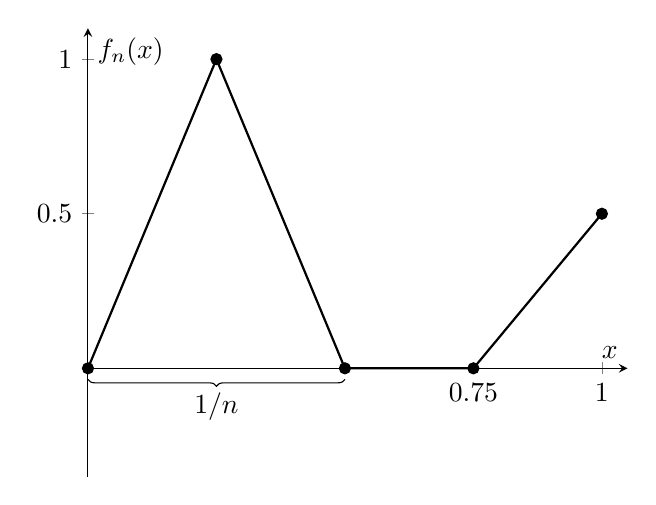
\begin{tikzpicture}
\begin{axis}[
    axis lines = middle,
    xmin = 0, xmax = 1.05,
    ymin = -0.35, ymax = 1.1,
    xlabel = $x$,
    ylabel = {$f_n(x)$},
    xtick = {0.75, 1},
    xticklabels = {$0.75$, $1$},
]

% Piecewise linear function
\addplot[thick] coordinates {
    (0, 0)
    ({1/(2*2)}, 1)
    ({1/2}, 0)
    (0.75, 0)
    (1, 0.5)
};

% Mark key points (optional)
\addplot[only marks, mark=*] coordinates {
    (0, 0)
    ({1/(2*2)}, 1)
    ({1/2}, 0)
    (0.75, 0)
    (1, 0.5)
};

% Bracket under x-axis for [0, 1/n] with label "1/n"
\draw [decorate, decoration={brace, mirror, raise=4pt}]
  (axis cs:0,0) -- (axis cs:{1/2},0)
  node[midway, yshift=-14pt] {$1/n$};

\end{axis}
\end{tikzpicture}

and the function

\begin{tikzpicture}
\begin{axis}[
    axis lines = middle,
    xmin = 0, xmax = 1.05,
    ymin = -0.35, ymax = 1.1,
    xlabel = $x$,
    ylabel = {$f(x)$},
    xtick = {0.75, 1},
    xticklabels = {$0.75$, $1$},
]

% Piecewise linear function
\addplot[thick] coordinates {
    (0, 0)
    (0.75, 0)
    (1, 0.5)
};

% Mark key points (optional)
\addplot[only marks, mark=*] coordinates {
    (0, 0)
    (0.75, 0)
    (1, 0.5)
};
\end{axis}
\end{tikzpicture}

defined on $(0,1)$
We see that
$$
f_n \rightarrow f
$$
pointwise but
$$
\operatorname{argmax}f_n\rightarrow 0, \operatorname{argmax}f=1,
$$
\end{exmp}

\begin{theo}[Consistency of the MLE (Wald)]
Let \(X_1, \dots, X_n \overset{\mathrm{i.i.d.}}{\sim} P_{\theta_0}\), where \(\theta_0 \in \Theta \subset \mathbb{R}^p\).
Assume:

\begin{enumerate}
  \item (Identifiability) \(P_\theta = P_{\theta_0}\) a.s. implies \(\theta = \theta_0\).
  \item (Common domination) \(\{P_\theta : \theta \in \Theta\}\) is dominated by a common $\sigma$-finite measure $\mu$, with density \(f(x \mid \theta)\).
  \item (Compactness) \(\Theta\) is compact.
  \item (Continuity) \(\ell(x, \theta) := \log f(x \mid \theta)\) is continuous in \(\theta\) for $\mu$-a.e.\ $x$.
  \item (Integrability) \(\mathbb{E}_{\theta_0}\!\left[ \sup_{\theta \in \Theta} |\ell(X_1, \theta)| \right] < \infty\).
\end{enumerate}
Then any maximum likelihood estimator
\[
\hat{\theta}_n
\in \arg\max_{\theta \in \Theta} \frac{1}{n} \sum_{i=1}^n \ell(X_i, \theta)
\]
is strongly consistent:
\[
\hat{\theta}_n \xrightarrow{\text{a.s.}} \theta_0.
\]
\end{theo}

\begin{proof}
Define the empirical criterion function
\[
\Delta_n(\theta)
:= \frac{1}{n} \sum_{i=1}^n \ell(X_i, \theta),
\qquad
\Delta(\theta)
:= \mathbb{E}_{\theta_0}[\ell(X_1, \theta)].
\]

\emph{Step 1 (Uniform LLN).}
By the integrability and continuity assumptions and compactness of \(\Theta\),
the class \(\{ \ell(\cdot, \theta) : \theta \in \Theta \}\) is Glivenko--Cantelli.
Hence,
\[
\sup_{\theta \in \Theta} \big| \Delta_n(\theta) - \Delta(\theta) \big|
\xrightarrow{\text{a.s.}} 0.
\]

\emph{Step 2 (Population objective is uniquely maximized at \(\theta_0\)).}
Note that
\[
\Delta(\theta) - \Delta(\theta_0)
= \mathbb{E}_{\theta_0} \!\left[ \log \frac{f(X_1 \mid \theta)}{f(X_1 \mid \theta_0)} \right]
= - \mathrm{KL}\!\left( P_{\theta_0} \,\|\, P_\theta \right) \leq \log\mathbb{E}_{\theta_0} \!\left[ \frac{f(X_1 \mid \theta)}{f(X_1 \mid \theta_0)} \right]
\]
then we have
\[
\mathbb{E}_{\theta_0} \!\left[ \frac{f(X_1 \mid \theta)}{f(X_1 \mid \theta_0)} \right] = \int \frac{f(X_1 \mid \theta)}{f(X_1 \mid \theta_0)}f(X_1 \mid \theta_0)d\mu = \int f(X_1 \mid \theta)d\mu=1
\]
with $\log(1)=0$ we have
\[
\Delta(\theta) - \Delta(\theta_0) \leq 0
\]
with equality if and only if \(P_\theta = P_{\theta_0}\) by the property of Jensen, which by identifiability
implies \(\theta = \theta_0\).
Thus, \(\Delta(\theta)\) is uniquely maximized at \(\theta_0\).

\emph{Step 3 (Argmax continuity).}
By Step 1, \(M_n\) converges uniformly to \(M\), and by Step 2,
\(M\) has a unique maximizer \(\theta_0\) over compact \(\Theta\).
By the argmax continuous mapping theorem,
\[
\hat{\theta}_n \xrightarrow{\text{a.s.}} \theta_0.
\]
\end{proof}
\begin{theo}[Uniform Law of Large Numbers]
Let $\{X_i\}_{i=1}^n$ be i.i.d.\ random variables with common distribution $P$.
Let $\Theta \subset \mathbb{R}^d$ be a parameter space and let 
$m(x,\theta)$ be a measurable real-valued function defined on 
$\mathcal{X} \times \Theta$.

We say that the class $\{m(\cdot,\theta) : \theta \in \Theta\}$ 
satisfies a \emph{Uniform Law of Large Numbers} if
\[
\sup_{\theta \in \Theta}
\left|
\frac{1}{n}\sum_{i=1}^n m(X_i,\theta)
-
\mathbb{E}\big[m(X_1,\theta)\big]
\right|
\xrightarrow{P} 0.
\]
\end{theo}
\begin{theo}[ULLN for MLE]
Let $X_1,\dots,X_n$ be i.i.d.\ with density $f(x;\theta)$.
Define the empirical log-likelihood
\[
\ell_n(\theta)
=
\frac{1}{n}\sum_{i=1}^n \log f(X_i;\theta),
\]
and the population log-likelihood
\[
\ell(\theta)
=
\mathbb{E}\big[\log f(X_1;\theta)\big].
\]
We say that a Uniform Law of Large Numbers holds if
\[
\sup_{\theta \in \Theta}
\left|
\ell_n(\theta) - \ell(\theta)
\right|
\xrightarrow{P} 0.
\]
that is, let
\[
u_i(\theta) = \log(\frac{p_{\theta}(x_i)}{p_{\theta_0}(x_i)})
\]
we have
\[
\sup_{\theta}|\frac{1}{n}\sum u_i^c(\theta)|\rightarrow 0
\]
for $\theta$ in a neighborhood of $\theta_0$
\end{theo}

\begin{theo}[Sufficient condition for ULLN for MLE]
Let $X_1, \dots, X_n$ be i.i.d.\ with density $p_{\theta_0}$.
Let $\Theta \subset \mathbb{R}^d$ be compact.
Define
\[
\ell_n(\theta)
=
\frac{1}{n}\sum_{i=1}^n \log p_\theta(X_i),
\qquad
\ell(\theta)
=
\mathbb{E}_{\theta_0}\!\left[\log p_\theta(X_1)\right].
\]
Assume:
\begin{enumerate}
\item[(1)] (Continuity) For almost every $x$, the map 
$\theta \mapsto \log p_\theta(x)$ is continuous on $\Theta$.
\item[(2)] (Dominating envelope) There exists a measurable function 
$M(x)$ such that
\[
\sup_{\theta \in \Theta}
\left| \log p_\theta(x) \right|
\le M(x),
\]
and
\[
\mathbb{E}_{\theta_0}[M(X_1)] < \infty.
\]
\item[(3)] (Compact parameter space) $\Theta$ is compact.
\end{enumerate}
Then
\[
\sup_{\theta \in \Theta}
\left|
\ell_n(\theta) - \ell(\theta)
\right|
\xrightarrow{P} 0.
\]
That is, the Uniform Law of Large Numbers holds.
\end{theo}
\begin{note}
\[
V_\rho(x)
:=
\sup_{|\theta-\theta_0|<\rho}
\left|
\log p_\theta(x)
\right|,
\qquad
\mathbb{E}_{\theta_0}[V_\rho(X_1)] < \infty,
\]
and
\[
\mathbb{E}_{\theta_0}
\left[
\sup_{|\theta-\theta_0|<\rho}
\left|
\log p_\theta(X_1)
-
\log p_{\theta_0}(X_1)
\right|
\right]
\to 0.
\]
\end{note}

\begin{theo}[Consistency and Score Equation for MLE]
Let $X_1,\dots,X_n$ be i.i.d.\ with density $p_\theta$,
$\theta \in \Theta \subset \mathbb{R}$.
Assume:

\begin{enumerate}
\item[(1)] $\Theta$ is compact
\item[(2)] (Identifiability)
\[
\ell(\theta)
=
\mathbb{E}_{\theta_0}[\log p_\theta(X_1)]
\]
has a unique maximizer at $\theta_0$.
\item[(3)] (Uniform LLN)
\[
\sup_{\theta \in \Theta}
\left|
\ell_n(\theta) - \ell(\theta)
\right|
\xrightarrow{P_{\theta_0}} 0,
\]
where
\[
\ell_n(\theta)
=
\frac{1}{n}\sum_{i=1}^n \log p_\theta(X_i).
\]
\item[(4)] (Differentiability)
For almost every $x$, $\theta \mapsto \log p_\theta(x)$
is continuously differentiable in a neighborhood of $\theta_0$,
and differentiation can be interchanged with expectation.
\end{enumerate}

Then:

\begin{enumerate}
\item[(i)] There exists a measurable maximizer
\[
\hat{\theta}_n \in \arg\max_{\theta \in \Theta} \ell_n(\theta)
\]
such that
\[
\hat{\theta}_n \xrightarrow{P_{\theta_0}} \theta_0.
\]

\item[(ii)] If $\hat{\theta}_n$ lies in the interior of $\Theta$,
then it satisfies the score equation
\[
S_n(\hat{\theta}_n)=0,
\]
where
\[
S_n(\theta)
=
\frac{\partial}{\partial\theta} \ell_n(\theta)
=
\frac{1}{n}\sum_{i=1}^n
\frac{\partial}{\partial\theta}
\log p_\theta(X_i).
\]
\end{enumerate}
\end{theo}
\begin{proof}
\textbf{(i) Consistency.}

By compactness of $\Theta$ and continuity of $\ell_n(\theta)$,
a measurable maximizer $\hat\theta_n$ exists.

By the Uniform Law of Large Numbers,
\[
\sup_{\theta\in\Theta}
|\ell_n(\theta)-\ell(\theta)|
\xrightarrow{P}0.
\]
Since $\ell(\theta)$ has a unique maximizer at $\theta_0$,
the argmax continuous mapping theorem implies
\[
\hat\theta_n \xrightarrow{P} \theta_0.
\]

\textbf{(ii) Score equation and Taylor expansion.}

If $\hat\theta_n$ is an interior maximizer and
$\ell_n$ is differentiable,
then the first-order condition gives
\[
S_n(\hat\theta_n)=0.
\]
Now expand the score around $\theta_0$:
\[
0
=
S_n(\hat\theta_n)
=
S_n(\theta_0)
+
(\hat\theta_n-\theta_0)
S_n'(\tilde\theta_n),
\]
for some $\tilde\theta_n$ on the segment line $\hat\theta_n$
and $\theta_0$ by mean value theorem of calculus. Hence
\[
\hat\theta_n-\theta_0
=
-\frac{S_n(\theta_0)}{S_n'(\tilde\theta_n)}.
\]

\textbf{Fisher information limit.}

We have
\[
S_n(\theta_0)
=
\frac{1}{n}\sum_{i=1}^n
\dot\ell_{\theta_0}(X_i),
\]
where
\[
\mathbb{E}_{\theta_0}[\dot\ell_{\theta_0}(X_1)]=0.
\]
By the LLN,
\[
S_n'(\theta)
=
\frac{1}{n}\sum_{i=1}^n
\ddot\ell_\theta(X_i)
\xrightarrow{P}
\mathbb{E}_{\theta_0}[\ddot\ell_{\theta_0}(X_1)].
\]
But by standard regularity,
\[
\mathbb{E}_{\theta_0}[\ddot\ell_{\theta_0}(X_1)]
=
- I(\theta_0),
\]
where
\[
I(\theta_0)
=
\mathbb{E}_{\theta_0}
\left[
\left(
\frac{\partial}{\partial\theta}
\log p_{\theta_0}(X_1)
\right)^2
\right]
\]
is the Fisher information,
and $I(\theta_0)>0$.

Since $\hat\theta_n \to \theta_0$,
also $\tilde\theta_n \to \theta_0$,
so
\[
S_n'(\tilde\theta_n)
\xrightarrow{P}
- I(\theta_0).
\]
as
\[
|S^\prime_n(\tilde\theta_n) - I(\theta_0)|\leq |S^\prime_n(\tilde\theta_n) - I(\tilde\theta_n)| + |I_n(\tilde\theta_n) - I(\theta_0)|
\]
The first terms goes to 0 by uniform law of large numbers and the second term goes to 0 by contiuity of fisher information function, which requires $l$ to be 3 times differentiable.
\bigskip

\textbf{Conclusion.}

Therefore,
\[
\hat\theta_n-\theta_0
=
\frac{S_n(\theta_0)}{I(\theta_0)}
+
o_P(1).
\]

Since $S_n(\theta_0)\xrightarrow{P}0$ by LLN,
we obtain
\[
\hat\theta_n \xrightarrow{P} \theta_0.
\]

\end{proof}
\begin{note}
    This theorem just demonstrated the existence of a such sequence in the stationary points of likelihood function. This is NOT AN ESTIMATOR. The $\hat{\theta}_n$ itself is not well defined.
\end{note}
\begin{note}
    The reason to choose MLE is that
    $$
    \hat{\theta}_{MLE} \sim AN(\theta_0, I^{-1}(\theta_0)/n)
    $$
    It is the most asymptotically efficient one compared with other unbiased estimators with the Cramer-Rao bound.
\end{note}
\begin{note}
    With
    \[
\hat\theta_n-\theta_0
=
-\frac{S_n(\theta_0)}{S_n'(\tilde\theta_n)}.
\]
we have 
\[
\sqrt{n}(\hat\theta_n-\theta_0)
=
\sqrt{n}(-\frac{S_n(\theta_0)}{S_n'(\tilde\theta_n)})
\]
\end{note}
we have 
$$
\sqrt{n} S_n\left(\theta_0\right) \Rightarrow N\left(0, I\left(\theta_0\right)\right)
$$
with CLT for score function and
$$
S_n'(\tilde\theta_n)\xrightarrow{p}I(\theta_0)
$$
by slutsky's lemma we will have 
\[
\sqrt{n}(\hat\theta_n-\theta_0)
\Rightarrow
N\!\left(0, I(\theta_0)^{-1}\right).
\]
\begin{theo}[Asymptotic Expansion of the MLE]
Let $X_1,\dots,X_n$ be i.i.d.\ with density $p_\theta$, $\theta \in \Theta \subset \mathbb{R}$.
Let
\[
\ell_n(\theta) = \sum_{i=1}^n \log p_\theta(X_i)
\]
be the log-likelihood and define the score
\[
S_i(\theta) = \frac{\partial}{\partial \theta}\log p_\theta(X_i),
\qquad
S_n(\theta) = \sum_{i=1}^n S_i(\theta).
\]

Let $\theta_0$ be the true parameter and assume the usual regularity conditions for MLE.
Let
\[
I(\theta_0)
=
E_{\theta_0}\!\left[S_i(\theta_0)^2\right]
=
- E_{\theta_0}\!\left[\frac{\partial^2}{\partial \theta^2}\log p_\theta(X_1)\Big|_{\theta=\theta_0}\right]
\]
be the Fisher information.

If $\hat\theta_n$ is the MLE satisfying $S_n(\hat\theta_n)=0$, then
\[
\hat\theta_n - \theta_0
=
\frac{1}{n I(\theta_0)}
\sum_{i=1}^n S_i(\theta_0)
+
o_p(n^{-1/2}).
\]

Equivalently,
\[
\sqrt n(\hat\theta_n-\theta_0)
=
\frac{1}{I(\theta_0)}
\frac{1}{\sqrt n}\sum_{i=1}^n S_i(\theta_0)
+
o_p(1).
\]
\end{theo}
\begin{defn}[Estimating Equation]
Let $X_1,\dots,X_n$ be i.i.d.\ observations from a distribution with density
$p_\theta(x)$, where $\theta \in \Theta \subset \mathbb{R}^p$.

An \emph{estimating equation} is an equation of the form
\[
\sum_{i=1}^{n} \psi(X_i,\theta)=0,
\]
where
\[
\psi:\mathcal X \times \Theta \to \mathbb R^p
\]
is called the \emph{estimating function}.

An estimator $\hat\theta_n$ is defined as a solution of
\[
\sum_{i=1}^{n} \psi(X_i,\hat\theta_n)=0.
\]
Typically the estimating function satisfies
\[
E_\theta[\psi(X_1,\theta)]=0,
\]
so the equation is unbiased at the true parameter.
\end{defn}

\begin{exmp}[Maximum Likelihood Estimation as an Estimating Equation]
Suppose $X_1,\dots,X_n$ have density $p_\theta(x)$.
The likelihood function is
\[
L_n(\theta)=\prod_{i=1}^{n} p_\theta(X_i),
\]
and the log-likelihood is
\[
\ell_n(\theta)=\sum_{i=1}^{n}\log p_\theta(X_i).
\]
The score function is
\[
U_n(\theta)
=
\frac{\partial}{\partial\theta}\ell_n(\theta)
=
\sum_{i=1}^{n}
\frac{\partial}{\partial\theta}\log p_\theta(X_i).
\]
The maximum likelihood estimator $\hat\theta_n$ satisfies the
\emph{score equation}
\[
U_n(\hat\theta_n)=0,
\]
which can be written as the estimating equation
\[
\sum_{i=1}^{n}\psi(X_i,\theta)=0
\]
with estimating function
\[
\psi(X_i,\theta)
=
\frac{\partial}{\partial\theta}\log p_\theta(X_i).
\]
Thus the MLE is a special case of estimators defined through
estimating equations.
\end{exmp}
\begin{defn}[Newton's Method]
Let $f:\mathbb{R}\to\mathbb{R}$ be a differentiable function. 
To solve the equation
\[
f(\theta)=0,
\]
Newton's method generates a sequence $\{\theta^{(k)}\}$ by the iteration
\[
\theta^{(k+1)}
=
\theta^{(k)}
-
\frac{f\!\left(\theta^{(k)}\right)}{f'\!\left(\theta^{(k)}\right)},
\qquad k=0,1,2,\dots
\]
starting from an initial value $\theta^{(0)}$.
\end{defn}
\begin{defn}[One-step Newton estimator for the MLE (one-dimensional case)]
Let $X_1,\dots,X_n$ be i.i.d.\ with density $p_\theta$, $\theta \in \Theta \subset \mathbb{R}$.
Define the log-likelihood
\[
\ell_n(\theta) = \sum_{i=1}^n \log p_\theta(X_i).
\]
The MLE $\hat{\theta}_n$ satisfies the score equation
\[
\ell_n'(\theta) = 0.
\]
Suppose $\tilde{\theta}_n$ is an initial consistent estimator of $\theta_0$.
Applying one step of Newton's method to solve $\ell_n'(\theta)=0$ gives the
\emph{one-step Newton estimator}
\[
\hat{\theta}_{1,n}
=
\tilde{\theta}_n
-
\frac{\ell_n'(\tilde{\theta}_n)}{\ell_n''(\tilde{\theta}_n)}.
\]
\end{defn}
\begin{theo}[Consistency and Asymptotic Normality of the One-Step Estimator]
Let $X_1,\dots,X_n$ be i.i.d.\ with density $p_\theta$, $\theta\in\Theta\subset\mathbb{R}$,
and let
\[
f_n(\theta)=\ell_n'(\theta)=\sum_{i=1}^n S_i(\theta),
\qquad
S_i(\theta)=\frac{\partial}{\partial\theta}\log p_\theta(X_i).
\]
Let $\hat\theta_{MLE}$ be the MLE satisfying
\[
f_n(\hat\theta_{MLE})=0 .
\]
Let $\hat\theta_c$ be an initial estimator such that
\[
\hat\theta_c \xrightarrow{P} \theta_0 .
\]
Define the one-step estimator
\[
\hat\theta_{1,n}
=
\hat\theta_c
-
\frac{f_n(\hat\theta_c)}{f_n'(\hat\theta_c)} .
\]

Then
\[
\hat\theta_{1,n} \xrightarrow{P} \theta_0
\]
and
\[
\sqrt n(\hat\theta_{1,n}-\theta_0)
\xrightarrow{d}
N\!\left(0,I(\theta_0)^{-1}\right).
\]
\end{theo}

\begin{proof}
First note that
\[
f_n(\hat\theta_{MLE})=0 .
\]
Apply a Taylor expansion of $f_n(\theta)$ around $\hat\theta_c$:
\[
0
=
f_n(\hat\theta_{MLE})
=
f_n(\hat\theta_c)
+
f_n'(\tilde\theta_n)(\hat\theta_{MLE}-\hat\theta_c)
\]
for some $\tilde\theta_n$ between $\hat\theta_c$ and $\hat\theta_{MLE}$.

Thus
\[
\hat\theta_{MLE}
=
\hat\theta_c
-
\frac{f_n(\hat\theta_c)}{f_n'(\tilde\theta_n)} .
\]
Subtract $\hat\theta_{1,n}$:
\[
\hat\theta_{1,n}-\hat\theta_{MLE}
=
f_n(\hat\theta_c)
\left(
\frac{1}{f_n'(\tilde\theta_n)}
-
\frac{1}{f_n'(\hat\theta_c)}
\right).
\]
Since $\hat\theta_c\to\theta_0$ and $\hat\theta_{MLE}\to\theta_0$, we have
$\tilde\theta_n\to\theta_0$. By the law of large numbers,
\[
\frac{1}{n}f_n'(\theta)
\to
- I(\theta_0)
\quad \text{in probability}.
\]
Hence
\[
f_n'(\tilde\theta_n)
=
- nI(\theta_0)+o_p(n),
\qquad
f_n'(\hat\theta_c)
=
- nI(\theta_0)+o_p(n).
\]
Also
\[
f_n(\hat\theta_c)=O_p(\sqrt n).
\]
Therefore
\[
\hat\theta_{1,n}-\hat\theta_{MLE}
=
O_p(\sqrt n)\cdot O_p(n^{-2})
=
o_p(n^{-1/2}).
\]
Thus
\[
\hat\theta_{1,n}
=
\hat\theta_{MLE}
+
o_p(n^{-1/2}).
\]
Since the MLE satisfies
\[
\sqrt n(\hat\theta_{MLE}-\theta_0)
\xrightarrow{d}
N(0,I(\theta_0)^{-1}),
\]
Slutsky's lemma yields
\[
\sqrt n(\hat\theta_{1,n}-\theta_0)
\xrightarrow{d}
N(0,I(\theta_0)^{-1}).
\]
Consistency follows immediately because $\hat\theta_{MLE}\to\theta_0$ and
$\hat\theta_{1,n}-\hat\theta_{MLE}\to 0$ in probability.
\end{proof}

\begin{theo}[Asymptotic normality from a one-dimensional estimating equation]
Let $X_1,\dots,X_n$ be i.i.d.\ from $P_0$. Let $\psi:\mathcal X\times\Theta\to\mathbb R$ be an estimating
function and define
\[
\Psi_n(\theta):=\frac{1}{n}\sum_{i=1}^n \psi(X_i,\theta),
\qquad
\Psi(\theta):=\mathbb E[\psi(X_1,\theta)].
\]
Assume there exists $\theta_0\in\Theta$ such that $\Psi(\theta_0)=0$, and let $\hat\theta_n$ be a (measurable)
solution of the estimating equation
\[
\Psi_n(\hat\theta_n)=0.
\]
Suppose:
\begin{enumerate}
\item $\hat\theta_n \xrightarrow{P} \theta_0$;
\item $\mathbb E[\psi(X_1,\theta_0)^2]<\infty$;
\item $\Psi$ is differentiable at $\theta_0$ with
\[
A:=\Psi'(\theta_0)=\left.\frac{\partial}{\partial\theta}\mathbb E[\psi(X_1,\theta)]\right|_{\theta=\theta_0}\neq 0;
\]
\item (Regularity for linearization) $\Psi_n'(\tilde\theta_n)\xrightarrow{P}A$ for any $\tilde\theta_n$
between $\hat\theta_n$ and $\theta_0$ (e.g.\ if $\partial_\theta\psi(x,\theta)$ exists near $\theta_0$ and
interchange of differentiation and expectation is justified).
\end{enumerate}
Let
\[
B:=\operatorname{Var}\!\big(\psi(X_1,\theta_0)\big).
\]
Then
\[
\sqrt{n}\,(\hat\theta_n-\theta_0)
=
-\frac{1}{A}\,\frac{1}{\sqrt{n}}\sum_{i=1}^n \psi(X_i,\theta_0) + o_p(1),
\]
and hence
\[
\sqrt{n}\,(\hat\theta_n-\theta_0)\;\xrightarrow{d}\;N\!\left(0,\frac{B}{A^2}\right)
\]
\end{theo}
\begin{note}
    Note that
    \[
    \frac{B}{A^2} = V(\theta_0)\geq \frac{1}{I(\theta_0)}
    \]
    which call that MLE is efficient
\end{note}
\begin{note}
    Let
\[
\Psi(\theta) := E_{\theta_0}\!\left[\psi(X_1,\theta)\right].
\]
Assume that
\[
\Psi(\theta_0) = 0
\]
and that $\theta_0$ is the unique solution of the population estimating equation:
\[
E_{\theta_0}\!\left[\psi(X_1,\theta)\right] = 0
\quad \Longleftrightarrow \quad
\theta = \theta_0 .
\]
A standard condition ensuring consistency of an estimator defined by the estimating equation is that the population estimating equation has a unique root at the true parameter.
\end{note}

\begin{exmp}[Estimating equation from the Cox partial likelihood]
Suppose we observe survival data $(T_i,\delta_i,Z_i)$ for $i=1,\dots,n$, where
\begin{itemize}
\item $T_i$ is the observed time,
\item $\delta_i$ is the failure indicator,
\item $Z_i \in \mathbb{R}^p$ is a covariate vector.
\end{itemize}
The Cox proportional hazards model assumes the hazard
\[
\lambda(t|Z_i) = \lambda_0(t)\exp(\beta^\top Z_i),
\]
where $\lambda_0(t)$ is an unspecified baseline hazard and $\beta$ is the parameter of interest.

The Cox \emph{partial likelihood} is
\[
L_p(\beta)
=
\prod_{i:\delta_i=1}
\frac{\exp(\beta^\top Z_i)}
{\sum_{j\in R(T_i)} \exp(\beta^\top Z_j)},
\]
where $R(T_i)$ is the risk set just before time $T_i$.

The log partial likelihood is
\[
\ell_p(\beta)
=
\sum_{i=1}^n
\delta_i
\left[
\beta^\top Z_i
-
\log
\left(
\sum_{j\in R(T_i)} \exp(\beta^\top Z_j)
\right)
\right].
\]
Taking derivative with respect to $\beta$ gives the \emph{score estimating equation}
\[
U_n(\beta)
=
\sum_{i=1}^n
\delta_i
\left(
Z_i -
\frac{\sum_{j\in R(T_i)} Z_j \exp(\beta^\top Z_j)}
{\sum_{j\in R(T_i)} \exp(\beta^\top Z_j)}
\right)
=0 .
\]
The estimator $\hat{\beta}$ is defined as the solution to the estimating equation
\[
U_n(\beta)=0 .
\]
Equivalently, it has the form
\[
\frac{1}{n}\sum_{i=1}^n \psi_i(\beta)=0,
\]
where
\[
\psi_i(\beta)
=
\delta_i
\left(
Z_i -
\frac{\sum_{j\in R(T_i)} Z_j \exp(\beta^\top Z_j)}
{\sum_{j\in R(T_i)} \exp(\beta^\top Z_j)}
\right).
\]
Suppose $(T_i,\delta_i,Z_i), i=1,\dots,n$ are i.i.d. observations from the Cox
proportional hazards model
\[
\lambda(t|Z)=\lambda_0(t)\exp(\beta_0^\top Z).
\]
Let $\hat\beta$ be the estimator obtained by solving the partial likelihood
score equation
\[
U_n(\beta)=\sum_{i=1}^n
\delta_i
\left(
Z_i -
\frac{\sum_{j\in R(T_i)} Z_j \exp(\beta^\top Z_j)}
{\sum_{j\in R(T_i)} \exp(\beta^\top Z_j)}
\right)=0.
\]

Under standard regularity conditions:

\begin{enumerate}
\item \textbf{Consistency}
\[
\hat\beta \xrightarrow{P} \beta_0 .
\]

\item \textbf{Asymptotic normality}
\[
\sqrt{n}(\hat\beta-\beta_0)
\Rightarrow
N\!\left(0, I(\beta_0)^{-1}\right),
\]
where
\[
I(\beta_0)
=
\lim_{n\to\infty}\frac{1}{n}
E\!\left[-\frac{\partial U_n(\beta_0)}{\partial \beta}\right]
\]
is the information matrix associated with the partial likelihood.

\item \textbf{Asymptotic linear representation}
\[
\sqrt{n}(\hat\beta-\beta_0)
=
I(\beta_0)^{-1}
\frac{1}{\sqrt{n}}
\sum_{i=1}^n
\psi_i(\beta_0)
+o_p(1),
\]
where
\[
\psi_i(\beta_0)
=
\delta_i
\left(
Z_i -
\frac{\sum_{j\in R(T_i)} Z_j \exp(\beta_0^\top Z_j)}
{\sum_{j\in R(T_i)} \exp(\beta_0^\top Z_j)}
\right).
\]
\end{enumerate}
\end{exmp}

\begin{exmp}[Estimating equation from a pseudo-likelihood: logistic regression]
Suppose $(Y_i,X_i), i=1,\dots,n$ are i.i.d., where
\[
Y_i \in \{0,1\}, \qquad X_i \in \mathbb{R}^p .
\]
Assume the conditional mean model
\[
P(Y_i=1\mid X_i)=\mu_i(\beta)
=
\frac{\exp(X_i^\top\beta)}{1+\exp(X_i^\top\beta)} .
\]
The Bernoulli likelihood leads to the log pseudo-likelihood
\[
\ell_n(\beta)
=
\sum_{i=1}^n
\left[
Y_i X_i^\top\beta
-
\log(1+\exp(X_i^\top\beta))
\right].
\]
Taking derivative gives the estimating equation
\[
U_n(\beta)
=
\sum_{i=1}^n
X_i\big(Y_i-\mu_i(\beta)\big)
=
0.
\]
Equivalently,
\[
\frac{1}{n}\sum_{i=1}^n \psi_i(\beta)=0,
\qquad
\psi_i(\beta)=X_i\big(Y_i-\mu_i(\beta)\big).
\]
The estimator $\hat\beta$ is defined as the solution to
\[
U_n(\beta)=0 .
\]
Assume regularity conditions:
\begin{enumerate}
\item $E\|X_i\|^2<\infty$,
\item the parameter space is compact and $\beta_0$ is interior,
\item the population estimating equation has a unique root:
\[
E[\psi_i(\beta)]=0 \quad \Longleftrightarrow \quad \beta=\beta_0.
\]
\end{enumerate}
Then the estimator $\hat\beta$ satisfying
\[
\frac{1}{n}\sum_{i=1}^n \psi_i(\beta)=0
\]
has the following properties.

\textbf{(1) Consistency}
\[
\hat\beta \xrightarrow{P} \beta_0 .
\]

\textbf{(2) Asymptotic normality}
\[
\sqrt n(\hat\beta-\beta_0)
\Rightarrow
N\!\left(0, A^{-1} B A^{-1}\right),
\]
where
\[
A
=
E\!\left[
-\frac{\partial \psi_i(\beta_0)}{\partial\beta}
\right],
\qquad
B
=
\operatorname{Var}\!\big(\psi_i(\beta_0)\big).
\]

\textbf{(3) Asymptotic linear representation}
\[
\sqrt n(\hat\beta-\beta_0)
=
A^{-1}
\frac{1}{\sqrt n}
\sum_{i=1}^n
\psi_i(\beta_0)
+
o_p(1).
\]
\end{exmp}
\begin{exmp}[General Method of Moments (MoM) as an estimating equation]
Let $X_1,\dots,X_n$ be i.i.d.\ with distribution $P_{\theta_0}$, where
$\theta_0\in\Theta\subset\mathbb{R}^p$.
Let $m:\mathcal{X}\times\Theta\to\mathbb{R}^p$ be a vector of moment functions such that
\[
E_{\theta_0}\big[m(X_1,\theta_0)\big]=0.
\]
Define the sample moment (estimating) function
\[
g_n(\theta):=\frac{1}{n}\sum_{i=1}^n m(X_i,\theta).
\]

\textbf{(Just-identified MoM, $p$ moments for $p$ parameters).}
The method-of-moments estimator $\hat\theta_n$ is defined as any solution to the estimating equation
\[
g_n(\theta)=0,
\qquad\text{i.e.,}\qquad
\frac{1}{n}\sum_{i=1}^n m(X_i,\theta)=0.
\]
\end{exmp}

\begin{theo}[Asymptotic properties of (just-identified) MoM estimators]
Assume:

\begin{enumerate}
\item[(A1)] (\textbf{Identification}) The population moment equation has a unique solution:
\[
E_{\theta_0}\big[m(X_1,\theta)\big]=0 \quad\Longleftrightarrow\quad \theta=\theta_0.
\]
\item[(A2)] (\textbf{Uniform law of large numbers})
\[
\sup_{\theta\in\Theta}\big\|g_n(\theta)-g(\theta)\big\|\xrightarrow{P}0,
\qquad
g(\theta):=E_{\theta_0}[m(X_1,\theta)].
\]
\item[(A3)] (\textbf{Smoothness}) $g(\theta)$ is continuously differentiable in a neighborhood of $\theta_0$ and
\[
A:=\nabla_\theta g(\theta_0) \in \mathbb{R}^{p\times p}
\quad\text{is nonsingular.}
\]
\item[(A4)] (\textbf{CLT for moments}) $E_{\theta_0}\|m(X_1,\theta_0)\|^2<\infty$, so that
\[
\frac{1}{\sqrt{n}}\sum_{i=1}^n m(X_i,\theta_0)\Rightarrow N(0,B),
\qquad
B:=\operatorname{Var}_{\theta_0}\!\big(m(X_1,\theta_0)\big).
\]
\end{enumerate}

Let $\hat\theta_n$ satisfy $g_n(\hat\theta_n)=0$. Then:

\textbf{(1) Consistency}
\[
\hat\theta_n\xrightarrow{P}\theta_0.
\]

\textbf{(2) Asymptotic linearity}
\[
\sqrt{n}(\hat\theta_n-\theta_0)
=
-\,A^{-1}\frac{1}{\sqrt{n}}\sum_{i=1}^n m(X_i,\theta_0)
+o_p(1).
\]

\textbf{(3) Asymptotic normality}
\[
\sqrt{n}(\hat\theta_n-\theta_0)\Rightarrow N\!\big(0,\ A^{-1}BA^{-T}\big).
\]
\end{theo}
\begin{exmp}[Mis-specified model MLE (Quasi-MLE) as an estimating equation; sandwich asymptotics]
Let $X_1,\dots,X_n$ be i.i.d.\ from an unknown true distribution $P_0$.
We nevertheless fit a parametric family $\{p_\theta:\theta\in\Theta\subset\mathbb R^d\}$,
which may be mis-specified (i.e.\ $P_0\notin\{P_\theta\}$).

Define the (quasi-)log-likelihood
\[
\ell_n(\theta)=\sum_{i=1}^n \log p_\theta(X_i),
\qquad
\hat\theta_n \in \arg\max_{\theta\in\Theta}\ell_n(\theta).
\]
Let the score (estimating function) be
\[
\psi(x,\theta):=\nabla_\theta \log p_\theta(x),
\qquad
\Psi_n(\theta):=\frac1n\sum_{i=1}^n \psi(X_i,\theta).
\]
Then any interior maximizer $\hat\theta_n$ satisfies the estimating equation
\[
\Psi_n(\hat\theta_n)=0.
\]
\noindent\textbf{Pseudo-true parameter.}
Define the population objective
\[
Q(\theta):=\mathbb E_0\big[\log p_\theta(X_1)\big],
\]
and assume $Q$ has a unique maximizer $\theta^\star$ in the interior of $\Theta$.
Under differentiability and interchange of derivative and expectation,
$\theta^\star$ also solves the population estimating equation
\[
\Psi(\theta):=\mathbb E_0[\psi(X_1,\theta)]=0
\quad\text{at}\quad \theta=\theta^\star.
\]
(Equivalently, $\theta^\star$ is the KL projection of $P_0$ onto the model.)

\noindent\textbf{Asymptotic normality (sandwich form).}
Assume $\psi(x,\theta)$ is continuously differentiable in a neighborhood of $\theta^\star$,
$\mathbb E_0\|\psi(X_1,\theta^\star)\|^2<\infty$, and the matrix
\[
A:=-\mathbb E_0\!\left[\nabla_\theta \psi(X_1,\theta^\star)\right]
\]
is nonsingular. Let
\[
B:=\mathbb E_0\!\left[\psi(X_1,\theta^\star)\psi(X_1,\theta^\star)^\top\right].
\]
Then
\[
\sqrt{n}\,(\hat\theta_n-\theta^\star)
\ \Rightarrow\
N\!\left(0,\ A^{-1}BA^{-1\top}\right).
\]
Moreover, the asymptotic linear expansion holds:
\[
\hat\theta_n-\theta^\star
=
\frac1n\sum_{i=1}^n A^{-1}\psi(X_i,\theta^\star)
+o_p(n^{-1/2}).
\]
\noindent\textbf{Remark.}
If the model is correctly specified, i.e.\ $P_0=P_{\theta_0}$ for some $\theta_0$,
then $\theta^\star=\theta_0$ and typically $B=A$ (information identity),
so the covariance reduces to $A^{-1}$ (the usual MLE Fisher-information form).
Under mis-specification, generally $B\neq A$, yielding the robust ``sandwich'' variance.
\end{exmp}
\begin{lemma}[Lindeberg Central Limit Theorem]
Let $X_1,\dots,X_n$ be independent random variables with densities
\[
f(x_i,\theta,z_i),
\]
where $\theta$ is a parameter and $z_i$ are known covariates (design points).  
Define
\[
\mu_i(\theta)=\mathbb{E}_\theta[X_i], \qquad 
\sigma_i^2(\theta)=\mathrm{Var}_\theta(X_i),
\]
and let
\[
s_n^2(\theta)=\sum_{i=1}^n \sigma_i^2(\theta).
\]

Assume $s_n^2(\theta)\to\infty$ as $n\to\infty$. Suppose the following
\emph{Lindeberg condition} holds: for every $\varepsilon>0$,
\[
\frac{1}{s_n^2(\theta)}
\sum_{i=1}^n
\mathbb{E}_\theta\!\left[
(X_i-\mu_i(\theta))^2
\mathbf{1}\!\left(
|X_i-\mu_i(\theta)|>\varepsilon s_n(\theta)
\right)
\right]
\longrightarrow 0.
\]

Then
\[
\frac{\sum_{i=1}^n (X_i-\mu_i(\theta))}{s_n(\theta)}
\;\xrightarrow{d}\;
N(0,1).
\]
\end{lemma}
\begin{defn}[Cesàro Sum]
Let $\{a_n\}_{n\ge1}$ be a sequence and let
\[
s_n=\sum_{k=1}^n a_k
\]
be the sequence of partial sums.
The \emph{Cesàro means} of the sequence $\{s_n\}$ are defined by
\[
\sigma_n
=
\frac{1}{n}\sum_{k=1}^n s_k .
\]

If $\sigma_n \to s$ as $n\to\infty$, then the series
\[
\sum_{n=1}^{\infty} a_n
\]
is said to be \emph{Cesàro summable} (or has \emph{Cesàro sum}) $s$.
\end{defn}
\begin{lemma}[Lindeberg Central Limit Theorem (Cesàro Form)]
Let $Y_{n1},\dots,Y_{nn}$ be independent random vectors in $\mathbb{R}^p$
such that
\[
\mathbb{E}[Y_{ni}] = 0 .
\]

Define
\[
S_n = \sum_{i=1}^n Y_{ni}.
\]

Assume the Cesàro variance limit exists:
\[
\frac{1}{n}\mathrm{Var}(S_n)
=
\frac{1}{n}\sum_{i=1}^n \mathrm{Var}(Y_{ni})
\;\longrightarrow\;
M ,
\]
where $M$ is a finite positive semidefinite matrix.

Assume the Lindeberg condition holds: for every $\varepsilon>0$,
\[
\frac{1}{n}
\sum_{i=1}^n
\mathbb{E}\!\left[
\|Y_{ni}\|^2
\mathbf{1}\!\left(
\|Y_{ni}\|>\varepsilon\sqrt{n}
\right)
\right]
\longrightarrow 0 .
\]

Then
\[
\frac{1}{\sqrt{n}}S_n
=
\frac{1}{\sqrt{n}}\sum_{i=1}^n Y_{ni}
\;\xrightarrow{d}\;
N(0,M).
\]
\end{lemma}
\begin{lemma}[Law of Large Numbers for Independent Non-Identically Distributed Observations]
Let $X_1,X_2,\dots,X_n$ be independent random variables with densities
\[
f(x_i,\theta,z_i),
\]
where $\theta$ is a parameter and $z_i$ are known covariates. Assume that each $X_i$ has a finite mean
\[
\mu_i(\theta)=\mathbb{E}_\theta[X_i].
\]

If
\[
\frac{1}{n^2}\sum_{i=1}^n \mathrm{Var}_\theta(X_i) \;\longrightarrow\; 0,
\]
then
\[
\frac{1}{n}\sum_{i=1}^n \left(X_i-\mu_i(\theta)\right)
\;\xrightarrow{p}\; 0,
\]
that is,
\[
\frac{1}{n}\sum_{i=1}^n X_i
-
\frac{1}{n}\sum_{i=1}^n \mu_i(\theta)
\;\xrightarrow{p}\; 0 .
\]
\end{lemma}
\begin{theo}[Asymptotic Normality of the MLE: Multivariate Non-i.i.d. Case]
Let $X_1,\dots,X_n$ be independent observations with densities
\[
f(x_i,\theta,z_i)
\]
with respect to a dominating measure $\mu$, where $\theta\in\Theta\subset\mathbb{R}^p$
is the parameter vector and $z_i$ are known covariates. Let the log-likelihood be
\[
\ell_n(\theta)=\sum_{i=1}^n \log f(X_i,\theta,z_i).
\]
Define the score vector
\[
S_n(\theta)
=
\frac{\partial}{\partial\theta}\ell_n(\theta)
=
\sum_{i=1}^n s_i(\theta),
\qquad
s_i(\theta)=\frac{\partial}{\partial\theta}\log f(X_i,\theta,z_i),
\]
and the Hessian matrix
\[
S_n'(\theta)
=
\frac{\partial}{\partial\theta^\top}S_n(\theta)
=
\frac{\partial^2}{\partial\theta\partial\theta^\top}\ell_n(\theta).
\]
Let $\hat\theta_n$ denote the maximum likelihood estimator and let the
true parameter be $\theta_0$.

Assume:
\begin{enumerate}
\item $\theta_0$ lies in the interior of $\Theta$, and differentiation
under the integral sign is valid since $f(x,\theta,z)$ is dominated by $\mu$.
\item The score has mean zero
\[
\mathbb{E}_{\theta_0}[s_i(\theta_0)]=0 .
\]
\item The Lindeberg condition holds for the triangular array
$\{s_i(\theta_0)\}$, so that
\[
\frac{1}{\sqrt{n}}S_n(\theta_0)
=
\frac{1}{\sqrt{n}}\sum_{i=1}^n s_i(\theta_0)
\xrightarrow{d}
N(0,M),
\]
where
\[
M
=
\lim_{n\to\infty}
\frac{1}{n}\mathrm{Var}\big(S_n(\theta_0)\big).
\]
\item The observed information satisfies a law of large numbers
\[
-\frac{1}{n}S_n'(\theta_0)
=
-\frac{1}{n}\sum_{i=1}^n
\frac{\partial^2}{\partial\theta\partial\theta^\top}
\log f(X_i,\theta_0,z_i)
\xrightarrow{p}
B,
\]
where
\[
B
=
\lim_{n\to\infty}
\frac{1}{n}\sum_{i=1}^n
\mathbb{E}_{\theta_0}
\!\left[
-
\frac{\partial^2}{\partial\theta\partial\theta^\top}
\log f(X_i,\theta_0,z_i)
\right].
\]
\end{enumerate}
Then
\[
\sqrt{n}(\hat\theta_n-\theta_0)
\xrightarrow{d}
N\!\left(0,\,B^{-1}MB^{-1}\right).
\]
If the model is correctly specified so that the information equality holds
($M=B$), then
\[
\sqrt{n}(\hat\theta_n-\theta_0)
\xrightarrow{d}
N(0,B^{-1}).
\]
\end{theo}
\begin{defn}[Estimation of $B$ and $M$]
Let $\hat\theta_n$ be the MLE. Define the empirical estimators of $B$ and $M$ by
plugging in $\hat\theta_n$.

The estimator of $B$ (the limit of the observed information) is
\[
\hat B_n
=
-\frac{1}{n}S_n'(\hat\theta_n)
=
-\frac{1}{n}\sum_{i=1}^n
\frac{\partial^2}{\partial\theta\partial\theta^\top}
\log f(X_i,\hat\theta_n,z_i).
\]

The estimator of $M$ (the variance of the score) is
\[
\hat M_n
=
\frac{1}{n}\sum_{i=1}^n
s_i(\hat\theta_n)s_i(\hat\theta_n)^\top,
\]
where
\[
s_i(\hat\theta_n)
=
\frac{\partial}{\partial\theta}
\log f(X_i,\hat\theta_n,z_i).
\]
Note that here Var is a deterministic simple function, it may have variations.
\end{defn}
\begin{defn}[Estimated Asymptotic Covariance of the MLE]
The asymptotic covariance matrix of $\hat\theta_n$ can be estimated by the
sandwich estimator
\[
\widehat{\mathrm{Var}}(\hat\theta_n)
=
\frac{1}{n}
\hat B_n^{-1}\hat M_n\hat B_n^{-1}.
\]
\end{defn}
If the model is correctly specified so that the information equality holds,
then $\hat M_n=\hat B_n$ asymptotically and the covariance estimator reduces to
\[
\widehat{\mathrm{Var}}(\hat\theta_n)
=
\frac{1}{n}\hat B_n^{-1}.
\]
\begin{defn}[Asymptotic Test for a Single Parameter]
Consider testing
\[
H_0:\theta_j=\theta_{j0}.
\]
The test statistic is
\[
Z_j
=
\frac{\hat\theta_j-\theta_{j0}}
{\sqrt{\hat\Sigma_{jj}/n}}.
\]
with $\Sigma = B^{-1}MB^{-1}$ and $\hat\Sigma=
\hat B_n^{-1}\hat M_n\hat B_n^{-1}.$
Then
\[
Z_j \xrightarrow{d} N(0,1).
\]
Reject $H_0$ at level $\alpha$ if
\[
|Z_j|>z_{\alpha/2}.
\]
Equivalently,
\[
Z_j^2 \xrightarrow{d} \chi^2_1.
\]
\end{defn}
\begin{defn}[Joint Wald Test for the Parameter Vector]
To test
\[
H_0:\theta=\theta_0,
\]
the Wald statistic is
\[
W
=
n(\hat\theta-\theta_0)^\top
\hat\Sigma^{-1}
(\hat\theta-\theta_0).
\]
Then
\[
W \xrightarrow{d} \chi^2_p,
\]
where $p$ is the dimension of $\theta$.
Reject $H_0$ if
\[
W>\chi^2_{p,\alpha}.
\]
\end{defn}
\newpage
\section{U-statistics}
\begin{defn}
A \emph{U-statistic} based on i.i.d.\ observations \(X_1,\dots,X_n\) is a statistic of the form
\[
U_n=\binom{n}{m}^{-1}\sum_{1\le i_1<\cdots<i_m\le n} h(X_{i_1},\dots,X_{i_m}),
\]
where \(m\) is a fixed positive integer and \(h\) is a symmetric measurable function of \(m\) variables, called the kernel. Symmetric means that for any permutation \(\pi\),
\[
h(x_1,\dots,x_m)=h(x_{\pi(1)},\dots,x_{\pi(m)}).
\]
The U-statistic \(U_n\) is an unbiased estimator of
\[
\theta = E\bigl[h(X_1,\dots,X_m)\bigr].
\]
\end{defn}

\begin{defn}
A \emph{V-statistic} based on i.i.d.\ observations \(X_1,\dots,X_n\) is a statistic of the form
\[
V_n=\frac{1}{n^m}\sum_{i_1=1}^n \cdots \sum_{i_m=1}^n h(X_{i_1},\dots,X_{i_m}),
\]
where \(m\) is a fixed positive integer and \(h\) is a measurable function of \(m\) variables, called the kernel. If \(h\) is symmetric, then \(V_n\) is called a symmetric V-statistic.
\end{defn}
\begin{exmp}
    For \(m=1\), let
\[
h(X_i)=X_i.
\]
Then the corresponding U-statistic is
\[
U_n=\binom{n}{1}^{-1}\sum_{i=1}^n h(X_i)
=\frac{1}{n}\sum_{i=1}^n X_i
=\bar X,
\]
which is an unbiased estimator of
\[
\mu=E(X_i).
\]
\end{exmp}
\begin{exmp}
    For \(m=2\), take the symmetric kernel
\[
h(X_i,X_j)=X_iX_j.
\]
Then the corresponding U-statistic is
\[
U_n=\binom{n}{2}^{-1}\sum_{1\le i<j\le n} X_iX_j.
\]
Since \(X_i\) and \(X_j\) are i.i.d. for \(i\ne j\),
\[
E\bigl[h(X_i,X_j)\bigr]=E(X_iX_j)=E(X_i)E(X_j)=\mu^2.
\]
Hence
\[
U_n=\binom{n}{2}^{-1}\sum_{1\le i<j\le n} X_iX_j = (\frac{n}{n-1})(\bar{X}^2-\frac{\sum_{i=1}^n X_i^2}{n(n-1)})
\]
is a U-statistic of degree \(2\) that is an unbiased estimator of \(\mu^2\).
\end{exmp}
\begin{note}
    Let $\hat\theta = \bar{X}^2$, we have bias $B(\hat\theta) = O(1/n)$ and variance $V(\hat\theta) = O(1/n)$ 
\end{note}
\begin{exmp}
    For \(m=2\), take the symmetric kernel
\[
h(X_i,X_j)=\frac{(X_i-X_j)^2}{2}.
\]
Then the corresponding U-statistic is
\[
U_n=\binom{n}{2}^{-1}\sum_{1\le i<j\le n}\frac{(X_i-X_j)^2}{2}.
\]
Since \(X_i\) and \(X_j\) are i.i.d.,
\[
E\left[\frac{(X_i-X_j)^2}{2}\right]
=\frac{1}{2}E\left(X_i^2-2X_iX_j+X_j^2\right)
=\frac{1}{2}\bigl(E(X_i^2)-2E(X_i)E(X_j)+E(X_j^2)\bigr)
=\sigma^2.
\]
Hence
\[
U_n=\binom{n}{2}^{-1}\sum_{1\le i<j\le n}\frac{(X_i-X_j)^2}{2}
\]
is a U-statistic of degree \(2\) that is an unbiased estimator of \(\sigma^2\).
\end{exmp}
\begin{note}
    Since
\[
(X_i-X_j)^2=X_i^2-2X_iX_j+X_j^2,
\]
we have
\[
\frac{(X_i-X_j)^2}{2}
=\frac{X_i^2+X_j^2}{2}-X_iX_j.
\]

Therefore the kernel
\[
h(X_i,X_j)=\frac{(X_i-X_j)^2}{2}
\]
can be written equivalently as
\[
h(X_i,X_j)=\frac{X_i^2+X_j^2}{2}-X_iX_j.
\]

Because the kernel is symmetric in \(i\) and \(j\), this is often informally written as
\[
h(X_i,X_j)=X_i^2-X_iX_j,
\]
meaning that after averaging over all unordered pairs \((i,j)\), the two forms are the same.

Indeed,
\[
\binom{n}{2}^{-1}\sum_{1\le i<j\le n}\frac{X_i^2+X_j^2}{2}
=
\binom{n}{2}^{-1}\sum_{1\le i<j\le n} X_i^2,
\]
by symmetry, so
\[
\binom{n}{2}^{-1}\sum_{1\le i<j\le n}\frac{(X_i-X_j)^2}{2}
=
\binom{n}{2}^{-1}\sum_{1\le i<j\le n}(X_i^2-X_iX_j).
\]

Hence the U-statistic may also be written as
\[
U_n
=
\binom{n}{2}^{-1}\sum_{1\le i<j\le n}(X_i^2-X_iX_j).
\]
\end{note}
\begin{exmp}
    Suppose \(X_1,\dots,X_n\) are i.i.d., and we want to test symmetry about \(1/2\).  
Then a degree-\(2\) U-statistic can be constructed from the symmetric kernel
\[
h(X_i,X_j)=\mathbf 1\{X_i+X_j>1\}.
\]
The corresponding U-statistic is
\[
U_n=\binom{n}{2}^{-1}\sum_{1\le i<j\le n}\mathbf 1\{X_i+X_j>1\}.
\]

Under the null hypothesis that the distribution is symmetric about \(1/2\),
\[
X-\tfrac12 \overset{d}= -(X-\tfrac12),
\]
which implies
\[
P(X_i+X_j>1)=\frac12
\]
(for continuous distributions, so that \(P(X_i+X_j=1)=0\)). Hence
\[
E(U_n)=\frac12
\]
under \(H_0\).
Therefore,
\[
U_n=\binom{n}{2}^{-1}\sum_{1\le i<j\le n}\mathbf 1\{X_i+X_j>1\}
\]
is a degree-\(2\) U-statistic that can be used to test symmetry about \(1/2\), with null value \(1/2\).
\end{exmp}
\begin{note}
    This does not only test 0 median, it tests symmetry, which is a stronger condition for 0 median
\end{note}
\begin{theo}
Let
\[
E\bigl[h(X_1,\dots,X_m)^2\bigr]<\infty.
\]
Then
\[
E\bigl(U_n-V_n\bigr)^2=O\!\left(n^{-2}\right).
\]
Hence,
\[
U_n-V_n=O_p(n^{-1}).
\]
\end{theo}
\begin{theo}
Let \(U_n\) be a U-statistic and \(V_n\) the corresponding V-statistic based on a symmetric kernel \(h\) of degree \(m\). Assume
\[
E\bigl[h(X_1,\dots,X_m)^2\bigr]<\infty,
\]
and suppose that for some parameter \(\theta\),
\[
U_n-\theta=\frac1n\sum_{i=1}^n A^c(\theta,X_i)+o_p(n^{-1/2}),
\]
Then \(V_n\) has the same asymptotic linear representation:
\[
V_n-\theta=\frac1n\sum_{i=1}^n A^c(\theta,X_i)+o_p(n^{-1/2}).
\]
Consequently,
\[
\sqrt n\,(V_n-\theta)\xrightarrow{d}N\!\left(0,\operatorname{Var}\!\bigl(A^c(\theta,X_1)\bigr)\right),
\]
so \(U_n\) and \(V_n\) have the same asymptotic normality and the same influence function \(A^c(\theta,X_i)\).
\end{theo}
\begin{proof}
From the previous result,
\[
E(U_n-V_n)^2=O(n^{-2}),
\]
hence
\[
U_n-V_n=O_p(n^{-1}).
\]
Therefore
\[
\sqrt n\,(U_n-V_n)=O_p(n^{-1/2})=o_p(1).
\]

Now write
\[
V_n-\theta
=
(U_n-\theta)-(U_n-V_n).
\]
Using the assumed asymptotic linear representation of \(U_n\),
\[
V_n-\theta
=
\left\{\frac1n\sum_{i=1}^n A^c(\theta,X_i)+o_p(n^{-1/2})\right\}
-
(U_n-V_n).
\]
Since \(U_n-V_n=O_p(n^{-1})=o_p(n^{-1/2})\), it follows that
\[
V_n-\theta
=
\frac1n\sum_{i=1}^n A^c(\theta,X_i)+o_p(n^{-1/2}).
\]
Thus \(V_n\) has the same influence function \(A^c(\theta,X_i)\).

Multiplying by \(\sqrt n\),
\[
\sqrt n\,(V_n-\theta)
=
\frac1{\sqrt n}\sum_{i=1}^n A^c(\theta,X_i)+o_p(1).
\]
Because \(E[A^c(\theta,X_i)]=0\), the central limit theorem gives
\[
\frac1{\sqrt n}\sum_{i=1}^n A^c(\theta,X_i)
\xrightarrow{d}
N\!\left(0,\operatorname{Var}(A^c(\theta,X_1))\right).
\]
Hence, by Slutsky's theorem,
\[
\sqrt n\,(V_n-\theta)\xrightarrow{d}N\!\left(0,\operatorname{Var}(A^c(\theta,X_1))\right).
\]

Since the same limit holds for \(U_n\), the U-statistic and the corresponding V-statistic have the same asymptotic normal distribution and the same influence function.
\end{proof}

\begin{defn}[First-order projection function]
Let $h(x_1,\dots,x_m)$ be a symmetric kernel with
\[
\theta = \mathbb{E}[h(X_1,\dots,X_m)].
\]
The first-order projection function $h_1(x)$ is defined as
\[
h_1(x)
=
\mathbb{E}[\,h(X_1, X_2,\dots,X_m)\,\mid X_1 = x] - \theta,
\]
where $X_2,\dots,X_m \overset{i.i.d.}{\sim} F$ are independent of $x$. Also we denote
\[
h_1^c(X_i)
=
\mathbb{E}[\,h(X_1, X_2,\dots,X_m)\,\mid X_i = x] - \theta,
\]
\end{defn}

\begin{theo}[Hájek projection for U-statistics]
Let
\[
U_n
=
\binom{n}{m}^{-1}
\sum_{1 \le i_1 < \cdots < i_m \le n}
h(X_{i_1},\dots,X_{i_m}),
\]
where $h$ is a symmetric kernel of degree $m$, and let
\[
\theta = \mathbb{E}[h(X_1,\dots,X_m)].
\]
Define the centered kernel
\[
h^c(x_1,\dots,x_m) := h(x_1,\dots,x_m)-\theta,
\]
and define
\[
h_1(x):=\mathbb{E}[h(x,X_2,\dots,X_m)],
\qquad
h_1^c(x):=h_1(x)-\theta
=\mathbb{E}[h^c(x,X_2,\dots,X_m)].
\]
Then the first-order (Hájek) projection of $U_n$ is
\[
U_n^{(1)}
=
\theta+\frac{m}{n}\sum_{i=1}^n h_1^c(X_i).
\]
Equivalently,
\[
U_n^{(1)}-\theta
=
\frac{m}{n}\sum_{i=1}^n h_1^c(X_i).
\]
\end{theo}

\begin{proof}
By the general definition of the first-order projection,
\[
U_n^{(1)}
=
\mathbb{E}[U_n]
+
\sum_{i=1}^n\Bigl(\mathbb{E}[U_n\mid X_i]-\mathbb{E}[U_n]\Bigr).
\]
Since $U_n$ is a U-statistic with kernel mean $\theta$,
\[
\mathbb{E}[U_n]=\theta.
\]
Hence it remains to compute $\mathbb{E}[U_n\mid X_i]$.

Fix $i\in\{1,\dots,n\}$. Write
\[
U_n
=
\binom{n}{m}^{-1}
\sum_{1\le i_1<\cdots<i_m\le n}
h(X_{i_1},\dots,X_{i_m}).
\]
Among all $\binom{n}{m}$ subsets $\{i_1,\dots,i_m\}$ of size $m$:

\begin{itemize}
\item exactly $\binom{n-1}{m-1}$ contain the index $i$;
\item exactly $\binom{n-1}{m}$ do not contain the index $i$.
\end{itemize}

Therefore,
\[
\mathbb{E}[U_n\mid X_i]
=
\binom{n}{m}^{-1}
\left[
\sum_{\substack{1\le i_1<\cdots<i_m\le n\\ i\in\{i_1,\dots,i_m\}}}
\mathbb{E}\bigl[h(X_{i_1},\dots,X_{i_m})\mid X_i\bigr]
+
\sum_{\substack{1\le i_1<\cdots<i_m\le n\\ i\notin\{i_1,\dots,i_m\}}}
\mathbb{E}\bigl[h(X_{i_1},\dots,X_{i_m})\mid X_i\bigr]
\right].
\]

For every subset containing $i$, by symmetry of $h$ and i.i.d.\ of the sample,
\[
\mathbb{E}\bigl[h(X_{i_1},\dots,X_{i_m})\mid X_i\bigr]
=
\mathbb{E}[h(X_i,X_2,\dots,X_m)\mid X_i]
=
h_1(X_i).
\]
For every subset not containing $i$, the corresponding kernel is independent of $X_i$, so
\[
\mathbb{E}\bigl[h(X_{i_1},\dots,X_{i_m})\mid X_i\bigr]
=
\mathbb{E}[h(X_1,\dots,X_m)]
=
\theta.
\]
Thus
\[
\mathbb{E}[U_n\mid X_i]
=
\binom{n}{m}^{-1}
\left[
\binom{n-1}{m-1} h_1(X_i)
+
\binom{n-1}{m}\theta
\right].
\]
Using the combinatorial identities
\[
\frac{\binom{n-1}{m-1}}{\binom{n}{m}}=\frac{m}{n},
\qquad
\frac{\binom{n-1}{m}}{\binom{n}{m}}=1-\frac{m}{n},
\]
we obtain
\[
\mathbb{E}[U_n\mid X_i]
=
\frac{m}{n}h_1(X_i)+\left(1-\frac{m}{n}\right)\theta.
\]
Hence
\[
\mathbb{E}[U_n\mid X_i]-\mathbb{E}[U_n]
=
\frac{m}{n}\bigl(h_1(X_i)-\theta\bigr)
=
\frac{m}{n}h_1^c(X_i).
\]
Substituting into the definition of $U_n^{(1)}$ gives
\[
U_n^{(1)}
=
\theta+\sum_{i=1}^n \frac{m}{n}h_1^c(X_i)
=
\theta+\frac{m}{n}\sum_{i=1}^n h_1^c(X_i).
\]
This proves the result.

Equivalently, since
\[
U_n-\theta
=
\binom{n}{m}^{-1}
\sum_{1\le i_1<\cdots<i_m\le n}
h^c(X_{i_1},\dots,X_{i_m}),
\]
its first-order projection is
\[
U_n^{(1)}-\theta
=
\frac{m}{n}\sum_{i=1}^n \mathbb{E}[h^c(X_i,X_2,\dots,X_m)\mid X_i]
=
\frac{m}{n}\sum_{i=1}^n h_1^c(X_i).
\]
\end{proof}
\begin{note} We have the facts
    \begin{itemize}
    \item $\mathbb{E}(h^c_1(X_i)) = 0$
    \item $\mathbb{E}(h^c_1(X_i)h^c_1(X_j)) = \mathbb{E}(h^c_1(X_i))\mathbb{E}(h^c_1(X_j)) = 0$
    \item $\mathbb{E}(h^c(X_{i1}, X_{i2},\dots,X_{im})(h^c(X_{j1}, X_{j2},\dots,X_{jm}) = 0$ if nothing in common for $X_{i1}, X_{i2},\dots,X_{im}$ and $X_{j1}, X_{j2},\dots,X_{jm}$
\end{itemize}
\end{note}

\begin{theo}[Influence function and asymptotic normality of a nondegenerate U-statistic]
Let
\[
U_n
=
\binom{n}{m}^{-1}
\sum_{1\le i_1<\cdots<i_m\le n}
h(X_{i_1},\dots,X_{i_m}),
\]
where $X_1,\dots,X_n \overset{i.i.d.}{\sim} F$, and $h$ is a symmetric kernel of degree $m$ such that
\[
\theta := \mathbb{E}[h(X_1,\dots,X_m)]
\]
exists and
\[
\mathbb{E}[h(X_1,\dots,X_m)^2] < \infty.
\]
Define the first-order projection function
\[
h_1(x) := \mathbb{E}[h(x,X_2,\dots,X_m)],
\qquad
h_1^c(x) := h_1(x)-\theta.
\]
Then:

\begin{enumerate}
\item The influence function is
\[
\mathrm{IF}(x;T,F)=m\,h_1^c(x).
\]

\item The U-statistic admits the asymptotic linear representation
\[
U_n-\theta
=
\frac{1}{n}\sum_{i=1}^n \mathrm{IF}(X_i;T,F) + R_n
=
\frac{m}{n}\sum_{i=1}^n h_1^c(X_i)+R_n,
\]
where
\[
R_n=o_p(n^{-1/2}).
\]

\item If
\[
\sigma_1^2 := \mathrm{Var}(h_1(X_1))>0,
\]
then
\[
\sqrt{n}(U_n-\theta)\xrightarrow{d}N(0,m^2\sigma_1^2).
\]
Equivalently,
\[
\sqrt{n}(U_n-\theta)\xrightarrow{d}N\bigl(0,\mathrm{Var}(\mathrm{IF}(X_1;T,F))\bigr).
\]
\end{enumerate}
\end{theo}

\begin{proof}

From the Hájek projection theorem for U-statistics,
\[
U_n^{(1)}-\theta
=
\frac{m}{n}\sum_{i=1}^n h_1^c(X_i).
\]
Now write the Hoeffding decomposition:
\[
U_n-\theta
=
\frac{m}{n}\sum_{i=1}^n h_1^c(X_i)
+
\sum_{j=2}^m \binom{m}{j}
\binom{n}{j}^{-1}
\sum_{1\le i_1<\cdots<i_j\le n}
h_j(X_{i_1},\dots,X_{i_j}),
\]
where for each $j\ge2$, the kernel $h_j$ is symmetric and degenerate.

We have the Hoeffding decomposition
\[
U_n-\theta
=
\sum_{j=1}^m \binom{m}{j}
\binom{n}{j}^{-1}
\sum_{1\le i_1<\cdots<i_j\le n}
h_j(X_{i_1},\dots,X_{i_j}),
\]
where each \(h_j\) is the \(j\)-th order Hoeffding projection, and for \(j\ge 2\), \(h_j\) is
degenerate. The first-order part is
\[
U_n^{(1)}-\theta
=
\frac{m}{n}\sum_{i=1}^n h_1(X_i).
\]
Hence the remainder is
\[
R_n
:=
(U_n-\theta)-(U_n^{(1)}-\theta)
=
\sum_{j=2}^m \binom{m}{j}
\binom{n}{j}^{-1}
\sum_{1\le i_1<\cdots<i_j\le n}
h_j(X_{i_1},\dots,X_{i_j}).
\]
To determine the order of \(R_n\), it suffices to study the variance of each degenerate
\(U\)-statistic term. Fix \(j\ge 2\), and define
\[
V_{n,j}
:=
\binom{n}{j}^{-1}
\sum_{1\le i_1<\cdots<i_j\le n}
h_j(X_{i_1},\dots,X_{i_j}).
\]
Then
\[
R_n=\sum_{j=2}^m \binom{m}{j} V_{n,j}.
\]

Because \(h_j\) is degenerate, the covariance between two summands
\[
h_j(X_{i_1},\dots,X_{i_j})
\quad\text{and}\quad
h_j(X_{k_1},\dots,X_{k_j})
\]
vanishes unless the two index sets \(\{i_1,\dots,i_j\}\) and \(\{k_1,\dots,k_j\}\) are identical.

Indeed, if the two sets are distinct, then at least one variable appears in the first set but not
the second. Conditioning on all common variables, there remains at least one argument in one kernel
that is independent of the other kernel and appears only once. By degeneracy,
the conditional expectation with respect to that argument is zero, so the covariance is zero.

Therefore, when expanding \(\mathrm{Var}(V_{n,j})\), only the diagonal terms contribute:
\[
\mathrm{Var}(V_{n,j})
=
\binom{n}{j}^{-2}
\sum_{1\le i_1<\cdots<i_j\le n}
\mathrm{Var}\!\bigl(h_j(X_{i_1},\dots,X_{i_j})\bigr).
\]
Since there are \(\binom{n}{j}\) such terms,
\[
\mathrm{Var}(V_{n,j})
=
\binom{n}{j}^{-1}\mathrm{Var}\!\bigl(h_j(X_1,\dots,X_j)\bigr).
\]
Now
\[
\binom{n}{j}^{-1}=O(n^{-j}),
\]
so
\[
\mathrm{Var}(V_{n,j})=O(n^{-j}).
\]

Thus each \(j\)-th order degenerate term in the remainder has variance of order \(n^{-j}\). Since
\(R_n\) is a finite sum over \(j=2,\dots,m\), we obtain
\[
\mathrm{Var}(R_n)
=
O(n^{-2})+O(n^{-3})+\cdots+O(n^{-m})
=
O(n^{-2}),
\]
because the largest term in this sum is the \(j=2\) term.

Equivalently, one may write
\[
\mathrm{Var}(R_n)\le C\sum_{j=2}^m n^{-j}\le C' n^{-2}
\]
for some constants \(C,C'>0\).

Finally, by Chebyshev's inequality,
\[
P\bigl(|R_n|>\varepsilon n^{-1}\bigr)
\le
\frac{\mathrm{Var}(R_n)}{\varepsilon^2 n^{-2}}
\le
\frac{C'n^{-2}}{\varepsilon^2 n^{-2}}
=
\frac{C'}{\varepsilon^2},
\]
so more directly,
\[
R_n=O_p(n^{-1}),
\]
since \(\mathrm{Var}(R_n)=O(n^{-2})\) implies
\[
E(R_n^2)=O(n^{-2}).
\]
Hence
\[
nR_n=O_p(1),
\]
that is,
\[
R_n=O_p(n^{-1}).
\]
Because \(n^{-1}=o(n^{-1/2})\), it follows immediately that
\[
R_n=o_p(n^{-1/2}).
\]
So we have the asymptotic linear representation
\[
U_n-\theta
=
\frac{1}{n}\sum_{i=1}^n \mathrm{IF}(X_i;T,F)+R_n,
\qquad
R_n=o_p(n^{-1/2}).
\]

\medskip
\noindent
\textbf{Step 3: Asymptotic normality.}

Multiply the above expansion by $\sqrt{n}$:
\[
\sqrt{n}(U_n-\theta)
=
\frac{1}{\sqrt{n}}\sum_{i=1}^n \mathrm{IF}(X_i;T,F)
+
\sqrt{n}R_n.
\]
Since $R_n=o_p(n^{-1/2})$, we have
\[
\sqrt{n}R_n=o_p(1).
\]
Also,
\[
\mathbb{E}[\mathrm{IF}(X_1;T,F)]
=
m\,\mathbb{E}[h_1^c(X_1)]
=0,
\]
and
\[
\mathrm{Var}(\mathrm{IF}(X_1;T,F))
=
m^2\mathrm{Var}(h_1(X_1))
=
m^2\sigma_1^2.
\]
Because $\mathbb{E}[h(X_1,\dots,X_m)^2]<\infty$, we also have
\[
\mathbb{E}[h_1(X_1)^2]<\infty,
\]
so the classical central limit theorem gives
\[
\frac{1}{\sqrt{n}}\sum_{i=1}^n \mathrm{IF}(X_i;T,F)
\xrightarrow{d}
N(0,m^2\sigma_1^2).
\]
Applying Slutsky's theorem,
\[
\sqrt{n}(U_n-\theta)
\xrightarrow{d}
N(0,m^2\sigma_1^2).
\]
This proves the asymptotic normality.
\end{proof}
\begin{note}
    This proof is only provided as references but not required
\end{note}

\begin{exmp}
Let
\[
h(X_1,X_2)=X_1X_2,
\qquad
\theta = \mathbb{E}[h(X_1,X_2)] = (\mathbb{E}X)^2 = \mu^2,
\]
where \(\mu=\mathbb{E}X\) and \(\sigma^2=\mathrm{Var}(X)\). The corresponding U-statistic is
\[
U_n=\binom{n}{2}^{-1}\sum_{1\le i<j\le n}X_iX_j,
\]
and the V-statistic is
\[
V_n=\frac{1}{n^2}\sum_{i=1}^n\sum_{j=1}^n X_iX_j
=\left(\frac1n\sum_{i=1}^n X_i\right)^2=\bar X^2.
\]

First note that \(U_n\) is an unbiased estimator of \(\theta\), since
\[
\mathbb{E}[U_n]
=
\binom{n}{2}^{-1}\sum_{1\le i<j\le n}\mathbb{E}[X_iX_j]
=
\mathbb{E}[X_1]\mathbb{E}[X_2]
=
\mu^2
=
\theta.
\]
For the asymptotic normality of \(U_n\), define the first-order projection
\[
h_1(x)=\mathbb{E}[h(x,X_2)]-\theta
= x\,\mathbb{E}[X_2]-\mu^2
= \mu x-\mu^2
= \mu(x-\mu).
\]
The influence function is
\[
IF = 2\mu(x-\mu)
\]
Hence
\[
\mathrm{Var}(h_1(X_1))
=
\mu^2\,\mathrm{Var}(X_1)
=
\mu^2\sigma^2.
\]
Therefore, by the asymptotic normality theorem for nondegenerate U-statistics,
\[
\sqrt{n}\bigl(U_n-\theta\bigr)
\;\xrightarrow{d}\;
N\!\left(0,\,4\,\mathrm{Var}(h_1(X_1))\right)
=
N\!\left(0,\,4\mu^2\sigma^2\right).
\]
Thus,
\[
\sqrt{n}\bigl(U_n-\mu^2\bigr)
\;\xrightarrow{d}\;
N\!\left(0,\,4\mu^2\sigma^2\right).
\]
Now consider the V-statistic:
\[
V_n=\bar X_n^2.
\]
Since
\[
\mathbb{E}[V_n]
=
\mathbb{E}[\bar X_n^2]
=
\mathrm{Var}(\bar X_n)+(\mathbb{E}\bar X_n)^2
=
\frac{\sigma^2}{n}+\mu^2,
\]
\(V_n\) is biased for \(\theta=\mu^2\), although it is asymptotically unbiased.

Using the delta method with \(g(x)=x^2\), we have
\[
g'(\mu)=2\mu,
\]
and since
\[
\sqrt{n}(\bar X_n-\mu)\xrightarrow{d}N(0,\sigma^2),
\]
it follows that
\[
\sqrt{n}(V_n-\mu^2)
=
\sqrt{n}\bigl(\bar X_n^2-\mu^2\bigr)
\;\xrightarrow{d}\;
N\!\left(0,(2\mu)^2\sigma^2\right)
=
N\!\left(0,4\mu^2\sigma^2\right).
\]
In particular, \(U_n\) is the unbiased estimator of \(\mu^2\), while \(V_n\) is biased but asymptotically equivalent to \(U_n\).
\end{exmp}

\begin{exmp}
Let
\[
h(X_1,X_2)=\frac12(X_1-X_2)^2,
\qquad
\theta=\mathbb{E}[h(X_1,X_2)].
\]
Assume \(X_1,\dots,X_n\) are i.i.d. with mean \(\mu=\mathbb{E}[X]\), variance
\(\sigma^2=\mathrm{Var}(X),\)
First compute the parameter:
\[
\theta
=
\mathbb{E}\left[\frac12(X_1-X_2)^2\right]
=
\frac12\mathbb{E}[X_1^2-2X_1X_2+X_2^2] = \sigma^2.
\]
Thus this kernel estimates the variance.

The corresponding U-statistic is
\[
U_n
=
\binom{n}{2}^{-1}
\sum_{1\le i<j\le n}\frac12(X_i-X_j)^2.
\]
Equivalently,
\[
U_n
=
\frac{1}{n(n-1)}
\sum_{1\le i<j\le n}(X_i-X_j)^2.
\]
Using the identity
\[
\sum_{1\le i<j\le n}(X_i-X_j)^2
=
n\sum_{i=1}^n (X_i-\bar X_n)^2,
\]
we get
\[
U_n
=
\frac{1}{n-1}\sum_{i=1}^n (X_i-\bar X_n)^2.
\]
Hence \(U_n\) is exactly the usual sample variance
\[
S_n^2=\frac{1}{n-1}\sum_{i=1}^n (X_i-\bar X_n)^2.
\]
The corresponding V-statistic is
\[
V_n
=
\frac{1}{n^2}\sum_{i=1}^n\sum_{j=1}^n \frac12(X_i-X_j)^2.
\]
Since
\[
\sum_{i=1}^n\sum_{j=1}^n (X_i-X_j)^2
=
2n\sum_{i=1}^n (X_i-\bar X_n)^2,
\]
it follows that
\[
V_n
=
\frac{1}{n}\sum_{i=1}^n (X_i-\bar X_n)^2.
\]
Therefore
\[
V_n=\frac{n-1}{n}U_n.
\]

Now check unbiasedness. Since \(U_n=S_n^2\),
\[
\mathbb{E}[U_n]=\sigma^2,
\]
so \(U_n\) is an unbiased estimator of the variance.

On the other hand,
\[
\mathbb{E}[V_n]
=
\frac{n-1}{n}\mathbb{E}[U_n]
=
\frac{n-1}{n}\sigma^2,
\]
so \(V_n\) is biased, but asymptotically unbiased.

For the asymptotic normality of \(U_n\), compute the first-order projection:
\[
h_1(x)
=
\mathbb{E}[h(x,X_2)]-\theta
=
\frac12\mathbb{E}[(x-X_2)^2]-\sigma^2.
\]
Now
\[
\mathbb{E}[(x-X_2)^2]
=
x^2-2x\mu+\mathbb{E}[X_2^2]
=
x^2-2x\mu+\mu^2+\sigma^2,
\]
so
\[
h_1(x)
=
\frac12\bigl(x^2-2x\mu+\mu^2+\sigma^2\bigr)-\sigma^2
=
\frac12\bigl((x-\mu)^2-\sigma^2\bigr).
\]
and the influence function is
\[
\bigl((x-\mu)^2-\sigma^2\bigr).
\]
Hence
\[
h_1(X_1)=\frac12\bigl((X_1-\mu)^2-\sigma^2\bigr),
\]
and therefore
\[
\mathrm{Var}(h_1(X_1))
=
\frac14\,\mathrm{Var}\bigl((X_1-\mu)^2\bigr).
\]
Write
\[
\mu_4=\mathbb{E}[(X-\mu)^4].
\]
Then
\[
\mathrm{Var}\bigl((X-\mu)^2\bigr)=\mu_4-\sigma^4,
\]
so
\[
\mathrm{Var}(h_1(X_1))
=
\frac14(\mu_4-\sigma^4).
\]

Therefore, by the asymptotic normality theorem for nondegenerate U-statistics,
\[
\sqrt{n}(U_n-\sigma^2)
\xrightarrow{d}
N\!\left(0,\,4\,\mathrm{Var}(h_1(X_1))\right)
=
N\!\left(0,\,\mu_4-\sigma^4\right).
\]

Thus,
\[
\sqrt{n}(U_n-\sigma^2)
\xrightarrow{d}
N\!\left(0,\,\mu_4-\sigma^4\right).
\]

Since
\[
V_n=\frac{n-1}{n}U_n,
\]
we have
\[
V_n-U_n=-\frac{1}{n}U_n=o_p(n^{-1/2}),
\]
because \(U_n\to \sigma^2\) in probability. Hence \(U_n\) and \(V_n\) are asymptotically equivalent, and so
\[
\sqrt{n}(V_n-\sigma^2)
\xrightarrow{d}
N\!\left(0,\,\mu_4-\sigma^4\right).
\]
In particular, \(U_n\) is the unbiased estimator of \(\sigma^2\), while \(V_n\) is biased but asymptotically equivalent to \(U_n\).
\end{exmp}

\begin{exmp}
Let $X_1, X_2, \dots, X_n$ be i.i.d.\ random variables with distribution $F$. We consider testing the symmetry of $F$ about $0$, i.e.,
\[
H_0: X \overset{d}{=} -X.
\]

Define the kernel
\[
h(X_1, X_2) = \mathbf{1}\{X_1 + X_2 > 0\}.
\]

The corresponding U-statistic is
\[
U_n = \frac{1}{\binom{n}{2}} \sum_{1 \le i < j \le n} \mathbf{1}\{X_i + X_j > 0\}.
\]

Under $H_0$,
\[
\theta := \mathbb{E}[h(X_1,X_2)] = P(X_1+X_2>0)=\frac12.
\]

Moreover,
\[
\mathbb{E}[h(X_1,X_2)\mid X_1=x]
= P(X_2>-x)=1-F(-x).
\]

If, in addition, $F$ is continuous and symmetric about $0$, then
\[
F(-x)=1-F(x),
\]
so that
\[
\mathbb{E}[h(X_1,X_2)\mid X_1=x]=F(x).
\]

Hence
\[
\mathbb{E}[h(X_1,X_2)\mid X_1]=F(X_1)\sim \mathrm{Unif}(0,1),
\]
by the probability integral transform.

Therefore the first projection is
\[
h_1(X_1)
=
\mathbb{E}[h(X_1,X_2)\mid X_1]-\theta
=
F(X_1)-\frac12,
\]
and thus
\[
h_1(X_1)\sim \mathrm{Unif}\left(-\frac12,\frac12\right).
\]

Consequently,
\[
\mathrm{Var}(h_1(X_1))=\frac{1}{12},
\qquad
4\,\mathrm{Var}(h_1(X_1))=\frac13,
\]
and
\[
\sqrt{n}(U_n-\tfrac12)\xrightarrow{d}N\!\left(0,\frac13\right).
\]

The influence function is
\[
\mathrm{IF}(x)=2h_1(x)=2F(x)-1.
\]
\end{exmp}

\begin{exmp}
Let
\[
X_{11},\dots,X_{1n_1}\overset{\text{i.i.d.}}{\sim}F_1,
\qquad
X_{21},\dots,X_{2n_2}\overset{\text{i.i.d.}}{\sim}F_2,
\]
and assume the two samples are independent.

We consider the two-sample problem
\[
H_0: F_1(x)=F_2(x)\ \text{for all }x,
\]
against a location-type alternative. A convenient U-statistic kernel is
\[
h(X_{1i},X_{2j})=\mathbf{1}\{X_{2j}-X_{1i}>0\}
=\mathbf{1}\{X_{2j}>X_{1i}\}.
\]
Equivalently, one may write
\[
h(X_{1i},-X_{2j})=\mathbf{1}\{X_{1i}+(-X_{2j})<0\},
\]
so this is analogous to the one-sample symmetry example.

The corresponding two-sample U-statistic is
\[
U_{n_1,n_2}
=
\frac{1}{n_1n_2}\sum_{i=1}^{n_1}\sum_{j=1}^{n_2}
\mathbf{1}\{X_{2j}>X_{1i}\}.
\]
This statistic estimates
\[
\theta
=
\mathbb{E}[h(X_{11},X_{21})]
=
P(X_{21}>X_{11}).
\]
Under $H_0$, if the common distribution is continuous, then
\[
P(X_{21}>X_{11})=\frac12,
\]
so that
\[
\theta=\frac12.
\]
Thus, $U_{n_1,n_2}$ is an unbiased estimator of $\frac12$ under $H_0$, and large deviations from $\frac12$ provide evidence against $H_0$.

The first-order projection with respect to the first sample is
\[
h_1(x)
=
\mathbb{E}[h(x,X_{21})]-\theta
=
P(X_{21}>x)-\theta
=
1-F_2(x)-\theta.
\]
Similarly, the first-order projection with respect to the second sample is
\[
h_2(y)
=
\mathbb{E}[h(X_{11},y)]-\theta
=
P(y>X_{11})-\theta
=
F_1(y)-\theta.
\]
Under $H_0$, assuming a common continuous distribution $F_1=F_2=F$, we have
\[
\theta=\frac12,
\]
and therefore
\[
h_1(x)=\frac12-F(x),
\qquad
h_2(y)=F(y)-\frac12.
\]
By the probability integral transform,
\[
F(X_{11})\sim \mathrm{Unif}(0,1),
\qquad
F(X_{21})\sim \mathrm{Unif}(0,1),
\]
hence
\[
h_1(X_{11})\sim \mathrm{Unif}\!\left(-\frac12,\frac12\right),
\qquad
h_2(X_{21})\sim \mathrm{Unif}\!\left(-\frac12,\frac12\right).
\]
In particular,
\[
\mathrm{Var}(h_1(X_{11}))=\mathrm{Var}(h_2(X_{21}))=\frac{1}{12}.
\]
The asymptotic distribution of the two-sample U-statistic is
\[
\sqrt{\frac{n_1n_2}{n_1+n_2}}
\left(U_{n_1,n_2}-\theta\right)
\xrightarrow{d}
N\!\left(0,\sigma^2\right),
\]
where
\[
\sigma^2
=
\lambda\,\mathrm{Var}(h_1(X_{11}))
+
(1-\lambda)\,\mathrm{Var}(h_2(X_{21})),
\qquad
\lambda=\lim_{n_1,n_2\to\infty}\frac{n_2}{n_1+n_2}.
\]
Under $H_0$,
\[
\sigma^2
=
\lambda\cdot\frac{1}{12}+(1-\lambda)\cdot\frac{1}{12}
=
\frac{1}{12}.
\]
Therefore,
\[
\sqrt{\frac{n_1n_2}{n_1+n_2}}
\left(U_{n_1,n_2}-\frac12\right)
\xrightarrow{d}
N\!\left(0,\frac{1}{12}\right).
\]
Since the Wilcoxon rank-sum statistic is
\[
W=\sum_{i=1}^{n_1}\sum_{j=1}^{n_2}\mathbf{1}\{X_{2j}>X_{1i}\},
\]
we have
\[
U_{n_1,n_2}=\frac{W}{n_1n_2},
\]
so the Wilcoxon two-sample test is exactly a two-sample U-statistic test based on the kernel
\[
h(x,y)=\mathbf{1}\{y>x\}.
\]
\end{exmp}

\begin{exmp}
Let
\[
X_{11},\dots,X_{1n_1}\overset{\text{i.i.d.}}{\sim}F_1,
\]
\[
X_{21},\dots,X_{2n_2}\overset{\text{i.i.d.}}{\sim}F_2,
\]
\[
\vdots
\]
\[
X_{K1},\dots,X_{Kn_K}\overset{\text{i.i.d.}}{\sim}F_K,
\]
and assume that the $K$ samples are mutually independent.

Fix integers $m_1,\dots,m_K\ge 1$. Let
\[
h\bigl(x_{11},\dots,x_{1m_1};x_{21},\dots,x_{2m_2};\dots;x_{K1},\dots,x_{Km_K}\bigr)
\]
be a measurable kernel, symmetric in the $m_k$ arguments from the $k$th sample for each $k=1,\dots,K$.

The corresponding $K$-sample U-statistic is
\[
U_{n_1,\dots,n_K}
=
\frac{1}{\prod_{k=1}^K \binom{n_k}{m_k}}
\sum_{1\le i_1^{(1)}<\cdots<i_1^{(m_1)}\le n_1}
\sum_{1\le i_2^{(1)}<\cdots<i_2^{(m_2)}\le n_2}
\cdots
\sum_{1\le i_K^{(1)}<\cdots<i_K^{(m_K)}\le n_K}
\]
\[
\qquad\qquad \times\,
h\!\left(
X_{1\,i_1^{(1)}},\dots,X_{1\,i_1^{(m_1)}};
X_{2\,i_2^{(1)}},\dots,X_{2\,i_2^{(m_2)}};
\dots;
X_{K\,i_K^{(1)}},\dots,X_{K\,i_K^{(m_K)}}
\right),
\]
where, for each $k=1,\dots,K$,
\[
1\le i_k^{(1)}<\cdots<i_k^{(m_k)}\le n_k.
\]

This statistic is an unbiased estimator of
\[
\theta
=
\mathbb{E}\!\left[
h\bigl(
X_{11},\dots,X_{1m_1};
X_{21},\dots,X_{2m_2};
\dots;
X_{K1},\dots,X_{Km_K}
\bigr)
\right].
\]

For each $k=1,\dots,K$, define the first-order projection with respect to the $k$th sample by
\[
h_k(x)
=
\mathbb{E}\!\left[
h\bigl(
X_{11},\dots,X_{1m_1};
\dots;
X_{k1},\dots,X_{k,m_k-1},x;
\dots;
X_{K1},\dots,X_{Km_K}
\bigr)
\right]
-\theta,
\]
where all variables are integrated out except one argument from the $k$th sample, which is fixed at $x$.

Let
\[
N=n_1+\cdots+n_K.
\]
Assume that, as $N\to\infty$,
\[
\frac{n_k}{N}\to \pi_k,\qquad k=1,\dots,K,
\]
where
\[
0<\pi_k<1,\qquad k=1,\dots,K,
\qquad\text{and}\qquad
\sum_{k=1}^K \pi_k=1.
\]
Then the first-order asymptotic expansion is
\[
U_{n_1,\dots,n_K}-\theta
=
\sum_{k=1}^K \frac{m_k}{n_k}\sum_{i=1}^{n_k} h_k(X_{ki})
+o_p(N^{-1/2}).
\]
A concise combinatorial derivation is:

\[
U_{n_1,\dots,n_K}
=
\frac{1}{\prod_{k=1}^K \binom{n_k}{m_k}}
\sum_{I_1}\cdots\sum_{I_K} h(X_{I_1};\dots;X_{I_K}),
\]
where \(I_k\) runs over all \(m_k\)-subsets of \(\{1,\dots,n_k\}\).

To isolate the first-order term from the \(k\)-th sample, fix one observation \(X_{ki}\).  
The number of subsets \(I_k\) of size \(m_k\) that contain \(i\) is
\[
\binom{n_k-1}{m_k-1}.
\]
Hence the proportion of such subsets among all \(\binom{n_k}{m_k}\) subsets is
\[
\frac{\binom{n_k-1}{m_k-1}}{\binom{n_k}{m_k}}
=
\frac{m_k}{n_k}.
\]
Therefore, when we average over all kernel evaluations, the contribution of one fixed observation \(X_{ki}\) appears with weight \(m_k/n_k\). Summing over all \(i=1,\dots,n_k\), the linear term from sample \(k\) is
\[
\frac{m_k}{n_k}\sum_{i=1}^{n_k} h_k(X_{ki}),
\]
where \(h_k(x)\) is the first projection:
\[
h_k(x)
=
\mathbb{E}\bigl[h(\cdots,x,\cdots)\bigr]-\theta.
\]
Adding the contributions from all \(K\) samples gives the first-order part
\[
\sum_{k=1}^K \frac{m_k}{n_k}\sum_{i=1}^{n_k} h_k(X_{ki}).
\]
So the coefficient \(m_k/n_k\) comes exactly from the combinatorial identity
\[
\frac{\binom{n_k-1}{m_k-1}}{\binom{n_k}{m_k}}=\frac{m_k}{n_k}.
\]
Consequently,
\[
\sqrt{N}\bigl(U_{n_1,\dots,n_K}-\theta\bigr)
\xrightarrow{d}
N\!\left(
0,\;
\sum_{k=1}^K \frac{m_k^2}{\pi_k}\,\mathrm{Var}(h_k(X_{k1}))
\right).
\]
Thus, the asymptotic variance of the $K$-sample U-statistic is determined by the first-order projections from the $K$ independent samples together with the limiting sample proportions $\pi_1,\dots,\pi_K$.
\end{exmp}

\begin{exmp}
Let
\[
X_{11},\dots,X_{1n_1}\overset{\text{i.i.d.}}{\sim}F_1,
\qquad
X_{21},\dots,X_{2n_2}\overset{\text{i.i.d.}}{\sim}F_2,
\]
and assume the two samples are independent. Let
\[
\mu_1=\mathbb{E}(X_{11}),\qquad \mu_2=\mathbb{E}(X_{21}),
\]
and
\[
\sigma_1^2=\mathrm{Var}(X_{11}),\qquad \sigma_2^2=\mathrm{Var}(X_{21}),
\]
with finite second moments.

Take
\[
m_1=m_2=1,
\]
and define the kernel
\[
h(X_{11},X_{21})=X_{11}X_{21}.
\]
Then the corresponding two-sample U-statistic is
\[
U_{n_1,n_2}
=
\frac{1}{n_1n_2}\sum_{i=1}^{n_1}\sum_{j=1}^{n_2} X_{1i}X_{2j}.
\]
Since
\[
\sum_{i=1}^{n_1}\sum_{j=1}^{n_2} X_{1i}X_{2j}
=
\left(\sum_{i=1}^{n_1}X_{1i}\right)\left(\sum_{j=1}^{n_2}X_{2j}\right),
\]
we have
\[
U_{n_1,n_2}
=
\bar X_1\,\bar X_2,
\]
where
\[
\bar X_1=\frac{1}{n_1}\sum_{i=1}^{n_1}X_{1i},
\qquad
\bar X_2=\frac{1}{n_2}\sum_{j=1}^{n_2}X_{2j}.
\]
Also,
\[
\theta
=
\mathbb{E}[h(X_{11},X_{21})]
=
\mathbb{E}[X_{11}X_{21}]
=
\mathbb{E}[X_{11}]\,\mathbb{E}[X_{21}]
=
\mu_1\mu_2,
\]
so \(U_{n_1,n_2}\) is an unbiased estimator of \(\mu_1\mu_2\).

The first-order projection with respect to the first sample is
\[
h_1(x)
=
\mathbb{E}[h(x,X_{21})]-\theta
=
x\,\mathbb{E}[X_{21}]-\mu_1\mu_2
=
\mu_2(x-\mu_1).
\]

Similarly, the first-order projection with respect to the second sample is
\[
h_2(y)
=
\mathbb{E}[h(X_{11},y)]-\theta
=
y\,\mathbb{E}[X_{11}]-\mu_1\mu_2
=
\mu_1(y-\mu_2).
\]

Hence
\[
\mathrm{Var}(h_1(X_{11}))=\mu_2^2\sigma_1^2,
\qquad
\mathrm{Var}(h_2(X_{21}))=\mu_1^2\sigma_2^2.
\]

The first-order expansion is
\[
U_{n_1,n_2}-\mu_1\mu_2
=
\frac{1}{n_1}\sum_{i=1}^{n_1}h_1(X_{1i})
+
\frac{1}{n_2}\sum_{j=1}^{n_2}h_2(X_{2j})
+
o_p(N^{-1/2}),
\]
where
\[
N=n_1+n_2.
\]

That is,
\[
U_{n_1,n_2}-\mu_1\mu_2
=
\frac{\mu_2}{n_1}\sum_{i=1}^{n_1}(X_{1i}-\mu_1)
+
\frac{\mu_1}{n_2}\sum_{j=1}^{n_2}(X_{2j}-\mu_2)
+
o_p(N^{-1/2}).
\]

If, moreover,
\[
\frac{n_1}{N}\to \pi_1,\qquad \frac{n_2}{N}\to \pi_2,
\qquad \pi_1+\pi_2=1,
\]
then
\[
\sqrt{N}\bigl(U_{n_1,n_2}-\mu_1\mu_2\bigr)
\xrightarrow{d}
N\!\left(
0,\;
\frac{\mathrm{Var}(h_1(X_{11}))}{\pi_1}
+
\frac{\mathrm{Var}(h_2(X_{21}))}{\pi_2}
\right).
\]

Therefore,
\[
\sqrt{N}\bigl(U_{n_1,n_2}-\mu_1\mu_2\bigr)
\xrightarrow{d}
N\!\left(
0,\;
\frac{\mu_2^2\sigma_1^2}{\pi_1}
+
\frac{\mu_1^2\sigma_2^2}{\pi_2}
\right).
\]
\end{exmp}
\begin{table}[htbp]
\centering
\begin{tabular}{|c|c|c|c|c|c|}
\hline
$\theta$ & $\mu$ & $\mu^2$ & $\sigma^2$ & $1/2$ & $1/2$ \\ \hline
$h$  & $x_1$  & $x_1 x_2$  & $\frac{1}{2}(x_1 - x_2)^2$  &  $I(x_1 + x_2 > 0)$ & $I(x<y)$  \\ \hline
$U$  & $\frac{1}{n} \sum_{i=1}^n X_i$  & $\binom{n}{2}^{-1} \sum_{i<j} X_i X_j$  & $\begin{aligned}
    \binom{n}{2}^{-1} \sum_{i<j}\\ \frac{1}{2}(X_i - X_j)^2
\end{aligned}$ & $\begin{aligned}
    \binom{n}{2}^{-1} \sum_{ i<j}\\ I(X_i + X_j > 0)
\end{aligned}$ & $\begin{aligned}
    \frac{1}{nm} \sum_{i=1}^n \sum_{j=1}^m\\
    I(X_i < Y_j)
\end{aligned}$ \\ \hline
$m$ & $1$ & $2$ & $2$ & $2$ & $(1,1)$ \\ \hline
$h_1$ & $x$ & $x \mu$ & $\frac{1}{2}\big[(x-\mu)^2 + \sigma^2\big]$ & $F(x)$ & $\begin{aligned}
    &h_1(x) = 1 - F(x), \\
&h_2(y) = F(y) \\
\end{aligned}
$ \\ \hline
$h_1^c$ & $x - \mu$ & $\mu(x-\mu)$ & $\frac{1}{2}\big[(x-\mu)^2 - \sigma^2\big]$ & $F(x)-\frac{1}{2}$ & $\begin{aligned}
    \tfrac{1}{2} - F(x)\\
    F(y) - \tfrac{1}{2}
\end{aligned}$ \\ \hline
IF & $x - \mu$ & $2\mu(x-\mu)$ & $(x-\mu)^2 - \sigma^2$ & $2F(x) - 1$ & $\frac{1}{2}-F(x), F(y)-\frac{1}{2}$ \\ \hline
AN & $N(0, \sigma^2)$ & $N\big(0,\,4\mu^2\sigma^2\big)$ & $N(0,\mu_4-\sigma^4)$ & $N(0,\frac{1}{3})$ & $N\!\left(0,\,
\frac{1}{12\pi} + \frac{1}{12(1-\pi)}
\right).$ \\ \hline
\end{tabular}
\caption{$U$-statistics summary}
\end{table}
\newpage
\section{Jackknife and Bootstrap}
\begin{defn}
Denote the estimator based on the full sample, and for each \(i=1,\dots,n\)
    \[
\hat\theta_n=\hat\theta(X_1,\dots,X_n)
\]
let
\[
\hat\theta_{-i}
=
\hat\theta(X_1,\dots,X_{i-1},X_{i+1},\dots,X_n)
\]
be the leave-one-out estimator. The jackknife estimate is
\[
\hat\theta_{JK}
=\frac{1}{n}\sum_{i=1}^{n}
\{n\hat\theta_n-(n-1)\hat\theta_{-i}\} = \frac{1}{n}\sum_{i=1}^n\tilde \theta_i
\]
\end{defn}

\begin{lemma}[Bias expansion for smooth estimators]
Let \(\hat\theta_n = T(F_n)\) be an estimator that can be written as a smooth functional of the empirical distribution \(F_n\). Assume \(T\) is sufficiently smooth (e.g., Hadamard differentiable up to second order). Then
\[
\mathbb E(\hat\theta_n)
=
\theta + \frac{a_1}{n} + \frac{a_2}{n^2} + O\!\left(\frac{1}{n^3}\right),
\]
for some constants \(a_1, a_2\) depending on the underlying distribution \(F\).

Moreover, the leave-one-out estimator satisfies
\[
\mathbb E(\hat\theta_{-i})
=
\theta + \frac{a_1}{n-1} + \frac{a_2}{(n-1)^2} + O\!\left(\frac{1}{n^3}\right).
\]
\end{lemma}

\begin{proof}
The key idea is that \(\hat\theta_n\) depends on the sample only through the empirical distribution
\[
F_n = \frac{1}{n}\sum_{i=1}^n \delta_{X_i}.
\]
Thus we write
\[
\hat\theta_n = T(F_n).
\]

Assume \(T\) admits a second-order functional expansion around the true distribution \(F\):
\[
T(F_n)
=
T(F)
+ \int \psi(x)\, d(F_n - F)(x)
+ \frac{1}{2}\iint \psi_2(x,y)\, d(F_n - F)(x)\, d(F_n - F)(y)
+ R_n,
\]
where \(\psi\) is the influence function and \(R_n = O_p(n^{-3/2})\).

Taking expectations:

\[
\mathbb E\left[\int \psi(x)\, d(F_n - F)(x)\right] = 0,
\]
since \(F_n\) is unbiased for \(F\).

The second-order term satisfies
\[
\mathbb E\left[\iint \psi_2(x,y)\, d(F_n - F)(x)\, d(F_n - F)(y)\right]
=
\frac{C}{n},
\]
for some constant \(C\), because \(F_n - F = O_p(n^{-1/2})\).

Hence,
\[
\mathbb E(\hat\theta_n)
=
T(F) + \frac{a_1}{n} + \frac{a_2}{n^2} + O\!\left(\frac{1}{n^3}\right),
\]
where \(T(F)=\theta\).

Now consider \(\hat\theta_{-i}\). This is the same functional applied to the empirical distribution based on \(n-1\) observations:
\[
F_{n-1}^{(-i)} = \frac{1}{n-1}\sum_{j\ne i} \delta_{X_j}.
\]
Thus
\[
\hat\theta_{-i} = T(F_{n-1}^{(-i)}).
\]

By the same expansion, replacing \(n\) by \(n-1\),
\[
\mathbb E(\hat\theta_{-i})
=
\theta + \frac{a_1}{n-1} + \frac{a_2}{(n-1)^2} + O\!\left(\frac{1}{n^3}\right).
\]

The remainder is still \(O(n^{-3})\) because \(n-1 \sim n\).

This completes the proof.
\end{proof}
\begin{note}
    This proof is not required for the exams
\end{note}
\begin{theo}[Bias of the jackknife estimator]
Let
\[
\hat\theta_n=\hat\theta(X_1,\dots,X_n)
\]
be an estimator of a parameter \(\theta\), and let
\[
\hat\theta_{-i}
=
\hat\theta(X_1,\dots,X_{i-1},X_{i+1},\dots,X_n),
\qquad i=1,\dots,n,
\]
be the leave-one-out estimator. Define the jackknife estimator by
\[
\hat\theta_{JK}
=
\frac{1}{n}\sum_{i=1}^n \left\{n\hat\theta_n-(n-1)\hat\theta_{-i}\right\}.
\]
that
\[
\operatorname{Bias}(\hat\theta_{JK})
=
\mathbb E(\hat\theta_{JK})-\theta
=
O\!\left(\frac{1}{n^2}\right).
\]
More precisely,
\[
\operatorname{Bias}(\hat\theta_{JK})
=
-\frac{a_2}{n(n-1)}+O\!\left(\frac{1}{n^3}\right).
\]
\end{theo}

\begin{proof}
From lemma 5.1 we have
\[
\mathbb E(\hat\theta_n)
=
\theta+\frac{a_1}{n}+\frac{a_2}{n^2}+O\!\left(\frac{1}{n^3}\right).
\]
Since each \(\hat\theta_{-i}\) is computed from \(n-1\) observations, it has the expansion
\[
\mathbb E(\hat\theta_{-i})
=
\theta+\frac{a_1}{n-1}+\frac{a_2}{(n-1)^2}+O\!\left(\frac{1}{n^3}\right).
\]
Therefore,
\[
\frac{1}{n}\sum_{i=1}^n \mathbb E(\hat\theta_{-i})
=
\theta+\frac{a_1}{n-1}+\frac{a_2}{(n-1)^2}+O\!\left(\frac{1}{n^3}\right).
\]
Let
\[
\bar{\hat\theta}_{(-\cdot)} = \frac{1}{n}\sum_{i=1}^n \hat\theta_{-i}
\]
Using
\[
\hat\theta_{JK}
=
n\hat\theta_n-(n-1)\bar{\hat\theta}_{(-\cdot)},
\]
we get
\begin{align*}
\mathbb E(\hat\theta_{JK})
&=
n\mathbb E(\hat\theta_n)
-(n-1)\mathbb E\!\left(\bar{\hat\theta}_{(-\cdot)}\right) \\
&=
n\left(\theta+\frac{a_1}{n}+\frac{a_2}{n^2}+O\!\left(\frac{1}{n^3}\right)\right)
-(n-1)\left(\theta+\frac{a_1}{n-1}+\frac{a_2}{(n-1)^2}+O\!\left(\frac{1}{n^3}\right)\right).
\end{align*}
Expanding the two terms,
\[
n\mathbb E(\hat\theta_n)
=
n\theta+a_1+\frac{a_2}{n}+O\!\left(\frac{1}{n^2}\right),
\]
and
\[
(n-1)\mathbb E\!\left(\bar{\hat\theta}_{(-\cdot)}\right)
=
(n-1)\theta+a_1+\frac{a_2}{n-1}+O\!\left(\frac{1}{n^2}\right).
\]
Subtracting,
\begin{align*}
\mathbb E(\hat\theta_{JK})
&=
\theta+\frac{a_2}{n}-\frac{a_2}{n-1}+O\!\left(\frac{1}{n^2}\right) \\
&=
\theta+a_2\left(\frac{1}{n}-\frac{1}{n-1}\right)+O\!\left(\frac{1}{n^2}\right).
\end{align*}
Since
\[
\frac{1}{n}-\frac{1}{n-1}
=
-\frac{1}{n(n-1)},
\]
it follows that
\[
\mathbb E(\hat\theta_{JK})
=
\theta-\frac{a_2}{n(n-1)}+O\!\left(\frac{1}{n^3}\right).
\]
Hence
\[
\operatorname{Bias}(\hat\theta_{JK})
=
\mathbb E(\hat\theta_{JK})-\theta
=
-\frac{a_2}{n(n-1)}+O\!\left(\frac{1}{n^3}\right),
\]
which is \(O(n^{-2})\).
\end{proof}
\begin{note}
For small $n$, an estimator of the bias of $\hat{\theta}_n$ is given by
\[
\widehat{\operatorname{Bias}}(\hat{\theta}_n)
=
\hat{\theta}_n - \hat{\theta}_{\mathrm{JK}}.
\]
It is broadly applicable to a wide class of estimators without requiring explicit analytical bias derivation and can just be computed for $n$ times
\end{note}
\begin{exmp}[Jackknife for the sample mean]
Let
\[
\hat{\theta}_n=\bar X=\frac{1}{n}\sum_{i=1}^n X_i
\]
be the estimator of \(\theta=\mathbb{E}(X_1)=\mu\), where
\[
X_1,\dots,X_n \overset{\text{i.i.d.}}{\sim} F,
\qquad
\mathbb{E}(X_1)=\mu,
\qquad
\operatorname{Var}(X_1)=\sigma^2.
\]

For each \(i=1,\dots,n\), the leave-one-out estimator is
\[
\hat{\theta}_{-i}
=
\bar X_{-i}
=
\frac{1}{n-1}\sum_{j\ne i} X_j.
\]
The jackknife estimator is
\[
\hat{\theta}_{\mathrm{JK}}
=
\frac{1}{n}\sum_{i=1}^n X_i
=
\bar X.
\]
\textbf{Bias.}
Since
\[
\mathbb{E}(\bar X)=\mu,
\]
the bias of \(\bar X\) is
\[
\operatorname{Bias}(\bar X)
=
\mathbb{E}(\bar X)-\mu
=
0.
\]
Also, because \(\hat{\theta}_{\mathrm{JK}}=\bar X\),
\[
\widehat{\operatorname{Bias}}(\bar X)
=
\bar X-\hat{\theta}_{\mathrm{JK}}
=
0.
\]

\textbf{Variance.}
The variance of \(\bar X\) is
\[
\operatorname{Var}(\bar X)
=
\operatorname{Var}\!\left(\frac{1}{n}\sum_{i=1}^n X_i\right)
=
\frac{1}{n^2}\sum_{i=1}^n \operatorname{Var}(X_i)
=
\frac{1}{n^2}\cdot n\sigma^2
=
\frac{\sigma^2}{n}.
\]
Since \(\hat{\theta}_{\mathrm{JK}}=\bar X\), we also have
\[
\operatorname{Var}(\hat{\theta}_{\mathrm{JK}})
=
\frac{\sigma^2}{n}.
\]

Thus, for the sample mean,
\[
\operatorname{Bias}(\bar X)=0,
\qquad
\operatorname{Var}(\bar X)=\frac{\sigma^2}{n},
\]
and the jackknife does not change the estimator.
\end{exmp}

\begin{theo}[Second-order jackknife via delete-two subsampling]
Suppose an estimator \(\hat\theta_m\) based on a sample of size \(m\) satisfies the expansion
\[
\mathbb{E}(\hat\theta_m)
=
\theta+\frac{a_1}{m}+\frac{a_2}{m^2}+\frac{a_3}{m^3}+O\!\left(\frac{1}{m^4}\right),
\]
for constants \(a_1,a_2,a_3\) independent of \(m\).

For \(i \neq j\), let
\[
\hat\theta_{-i}
\]
denote the estimator computed after deleting observation \(i\), and let
\[
\hat\theta_{-i-j}
\]
denote the estimator computed after deleting observations \(i\) and \(j\). Then define the second-order pseudovalue
\[
\tilde\theta_{ij}
=
\frac{n^2}{2}\hat\theta_n
-\frac{(n-1)^2}{2}\bigl(\hat\theta_{-i}+\hat\theta_{-j}\bigr)
+\frac{(n-2)^2}{2}\hat\theta_{-i-j},
\qquad 1 \le i<j \le n.
\]
Then
\[
\mathbb{E}(\tilde\theta_{ij})
=
\theta+O\!\left(\frac{1}{n^3}\right).
\]
Consequently, the second-order jackknife estimator
\[
\hat\theta_{\mathrm{JK}}^{(2)}
=
\binom{n}{2}^{-1}\sum_{1\le i<j\le n}\tilde\theta_{ij}
\]
satisfies
\[
\mathbb{E}\bigl(\hat\theta_{\mathrm{JK}}^{(2)}\bigr)
=
\theta+O\!\left(\frac{1}{n^3}\right).
\]
Thus the \(O(n^{-1})\) and \(O(n^{-2})\) bias terms are removed.
\end{theo}

\begin{proof}
By assumption,
\[
\mathbb{E}(\hat\theta_n)
=
\theta+\frac{a_1}{n}+\frac{a_2}{n^2}+\frac{a_3}{n^3}+O\!\left(\frac{1}{n^4}\right),
\]
\[
\mathbb{E}(\hat\theta_{-i})
=
\theta+\frac{a_1}{n-1}+\frac{a_2}{(n-1)^2}+\frac{a_3}{(n-1)^3}
+O\!\left(\frac{1}{n^4}\right),
\]
and
\[
\mathbb{E}(\hat\theta_{-i-j})
=
\theta+\frac{a_1}{n-2}+\frac{a_2}{(n-2)^2}+\frac{a_3}{(n-2)^3}
+O\!\left(\frac{1}{n^4}\right).
\]

Therefore,
\[
\mathbb{E}(\tilde\theta_{ij})
=
\frac{n^2}{2}\mathbb{E}(\hat\theta_n)
-\frac{(n-1)^2}{2}\Bigl(\mathbb{E}(\hat\theta_{-i})+\mathbb{E}(\hat\theta_{-j})\Bigr)
+\frac{(n-2)^2}{2}\mathbb{E}(\hat\theta_{-i-j}).
\]
Since \(\mathbb{E}(\hat\theta_{-i})=\mathbb{E}(\hat\theta_{-j})\), this becomes
\[
\mathbb{E}(\tilde\theta_{ij})
=
\frac{n^2}{2}\mathbb{E}(\hat\theta_n)
-(n-1)^2\mathbb{E}(\hat\theta_{-i})
+\frac{(n-2)^2}{2}\mathbb{E}(\hat\theta_{-i-j}).
\]

Now substitute the three bias expansions:
\[
\mathbb{E}(\tilde\theta_{ij})
=
\frac{n^2}{2}
\left(
\theta+\frac{a_1}{n}+\frac{a_2}{n^2}+\frac{a_3}{n^3}+O(n^{-4})
\right)
\]
\[
\qquad
-(n-1)^2
\left(
\theta+\frac{a_1}{n-1}+\frac{a_2}{(n-1)^2}+\frac{a_3}{(n-1)^3}+O(n^{-4})
\right)
\]
\[
\qquad
+\frac{(n-2)^2}{2}
\left(
\theta+\frac{a_1}{n-2}+\frac{a_2}{(n-2)^2}+\frac{a_3}{(n-2)^3}+O(n^{-4})
\right).
\]

Collecting terms, the coefficient of \(\theta\) is
\[
\frac{n^2}{2}-(n-1)^2+\frac{(n-2)^2}{2}=1,
\]
the coefficient of \(a_1\) is
\[
\frac{n^2}{2}\cdot \frac{1}{n}
-(n-1)^2\cdot \frac{1}{n-1}
+\frac{(n-2)^2}{2}\cdot \frac{1}{n-2}
=
\frac{n}{2}-(n-1)+\frac{n-2}{2}=0,
\]
and the coefficient of \(a_2\) is
\[
\frac{n^2}{2}\cdot \frac{1}{n^2}
-(n-1)^2\cdot \frac{1}{(n-1)^2}
+\frac{(n-2)^2}{2}\cdot \frac{1}{(n-2)^2}
=
\frac12-1+\frac12=0.
\]
Hence
\[
\mathbb{E}(\tilde\theta_{ij})
=
\theta
+
\left[
\frac{n^2}{2}\cdot \frac{1}{n^3}
-(n-1)^2\cdot \frac{1}{(n-1)^3}
+\frac{(n-2)^2}{2}\cdot \frac{1}{(n-2)^3}
\right]a_3
+
O\!\left(\frac{1}{n^3}\right).
\]
Since the bracketed quantity is of order \(O(n^{-1})\), the remaining bias is
\[
\mathbb{E}(\tilde\theta_{ij})-\theta
=
O\!\left(\frac{1}{n^3}\right).
\]
Averaging over all pairs \(1\le i<j\le n\) gives
\[
\mathbb{E}\bigl(\hat\theta_{\mathrm{JK}}^{(2)}\bigr)
=
\theta+O\!\left(\frac{1}{n^3}\right).
\]
\end{proof}
\begin{theo}[Heuristic optimal subsample size by balancing variance and squared bias]
Let \(\hat{\theta}_s\) be an estimator of \(\theta\) based on a subsample of size
\[
s=n-d,
\]
where \(d\) observations are deleted from the full sample of size \(n\). Assume that the mean squared error of \(\hat{\theta}_s\) is
\[
\operatorname{MSE}(\hat{\theta}_s)
=
\operatorname{Var}(\hat{\theta}_s)
+
\operatorname{Bias}(\hat{\theta}_s)^2,
\]
where
\[
\operatorname{Bias}(\hat{\theta}_s)
=
\mathbb{E}(\hat{\theta}_s)-\theta.
\]

A commonly used criterion for choosing the optimal deletion size \(d\), or equivalently the optimal subsample size \(s=n-d\), is to balance the variance and squared bias terms. Thus the optimal choice \(s^\ast=n-d^\ast\) is characterized by
\[
\operatorname{Var}(\hat{\theta}_{s^\ast})
=
\operatorname{Bias}(\hat{\theta}_{s^\ast})^2.
\]
Equivalently,
\[
\operatorname{Var}(\hat{\theta}_{n-d^\ast})
=
\operatorname{Bias}(\hat{\theta}_{n-d^\ast})^2.
\]
\end{theo}

\begin{note}
Since
\[
\operatorname{MSE}(\hat{\theta}_s)
=
\operatorname{Var}(\hat{\theta}_s)
+
\operatorname{Bias}(\hat{\theta}_s)^2,
\]
the choice of \(s\) involves a bias--variance tradeoff. If \(s\) is too small, the variance may be large; if \(s\) is too large, the bias may dominate. The balancing rule
\[
\operatorname{Var}(\hat{\theta}_s)
=
\operatorname{Bias}(\hat{\theta}_s)^2
\]
gives a heuristic point at which the two contributions to the MSE are of the same order, and hence neither term overwhelmingly dominates the other.
\end{note}
\begin{theo}[Variance of the jackknife estimator]
With
\[
\hat\theta_{JK}
=
\frac{1}{n}\sum_{i=1}^n \left\{n\hat\theta_n-(n-1)\hat\theta_{-i}\right\}
=
\frac{1}{n}\sum_{i=1}^n \tilde{\theta}_i
\]
Equivalently, if the pseudovalues are defined by
\[
\tilde\theta_i
=
n\hat\theta_n-(n-1)\hat\theta_{-i},
\qquad i=1,\dots,n,
\]
then
\[
\hat\theta_{JK}
=
\frac{1}{n}\sum_{i=1}^n \tilde\theta_i,
\]
and
\[
\operatorname{Var}(\hat\theta_{JK})
=
\frac{1}{n^2}
\left\{
\sum_{i=1}^n \operatorname{Var}(\tilde\theta_i)
+
2\sum_{1\le i<j\le n}\operatorname{Cov}(\tilde\theta_i,\tilde\theta_j)
\right\}.
\]
\end{theo}

\begin{theo}[Jackknife Variance Estimate]
Let
\[
\tilde\theta_i=n\hat\theta_n-(n-1)\hat\theta_{-i},
\qquad i=1,\dots,n,
\]
and define the jackknife estimator by
\[
\hat\theta_{JK}=\frac1n\sum_{i=1}^n \tilde\theta_i.
\]
Then the usual jackknife variance estimator is
\[
\widehat{\operatorname{Var}}(\hat\theta_{JK})
=
\frac{1}{n(n-1)}
\sum_{i=1}^n
(\tilde\theta_i-\hat\theta_{JK})^2.
\]
Equivalently, if
\[
\bar\theta_{(\cdot)}=\frac1n\sum_{i=1}^n \hat\theta_{-i},
\]
then
\[
\widehat{\operatorname{Var}}(\hat\theta_{JK})
=
\frac{n-1}{n}
\sum_{i=1}^n
(\hat\theta_{-i}-\bar\theta_{(\cdot)})^2.
\]
\end{theo}

\begin{proof}
Since
\[
\hat\theta_{JK}=\frac1n\sum_{i=1}^n \tilde\theta_i,
\]
the jackknife estimator is the sample mean of the pseudovalues. Hence, by the usual variance formula for a sample mean, we estimate
\[
\operatorname{Var}(\hat\theta_{JK})
\approx \frac{\operatorname{Var}(\tilde\theta_i)}{n}.
\]
Estimating \(\operatorname{Var}(\tilde\theta_i)\) by the sample variance of the pseudovalues gives
\[
\widehat{\operatorname{Var}}(\hat\theta_{JK})
=
\frac{1}{n}
\cdot
\frac{1}{n-1}
\sum_{i=1}^n
(\tilde\theta_i-\hat\theta_{JK})^2
=
\frac{1}{n(n-1)}
\sum_{i=1}^n
(\tilde\theta_i-\hat\theta_{JK})^2.
\]
Now,
\[
\hat\theta_{JK}
=
\frac1n\sum_{i=1}^n\bigl(n\hat\theta_n-(n-1)\hat\theta_{-i}\bigr)
=
n\hat\theta_n-(n-1)\bar\theta_{(\cdot)}.
\]
Therefore,
\[
\tilde\theta_i-\hat\theta_{JK}
=
\bigl(n\hat\theta_n-(n-1)\hat\theta_{-i}\bigr)
-
\bigl(n\hat\theta_n-(n-1)\bar\theta_{(\cdot)}\bigr)
=-(n-1)(\hat\theta_{-i}-\bar\theta_{(\cdot)}).
\]
Squaring and summing over \(i\),
\[
\sum_{i=1}^n
(\tilde\theta_i-\hat\theta_{JK})^2
=
(n-1)^2
\sum_{i=1}^n
(\hat\theta_{-i}-\bar\theta_{(\cdot)})^2.
\]
Substituting into the first formula yields
\[
\widehat{\operatorname{Var}}(\hat\theta_{JK})
=
\frac{n-1}{n}
\sum_{i=1}^n
(\hat\theta_{-i}-\bar\theta_{(\cdot)})^2.
\]
\end{proof}

\begin{theo}[Jackknife Influence Function]
    Suppose $\hat\theta_n$ admits an asymptotic linear representation with influence function
$IF(\cdot)$, namely
\[
\hat\theta_n-\theta
=
\frac{1}{n}\sum_{i=1}^n IF(X_i)+o_p(n^{-1/2}),
\qquad
\mathbb{E}[IF(X)]=0.
\]
Let
\[
\tilde\theta_i
=
n\hat\theta_n-(n-1)\hat\theta_{-i},
\qquad i=1,\dots,n,
\]
be the jackknife pseudovalues. Then, for jackknife consistency, one requires the stronger expansion
\[
\tilde\theta_i
=
\theta + IF(X_i) + \tilde r_{n,i},
\qquad i=1,\dots,n,
\]
where the remainder satisfies
\[
\max_{1\le i\le n} |\tilde r_{n,i}| = o_p(1).
\]
Equivalently,
\[
\tilde\theta_i-\theta
=
IF(X_i)+\tilde r_{n,i},
\qquad
\max_{1\le i\le n} |\tilde r_{n,i}| = o_p(1).
\]
Under this condition, the pseudovalues are uniformly approximated by
$\theta+IF(X_i)$, so that
\[
\hat\theta_{JK}
=
\frac{1}{n}\sum_{i=1}^n \tilde\theta_i
=
\theta+\frac{1}{n}\sum_{i=1}^n IF(X_i)+o_p(n^{-1/2}),
\]
and
\[
\widehat{\operatorname{Var}}(\hat\theta_{JK})
=
\frac{1}{n(n-1)}\sum_{i=1}^n (\tilde\theta_i-\hat\theta_{JK})^2
\]
consistently estimates
\[
\frac{1}{n}\operatorname{Var}(IF(X)).
\]
\end{theo}
\begin{exmp}[Jackknife Fails for the Median]

The jackknife variance estimator requires that the pseudovalues satisfy
\[
\tilde{\theta}_i - \theta
=
IF(X_i) + \tilde r_{n,i},
\qquad
\max_{1\le i\le n} |\tilde r_{n,i}| = o_p(1),
\]
so that the pseudovalues are uniformly approximated by i.i.d.\ quantities.

For the sample median $\hat m_n$, this condition fails. In fact, removing one observation
typically has no effect on the median:
\[
\hat m_{-i} = \hat m_n \quad \text{for most } i,
\]
so that
\[
\tilde m_i = \hat m_n.
\]
However, the influence function of the median,
\[
IF_{\mathrm{med}}(x) = \frac{1}{2f(m)} \operatorname{sign}(x - m),
\]
is nonzero for almost all $x \neq m$.

Therefore, the approximation
\[
\tilde m_i - m \approx IF_{\mathrm{med}}(X_i)
\]
cannot hold uniformly in $i$, i.e.,
\[
\max_{1\le i\le n}
\left|
\tilde m_i - m - IF_{\mathrm{med}}(X_i)
\right|
\neq o_p(1).
\]

The jackknife variance estimator is valid for estimators admitting a sufficiently strong asymptotic linear representation. The median fails because the leave-one-out perturbations are not uniformly approximated by its influence function, due to the discontinuity of $\operatorname{sign}(x-m)$ and the non-smooth nature of the median functional.
\end{exmp}
\begin{note}
    Therefore, we introduce the bootstrap, which does not rely on asymptotic linearity or smoothness, and can consistently estimate the sampling variability even for non-smooth estimators such as the median.
\end{note}

\begin{defn}[Bootstrap]
Let $X_1,\dots,X_n \sim F$ be i.i.d.\ observations, and let $\hat\theta_n = T(X_1,\dots,X_n)$ be an estimator of a parameter $\theta$.
The \emph{bootstrap} proceeds by:
\begin{enumerate}
\item Defining the empirical distribution
\[
\hat F_n = \frac{1}{n}\sum_{i=1}^n \delta_{X_i}.
\]
\item Let $B=2000$. For each $b=1,\dots,B$, draw an independent bootstrap sample
\[
X_1^{*(b)},\dots,X_n^{*(b)} \overset{i.i.d.}{\sim} \hat F_n,
\]
and compute the corresponding bootstrap replicate
\[
\hat\theta_n^{*(b)} = T\!\left(X_1^{*(b)},\dots,X_n^{*(b)}\right).
\]

\item Obtain the bootstrap sample
\[
\hat\theta_n^{*(1)},\hat\theta_n^{*(2)},\dots,\hat\theta_n^{*(B)},
\qquad B=2000.
\]

The empirical distribution of the bootstrap replicates is
\[
\hat P_{\hat\theta_n^*}
=
\frac{1}{B}\sum_{b=1}^B \delta_{\hat\theta_n^{*(b)}}.
\]

This empirical measure is used to approximate the bootstrap distribution
\[
P^*_{\hat\theta_n^*}
:=
\mathcal{L}\!\left(\hat\theta_n^* \mid X_1,\dots,X_n\right),
\]
so that
\[
P^*_{\hat\theta_n^*} \approx \hat P_{\hat\theta_n^*}.
\]
\end{enumerate}
\end{defn}
\begin{theo}
    Using the bootstrap replicates
\[
\hat\theta_n^{*(1)},\dots,\hat\theta_n^{*(B)},
\]
define the bootstrap average by
\[
\bar{\theta}_n^*
=
\frac{1}{B}\sum_{b=1}^B \hat\theta_n^{*(b)}.
\]
Then the bootstrap estimate of bias is
\[
\widehat{\operatorname{Bias}}_{\mathrm{boot}}(\hat\theta_n)
=
\bar{\theta}_n^*-\hat\theta_n.
\]
The bootstrap estimate of variance is
\[
\widehat{\operatorname{Var}}_{\mathrm{boot}}(\hat\theta_n)
=
\frac{1}{B-1}\sum_{b=1}^B
\left(\hat\theta_n^{*(b)}-\bar{\theta}_n^*\right)^2.
\]
Accordingly, the bootstrap standard error is
\[
\widehat{\operatorname{se}}_{\mathrm{boot}}(\hat\theta_n)
=
\left[
\frac{1}{B-1}\sum_{b=1}^B
\left(\hat\theta_n^{*(b)}-\bar{\theta}_n^*\right)^2
\right]^{1/2}.
\]
\end{theo}
\end{document}